\part{Part 2: Numerics}

\chapterimage{chapter_head_2.pdf} % Chapter heading image

\chapter{Taylor-Series}
In the previous sections, we introduced the governing conservation laws that need to be solved to accurately predict the behaviour of fluids. These included the Navier-Stokes equations and the time-averaged RANS equations, with their associated turbulence models. However, to start, we will consider the simplified conservation laws we derived earlier, which were the linear advection, Burgers, and linear diffusion equations, and move on from there to the full Navier-Stokes equations. Starting with the simplified systems of equations
\begin{eqBox}
\begin{align}
	&\frac{\partial u}{\partial t} +  \alpha \frac{\partial u}{\partial x} = 0,\\
	&\frac{\partial u}{\partial t} +  \frac{1}{2} \frac{\partial u^2}{\partial x} = 0,\\
	&\frac{\partial u}{\partial t} - \beta \frac{\partial^2 u}{\partial x^2} = 0.
\end{align}
\end{eqBox}
We notice that the form of all of these equations is very similar. All three involve a time derivative combined with a coefficient multiplied by a spatial derivative. The Finite Difference Method (FDM) uses well-known concepts from applied mathematics, specifically Taylor-Series. Hence, before deriving the Finite Difference Method, we will start by reviewing some concepts from Taylor-Series.


Arising from Taylors' theorem, Taylor Series allows the value of a sufficiently smooth function at some point $x + \Delta x$ to be predicted by using the value of the solution at the point $x$ along with knowledge of all derivatives at the point $x$.
\begin{theorem}[Taylor's Theorem]
Let $k \geq 1$ and letting $f(x)$ be smooth and differentiable $k$ times then
\begin{align}
f(x + \Delta x) = f(x) + \frac{\partial f}{\partial x}\frac{\Delta x^1}{1!} + \frac{\partial^2 f}{\partial x^2}\frac{\Delta x^2}{2!} + \hdots + \frac{\partial^k f}{\partial x^k}\frac{\Delta x^k}{k!},
\end{align}
which can be written compactly for an expansion truncated to $k$ terms as
\begin{align}
f(x + \Delta x) = \sum_{i=0}^{k} \frac{\partial^i f}{\partial x^i}\frac{\Delta x^i}{i!}.
\end{align}
\end{theorem}
While there are some limitations, particularly around the smoothness of the function and its derivatives, it is worth taking a moment to consider just how powerful Taylor series can be. It allows us to represent the entirety of a smooth function using the value of the solution and its derivatives at only one point in the domain. In addition, similar to Fourier series, we often find that a truncated expansion, which omits higher-order terms in the summation, is sufficient for many applications.

We will demonstrate the utility of Taylor series via example. Consider a simple sine wave 
\begin{equation}
	f(x) = \sin(x),
\end{equation}
which is periodic on the interval $[- \pi, \pi]$. We first note that sine functions are sufficiently smooth for Taylor series to be applied up to an infinite number of derivatives. Now, we will explore the behaviour of the Taylor series as we add more terms. When we use a finite number of terms in the expansion, we are {\it truncating} all of the higher-order terms. We will form our expansion about the point $x = 0$. If we include just the first term and truncate all others, we obtain
\begin{equation}
	f_0(\Delta x) = 0,
\end{equation}
which is not a particularly accurate approximation of a sine wave except very close to the origin. However, as we start to add more terms we obtain the following expressions,
\begin{align}
	f_1(\Delta x) &= \Delta x,\\
	f_3(\Delta x) &= \Delta x - \frac{\Delta x^3}{6},\\
	f_5(\Delta x) &= \Delta x - \frac{\Delta x^3}{6} + \frac{\Delta x^5}{120},\\
	f_7(\Delta x) &= \Delta x - \frac{\Delta x^3}{6} + \frac{\Delta x^5}{120} - \frac{\Delta x^7}{5040},\\
	f_{9}(\Delta x) &= \Delta x - \frac{\Delta x^3}{6} + \frac{\Delta x^5}{120} - \frac{\Delta x^7}{5040} + \frac{\Delta x^9}{362880},
\end{align}
where the subscript denotes the power of the highest degree expansion term included in the approximation. Each of these is a polynomial approximation of a sine wave about the point $x=0$, and are plotted in Figure \ref{fig:taylor_series}. We can make a few observations about the behaviour of Taylor series in general. First, when we are close to the expansion point $x=0$, even approximations with a small number of terms are close to the true function. For example, the $f_1$ expansion is the well-known small-angle approximation of a sine wave. Then, as we add more terms, the accuracy of the expansion improves rapidly. For example, by ten terms, the approximation is nearly indistinguishable from the true function on the entire interval. Hence, we note that Taylor series becomes more accurate as we get closer to the expansion point and/or as we increase the number of terms.
\begin{figure}[htbp]
	\centering
	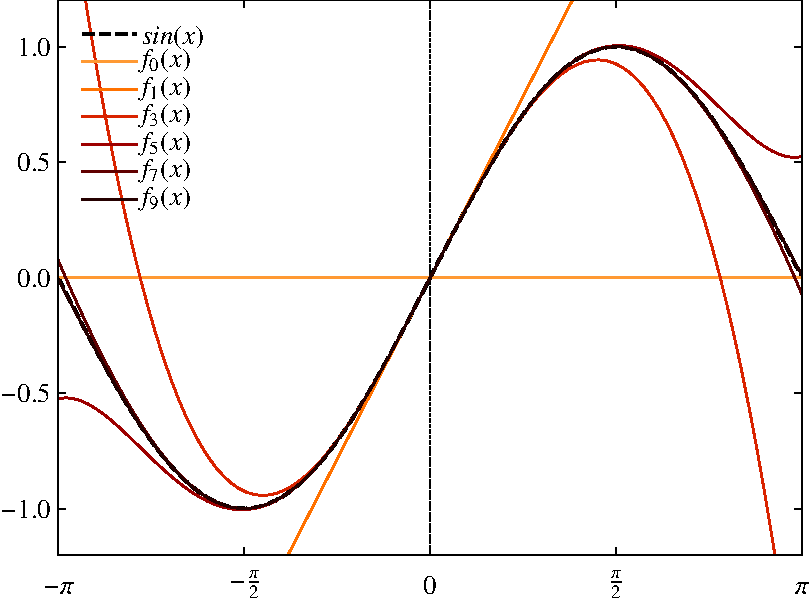
\includegraphics[width=0.6\linewidth]{Pictures/taylor_series_sin}
	\caption{Taylor series expansion of $sin(x)$ about $x=0$}
	\label{fig:taylor_series}
\end{figure}

To understand the behaviour of these truncated expansions, we note that their error arises from truncating the higher-order terms of the expansion. Furthermore, when $\Delta x$ is relatively small, the error is dominated by the first truncated term since the higher-order terms rapidly approximate zero as $\Delta x$ decreases. Hence, if we consider an infinite expansion
\begin{equation}
	f(\Delta x) = \Delta x - \frac{\Delta x^3}{6} + \frac{\Delta x^5}{120} - \frac{\Delta x^7}{5040} + \frac{\Delta x^9}{362880} - \frac{\Delta x^{11}}{39916800} + \hdots,
\end{equation}
we note that the leading term omitted from the $f_1(\Delta x)$ approximation behaves like $\Delta x^3$, the leading error term of the $f_1(\Delta x)$ approximation behaves like $\Delta x^5$, and so on. Hence, as we get closer to the expansion point $x=0$, we expect that the error shrinks, and that the rate at which the error shrinks will be proportional to the exponent of the leading truncated term of the expansion.
\begin{jupyternote}
	Check out the Burgers Jupyter notebook \href{\binderurl}{\underline{here}}. You can also download the files from the Gitlab repository \href{\repourl}{\underline{here}}.
\end{jupyternote}
\chapter{Finite Difference Methods}
\section{The First Derivative}

\begin{figure}[htbp]
	\centering
	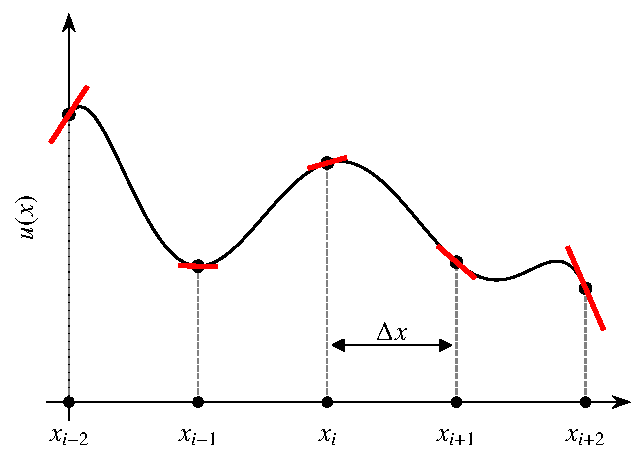
\includegraphics[width=0.6\linewidth]{Pictures/fd_scheme}
	\caption{One-dimensional discretization using Finite Difference methods}
	\label{fig:fd_scheme}
\end{figure}
	
To introduce the finite difference method, we start with a general function $u(x)$. In general, this function can be in any number of dimensions, but for simplicity we will first consider the one-dimensional case. We note that a function can generally be {\it approximated} by its values at a {\it discrete} set of points. An example of this is shown in Figure \ref{fig:fd_scheme} where $\Delta x$ is the grid spacing between the points. We now imagine that we are at some point $i$ whose solution is $u_i = u(x_i)$ where $x_i$ is the physical location of the point. Using Taylor series, we can approximate the value of the solution one grid point to the left from the expansion
\begin{equation}
	u_{i-1} = u_i - \Delta x \Eval{\frac{\partial u}{\partial x}}{x_i}{} + \frac{\Delta x^2}{2} \Eval{\frac{\partial^2 u}{\partial x^2}}{x_i}{} - \frac{\Delta x^3}{6} \Eval{\frac{\partial^3 u}{\partial x^3}}{x_i}{} + \mathcal{O}(\Delta x^4),
	\label{eqn:fdmup}
\end{equation}
where $\mathcal{O}(\Delta x^4)$ denotes the order of the next highest term in the expansion. We can also use another Taylor series to predict the value of the solution one point to the right
\begin{equation}
	u_{i+1} = u_i + \Delta x \Eval{\frac{\partial u}{\partial x}}{x_i}{} + \frac{\Delta x^2}{2} \Eval{\frac{\partial^2 u}{\partial x^2}}{x_i}{} + \frac{\Delta x^3}{6} \Eval{\frac{\partial^3 u}{\partial x^3}}{x_i}{} + \mathcal{O}(\Delta x^4).
	\label{eqn:fdmdwn}
\end{equation}

So far, we have just applied Taylor series to try to determine the solution at points around our initial point $u_i$. However, if we look at Equation \ref{eqn:fdmup} we can use it in a different way. Rearranging we get
\begin{equation}
	\Eval{\frac{\partial u}{\partial x}}{x_i}{} = \frac{u_i - u_{i-1}}{\Delta x} + \frac{\Delta x}{2} \Eval{\frac{\partial^2 u}{\partial x^2}}{x_i}{} - \frac{\Delta x^2}{6} \Eval{\frac{\partial^3 u}{\partial x^3}}{x_i}{} + \mathcal{O}(\Delta x^3).
	\label{eqn:fdmup1}
\end{equation}
We note that as the grid spacing gets smaller, the terms with leading $\Delta x$, $\Delta x^2$, and so on will tend to zero and the approximation
\begin{eqBox}
\begin{equation}
	\Eval{\frac{\partial u}{\partial x}}{x_i}{} = \frac{u_i - u_{i-1}}{\Delta x} + \mathcal{O}(\Delta x),
\end{equation}
\end{eqBox}
will converge to the true value of the derivative at the point $x_i$ as $\Delta x$ tends to zero. We can also do the same trick with Equation \ref{eqn:fdmdwn}. Rearranging, we get
\begin{equation}
	\Eval{\frac{\partial u}{\partial x}}{x_i}{} = \frac{u_{i+1} - u_{i}}{\Delta x} - \frac{\Delta x}{2} \Eval{\frac{\partial^2 u}{\partial x^2}}{x_i}{} - \frac{\Delta x^2}{6} \Eval{\frac{\partial^3 u}{\partial x^3}}{x_i}{} + \mathcal{O}(\Delta x^3),
	\label{eqn:fdmdwn1}
\end{equation}
and again if the grid spacing is small, then the higher-order terms tend to zero and we are left with
\begin{eqBox}
\begin{equation}
	\Eval{\frac{\partial u}{\partial x}}{x_i}{} = \frac{u_{i+1} - u_{i}}{\Delta x} + \mathcal{O}(\Delta x),
\end{equation}
\end{eqBox}
which also allows us to approximate the derivative at $x_i$. Hence, if we know that value of the solution at $x_i$ and either $x_{i-1}$ or $x_{i+1}$ we can approximate the derivative at $x_i$. We note that for both of these approximations, the error in the derivative approximation will decrease proportional to the grid spacing since the leading term in the truncation error is of $\mathcal{O}(\Delta x)$. We refer to a scheme of this form as a {\it first-order} finite difference method.

While the above examples are often useful, they converge rather slowly to the exact value of the derivative at the point $x_i$. However, if we take an average of Equation \ref{eqn:fdmup1} and Equation \ref{eqn:fdmdwn1}, we obtain
\begin{equation}
	\begin{aligned}
	\Eval{\frac{\partial u}{\partial x}}{x_i}{} = &\frac{1}{2}\left(\frac{u_i - u_{i-1}}{\Delta x} + \frac{\Delta x}{2} \Eval{\frac{\partial^2 u}{\partial x^2}}{x_i}{} - \frac{\Delta x^2}{6} \Eval{\frac{\partial^3 u}{\partial x^3}}{x_i}{} \right) + \\
	& \frac{1}{2}\left(\frac{u_{i+1} - u_{i}}{\Delta x} - \frac{\Delta x}{2} \Eval{\frac{\partial^2 u}{\partial x^2}}{x_i}{} - \frac{\Delta x^2}{6} \Eval{\frac{\partial^3 u}{\partial x^3}}{x_i}{} \right) + \mathcal{O}(\Delta x^3)
	\end{aligned}
\end{equation}
which simplifies to
\begin{equation}
	\Eval{\frac{\partial u}{\partial x}}{x_i}{} = \frac{u_{i+1} - u_{i-1}}{2 \Delta x} - \frac{\Delta x^2}{6} \Eval{\frac{\partial^3 u}{\partial x^3}}{x_i}{} + \mathcal{O}(\Delta x^3),
\end{equation}
noting that the leading truncation error terms conveniently cancelled each other out. Hence, if we assume that $\Delta x$ is relatively small, we obtain
\begin{eqBox}
\begin{equation}
	\Eval{\frac{\partial u}{\partial x}}{x_i}{} = \frac{u_{i+1} - u_{i-1}}{2 \Delta x} + \mathcal{O}(\Delta x^2).
\end{equation}
\end{eqBox}
Using this equation, we can approximate the value of the derivative of the function at $x_i$ using the values of the solution at two neighbouring points $x_{i-1}$ and $x_{i+1}$. However, unlike the previous finite difference methods, the truncation error of this approximation is $\mathcal{O}(\Delta x^2)$, meaning that as the grid spacing is reduced, the error will converge like the grid spacing squared. We refer to a scheme of this form as a {\it second-order} finite difference method.

\section{A General Approach}
In the previous section, we derived three different finite difference methods for computing the derivative at a point $x_i$ using the values of the solution at that point and neighbouring points. We have shown that we can create at least two first-order schemes and one second-order scheme. In the current section, we will demonstrate how to generalize this approach to allow us to obtain schemes of any order and for higher-order derivatives.

To start, we will derive a second-order finite difference method to approximate the first derivative using $u_i$, $u_{i-1}$, and $u_{i-2}$. This procedure can be broken down into four basic steps.

\subsection{Step 1: Generate the Taylor Series}
The first step is to expand a Taylor series about each of the points that will be used to approximate the derivative. The Taylor series for $u_{i-1}$ was given before and is
\begin{equation}
	u_{i-1} = u_i - \Delta x \Eval{\frac{\partial u}{\partial x}}{x_i}{} + \frac{\Delta x^2}{2} \Eval{\frac{\partial^2 u}{\partial x^2}}{x_i}{} - \frac{\Delta x^3}{6} \Eval{\frac{\partial^3 u}{\partial x^3}}{x_i}{} + \mathcal{O}(\Delta x^4).
	\label{fdm:general1}
\end{equation}
Similarly, since the distance between $u_i$ and $u_{i-2}$ is $2 \Delta x$ we get the following Taylor series for that point
\begin{equation}
	u_{i-2} = u_i - 2 \Delta x \Eval{\frac{\partial u}{\partial x}}{x_i}{} + \frac{(2\Delta x)^2}{2} \Eval{\frac{\partial^2 u}{\partial x^2}}{x_i}{} - \frac{(2\Delta x)^3}{6} \Eval{\frac{\partial^3 u}{\partial x^3}}{x_i}{} + \mathcal{O}(\Delta x^4).
	\label{fdm:general2}
\end{equation}

\subsection{Step 2: Rearrange the Taylor Series}
The second step is to rearrange each of the Taylor series generated in Step 1 to obtain the derivative of interest on the LHS with everything else on the RHS. Since we are interested in finding an approximation for the first derivative, we rearrange Equation \ref{fdm:general1}
\begin{equation}
	\Eval{\frac{\partial u}{\partial x}}{x_i}{} = \frac{u_i - u_{i-1}}{\Delta x} + \frac{\Delta x}{2}\Eval{\frac{\partial^2 u}{\partial x^2}}{x_i}{} - \frac{\Delta x^2}{6}\Eval{\frac{\partial^3 u}{\partial x^3}}{x_i}{} + \mathcal{O}(\Delta x^3),
	\label{eqn:aHK8G4M7}
\end{equation}
and rearrange Equation \ref{fdm:general1}
\begin{equation}
	\Eval{\frac{\partial u}{\partial x}}{x_i}{} = \frac{u_i - u_{i-2}}{2\Delta x} + \frac{2\Delta x}{2}\Eval{\frac{\partial^2 u}{\partial x^2}}{x_i}{} - \frac{(2\Delta x)^2}{6}\Eval{\frac{\partial^3 u}{\partial x^3}}{x_i}{} + \mathcal{O}(\Delta x^3),
	\label{eqn:6sbrhgAM}
\end{equation}
which gives two expressions for the first derivative.

\subsection{Step 3: Determine a Suitable Combination}
If we look at the previous two expressions for the first derivative, we will notice that they are both first-order accurate since the leading term that will get truncated is $\mathcal{O}(\Delta x)$. However, we were tasked with finding a second-order accurate scheme. In order to achieve this, we will try to combine Equation \ref{eqn:aHK8G4M7} and Equation \ref{eqn:6sbrhgAM} in such a way the first-order error term cancels out.

We want to combine them is such a way that
\begin{equation}
	\Eval{\frac{\partial u}{\partial x}}{x_i}{} = a(\ref{eqn:aHK8G4M7}) + b(\ref{eqn:6sbrhgAM}),
	\label{eqn:2KGWrZa5}
\end{equation}
gives a second-order approximating for the first derivative, and we need to find the coefficients $a$ and $b$ to achieve this. If we look at the left-hand side, we want to keep the first derivative there. This can be achieved if we ensure that
\begin{equation}
	a + b = 1.
	\label{eqn:3Wxy2aCD}
\end{equation}
The second thing we need to do is cancel out the $\mathcal{O}(\Delta x)$ term to ensure that the leading truncation error term is $\mathcal{O}(\Delta x^2)$. Looking at the $\mathcal{O}(\Delta x)$ terms, in order for them to cancel out, we require
\begin{equation}
	\frac{a}{2} + b = 0.
	\label{eqn:rWD4Hs8v}
\end{equation}
Equations \ref{eqn:3Wxy2aCD} and \ref{eqn:rWD4Hs8v} are recognizable as a linear system of equations with two equations and two unknowns. This can be readily solved using substitution yielding $a=2$ and $b=-1$.

\subsection{Step 3: Combine the Schemes}
Now that we have determined the constants in Equation \ref{eqn:2KGWrZa5}, the last step is to just go ahead and add things together. Doing this will yield that following finite difference approximation
\begin{eqBox}
\begin{equation}
	\Eval{\frac{\partial u}{\partial x}}{x_i}{} = \frac{3u_i - 4u_{i-1} + u_{i-2}}{2 \Delta x} + \mathcal{O}(\Delta x^2),
	\label{eqn:aHK8G4M7}
\end{equation}
\end{eqBox}
which is a second-order approximation of the first derivative use three points. Hence, we have accomplished our task.

\section{The Second Derivative}
In the previous sections, we derived four different schemes for the first derivative, two that were first-order accurate, and two that were second-order accurate. However, if we go back and look at the Navier-Stokes equations, we will note that we also need to approximate second-derivatives for the diffusive terms. We will derive an example scheme here, which also demonstrates another application of the four basic steps of creating a finite difference scheme. Our objective will be to derive a second-order finite difference method to approximate the second derivative using $u_i$, $u_{i-1}$, and $u_{i+1}$.

We now recall that the first step was to simply expand a Taylor series about all of the points that are not $u_i$. We have already derived these expansions for $u_{i-1}$ and $u_{i+1}$, which are
\begin{equation}
	u_{i-1} = u_i - \Delta x \Eval{\frac{\partial u}{\partial x}}{x_i}{} + \frac{\Delta x^2}{2} \Eval{\frac{\partial^2 u}{\partial x^2}}{x_i}{} - \frac{\Delta x^3}{6} \Eval{\frac{\partial^3 u}{\partial x^3}}{x_i}{} + \mathcal{O}(\Delta x^4),
	\label{eqn:Bm6Tq8Ah}
\end{equation}
and
\begin{equation}
	u_{i+1} = u_i + \Delta x \Eval{\frac{\partial u}{\partial x}}{x_i}{} + \frac{\Delta x^2}{2} \Eval{\frac{\partial^2 u}{\partial x^2}}{x_i}{} + \frac{\Delta x^3}{6} \Eval{\frac{\partial^3 u}{\partial x^3}}{x_i}{} + \mathcal{O}(\Delta x^4).
	\label{eqn:93Nxbhtu}
\end{equation}
So that is step one done.

In step two, we needed to rearrange these equations such that the derivative of interest is on the LHS. This yields two possible expressions for the second derivative by rearranging Equation \ref{eqn:Bm6Tq8Ah}
\begin{equation}
	\Eval{\frac{\partial^2 u}{\partial x^2}}{x_i}{} = \frac{2(u_{i-1} - u_i)}{\Delta x^2} + \frac{2}{\Delta x} \Eval{\frac{\partial u}{\partial x}}{x_i}{} + \frac{\Delta x}{3} \Eval{\frac{\partial^3 u}{\partial x^3}}{x_i}{} + \mathcal{O}(\Delta x^2),
\end{equation}
and Equation \ref{eqn:93Nxbhtu}
\begin{equation}
	\Eval{\frac{\partial^2 u}{\partial x^2}}{x_i}{} = \frac{2(u_{i+1} - u_i)}{\Delta x^2} - \frac{2}{\Delta x} \Eval{\frac{\partial u}{\partial x}}{x_i}{} - \frac{\Delta x}{3} \Eval{\frac{\partial^3 u}{\partial x^3}}{x_i}{} + \mathcal{O}(\Delta x^2),
\end{equation}
noting that the $\mathcal{O}(\Delta x^4)$ terms are now $\mathcal{O}(\Delta x^2)$ since we had to divide the RHS by $\Delta x^2$. That marks the end of step two.

In the third step, we have to determine a linear combination of these two equations that will give us an expression for the second derivative with a truncation error of $\mathcal{O}(\Delta x^2)$. Since we want to keep the second derivative on the LHS, we require
\begin{equation}
	a + b = 1.
\end{equation}
And, in order for the truncation error to be of $\mathcal{O}(\Delta x^2)$, we need to cancel the second and third terms on the RHS of the equations, which are $\mathcal{O}(\Delta x^{-1})$ and $\mathcal{O}(\Delta x)$, respectively. Interestingly, cancelling out both of these terms requires
\begin{equation}
	a - b = 0.
\end{equation}
Once again, we have a linear system with two equations and two unknowns. Solving this system yields $a=b=1/2$, which finishes part three.

Finally, in part four, we simply combine the two equations multiplied by their respective $a$ and $b$ coefficients. This yields our second-order accurate expression for the second-derivative as
\begin{eqBox}
\begin{equation}
	\Eval{\frac{\partial^2 u}{\partial x^2}}{x_i}{} = \frac{u_{i-1} - 2u_i + u_{i+1}}{\Delta x^2} + \mathcal{O}(\Delta x^2).
\end{equation}
\end{eqBox}

\section{Example Applications}
Now that we have created a few introductory finite difference methods, it is time to put them to work on our three simplified systems.
\subsection{Linear Advection}
We recall that the one-dimensional linear advection equation in differential form was
\begin{equation}
	\frac{\partial u}{\partial t} +  \alpha \frac{\partial u}{\partial x} = 0.
\end{equation}
In the previous sections, we derived a few options for this, but to start we will use the simple first-order upwind scheme to approximate the spatial derivative at each grid point, such that
\begin{equation}
	\Eval{\frac{\partial u}{\partial x}}{x_i}{} = \frac{u_i^t - u_{i-1}^t}{\Delta x} + \mathcal{O}(\Delta x),
\end{equation}
where the superscript $t$ denotes that we are using the solution at the current time. We will also use a first-order finite difference approach in time to approximate the temporal derivative as well. Hence,
\begin{equation}
	\Eval{\frac{\partial u}{\partial t}}{x_i}{} = \frac{u_i^{t+1} - u_{i}^t}{\Delta t} + \mathcal{O}(\Delta t),
\end{equation}
where $\Delta t$ is the time step size and the superscript $t+1$ is the solution at the next time step.

Now we simply insert these approximations into the linear advection equation, yielding
\begin{equation}
	\frac{u_i^{t+1} - u_{i}^t}{\Delta t} +  \alpha \frac{u_i^t - u_{i-1}^t}{\Delta x} + \mathcal{O}(\Delta x, \Delta t) = 0.
\end{equation}
By inspecting this equation, and assuming that we know the solution at each grid point at the current instant in time, we can rearrange this to make a prediction for the solution at the next time step
\begin{eqBox}
\begin{equation}
	u_i^{t+1} = u_{i}^t -\frac{\alpha \Delta t}{\Delta x} \left( u_i^t - u_{i-1}^t \right) + \mathcal{O}(\Delta x, \Delta t).
	\label{eqn:7hH8UBeG}
\end{equation}
\end{eqBox}

Looking at Equation \ref{eqn:7hH8UBeG}, we note that, provided we know the current solution at all grid points at time $t$, we can predict the solution at time $t+\Delta t$ with an error term of $\mathcal{O}(\Delta x, \Delta t)$. Then we will have an approximation of the solution at all grid points at time $t+\Delta t$, and we can use this to find an approximation of the solution at time $t+2\Delta t$ by applying the same equation, and so on. Hence, we are able to advance the linear advection equation to any final time we desire, noting that each time step we take will introduce some numerical error. A series of example solutions using different numbers of grid points is shown in Figure \ref{fig:advection_upwind} with an advection velocity of $\alpha = 1$, and a final solution time of $t=1$, which allows the Gaussian bump to travel once through the domain. If the error is measured in terms of the height of the peak of the Gaussian bump, it is apparent that it converges linearly as the grid spacing is refined.
\begin{figure}[htbp]
	\centering
	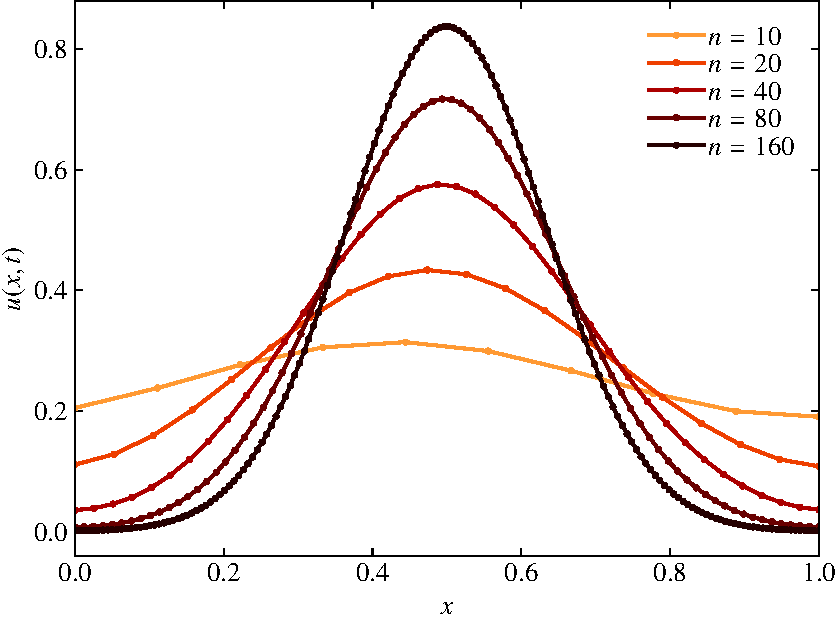
\includegraphics[width=0.65\linewidth]{Pictures/advection_upwind}
	\caption{First-order advection of a gaussian bump using different levels of grid refinement.}
	\label{fig:advection_upwind}
\end{figure}
\begin{jupyternote}
	Check out the Advection Jupyter notebook \href{\binderurl}{\underline{here}}. You can also download the files from the Gitlab repository \href{\repourl}{\underline{here}}.
\end{jupyternote}
\subsection{Burgers Equation}
We recall that the one-dimensional Burgers equation was
\begin{equation}
	\frac{\partial u}{\partial t} +  \frac{1}{2} \frac{\partial u^2}{\partial x} = 0.
\end{equation}
We can now use the exact same approach for Burgers as we used for the linear advection equation. First, we will use a first-order upwind approach to approximate the spatial derivative of $u^2$ at each grid point $x_i$, such that
\begin{equation}
	\Eval{\frac{\partial u^2}{\partial x}}{x_i}{} = \frac{(u_i^t)^2 - (u_{i-1}^t)^2}{\Delta x} + \mathcal{O}(\Delta x),
\end{equation}
where again the superscript $t$ denotes that we are using the solution at the current time. We will also use a first-order finite difference approach in time to approximate the temporal derivative as well. Hence,
\begin{equation}
	\Eval{\frac{\partial u}{\partial t}}{x_i}{} = \frac{u_i^{t+1} - u_{i}^t}{\Delta t} + \mathcal{O}(\Delta t).
\end{equation}

Now, we simply insert our finite difference approximations of these two derivatives into the Burgers equation
\begin{equation}
	\frac{u_i^{t+1} - u_{i}^t}{\Delta t} +  \frac{1}{2}\frac{(u_i^t)^2 - (u_{i-1}^t)^2}{\Delta x} + \mathcal{O}(\Delta x, \Delta t) = 0,
\end{equation}
and, just like for linear advection, we can now find an expression for the solution at any grid point at the next time step as
\begin{eqBox}
\begin{equation}
	u_i^{t+1} = u_{i}^t - \frac{\Delta t}{\Delta x} \frac{1}{2}\left( \left(u_i^t \right)^2 - \left( u_{i-1}^t \right)^2 \right) + \mathcal{O}(\Delta x, \Delta t).
	\label{eq:fd_burgers}
\end{equation}
\end{eqBox}
Looking at this expression, we note it is remarkably similar to the expression for linear advection, which is not particularly surprising as the two initial partial differential equations are also quite similar. Again, if we know the solution at each grid point at some time $t$, we can approximate the solution at some time $t+\Delta t$ using this expression. Then, to approximate the solution at the time $t+2\Delta t$ we simply re-apply the expression. This allows us to approximate the behaviour of Burgers equation up to any desired final time, and the error of the approximation is expected to be first-order accurate in both space and time, with errors on the order of $\mathcal{O}(\Delta x, \Delta t)$. A series of example solutions using different numbers of grid points is shown in Figure \ref{fig:burgers_upwind}.

\begin{figure}[htbp]
	\centering
	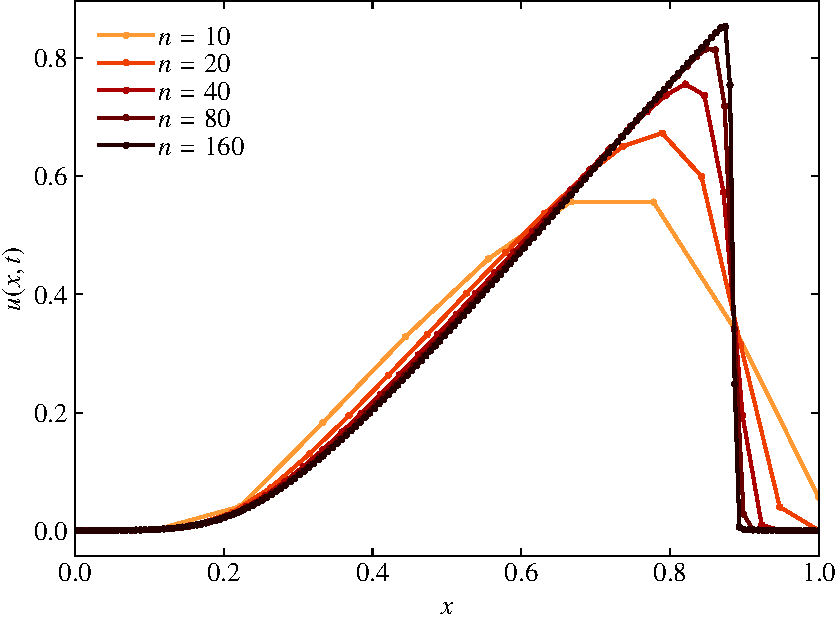
\includegraphics[width=0.65\linewidth]{Pictures/burgers_upwind}
	\caption{First-order nonlinear burgers equation with a gaussian bump using different levels of grid refinement.}
	\label{fig:burgers_upwind}
\end{figure}
\begin{jupyternote}
	Check out the Burgers Jupyter notebook \href{\binderurl}{\underline{here}}. You can also download the files from the Gitlab repository \href{\repourl}{\underline{here}}.
\end{jupyternote}

\subsection{Linear Diffusion}
We recall that our third and final simplified system of equations was the linear diffusion equation
\begin{equation}
\frac{\partial u}{\partial t} - \beta \frac{\partial^2 u}{\partial x^2} = 0,
\end{equation}
which described how some conserved quantity, such as heat, diffuses into the surrounding fluid. To approximate this using the finite difference method, we follow the exact same steps as for linear advection and Burgers equation. First, we will use our second-order accurate finite difference approximation for the second derivative as
\begin{equation}
	\Eval{\frac{\partial^2 u}{\partial x^2}}{x_i}{} = \frac{u_{i-1} - 2u_i + u_{i+1}}{\Delta x^2} + \mathcal{O}(\Delta x^2).
\end{equation}
We will also use a first-order finite difference approach in time to approximate the temporal derivative as well. Hence,
\begin{equation}
	\Eval{\frac{\partial u}{\partial t}}{x_i}{} = \frac{u_i^{t+1} - u_{i}^t}{\Delta t} + \mathcal{O}(\Delta t).
\end{equation}

Now we simply replace the exact derivatives in the linear diffusion equation with our finite difference approximations, such that
\begin{equation}
\frac{u_i^{t+1} - u_{i}^t}{\Delta t} - \beta \frac{u_{i-1} - 2u_i + u_{i+1}}{\Delta x^2} + \mathcal{O}(\Delta x^2,\Delta t) = 0.
\end{equation}
Again, by simply rearranging we can arrive at an expression for the solution at any grid point $i$ at the next time step as
\begin{eqBox}
\begin{equation}
u_i^{t+1}  = u_{i}^t + \frac{\beta \Delta t}{\Delta x^2} \left(u_{i-1} - 2u_i + u_{i+1}\right) + \mathcal{O}(\Delta x^2,\Delta t).
\label{eq:fd_diffusion}
\end{equation}
\end{eqBox}
Again, this is very similar to the approximations for linear advection and Burgers equations. However, one important thing to note is that the error in space is of $\mathcal{O}(\Delta x^2)$ instead of $\mathcal{O}(\Delta x)$, meaning that as we refine the grid the solution will converge more quickly to the exact solution of the linear diffusion equation.
\begin{figure}[htbp]
	\centering
	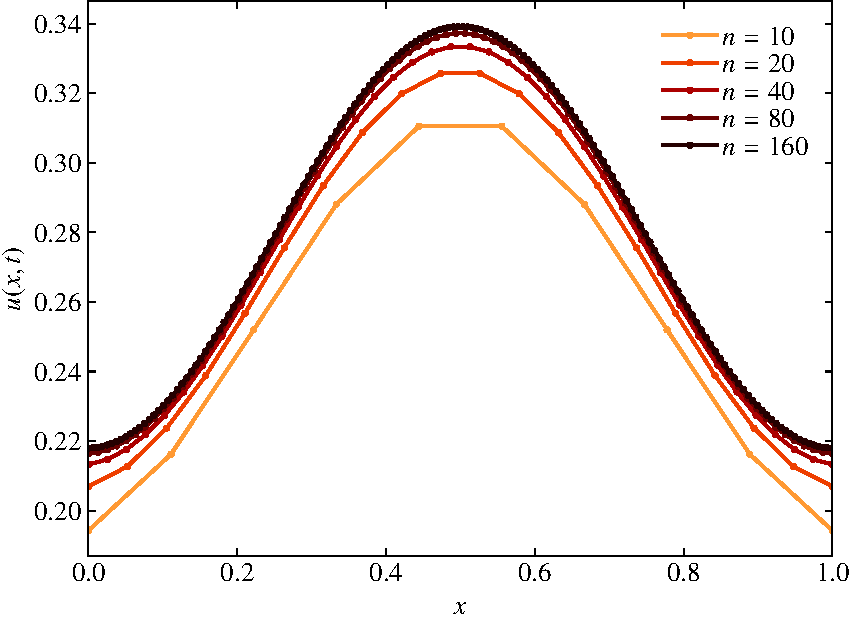
\includegraphics[width=0.65\linewidth]{Pictures/diffusion_central}
	\caption{Second-order linear diffusion of a gaussian bump using different levels of grid refinement and $\alpha=1\times 10^{-3}$.}
	\label{fig:diffusion_central}
\end{figure}
\begin{jupyternote}
	Check out the Diffusion Jupyter notebook \href{\binderurl}{\underline{here}}. You can also download the files from the Gitlab repository \href{\repourl}{\underline{here}}.
\end{jupyternote}

\chapter{Finite Volume Methods}
\begin{figure}[htbp]
 \centering
 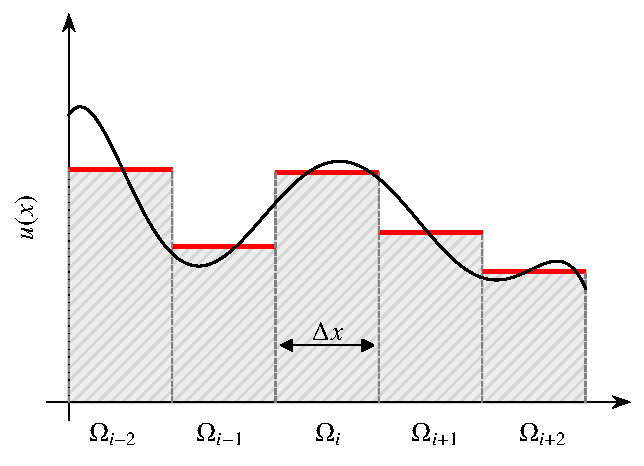
\includegraphics[width=0.6\linewidth]{Pictures/fv_scheme}
 \caption{One-dimensional Finite Volume discretization}
 \label{fig:fv_scheme}
\end{figure}
In the previous chapter, we derived and characterized the finite difference method. While it is generally simple to apply, it requires the use of structured grids. Suppose now you want to simulate flow over an aircraft or one of its components. Generating structured meshes can become challenging, if not impossible, for complex geometries. Hence, we need methods that are flexible enough such that the geometry is not a fundamental limitation. Instead of evaluating the solution in a pointwise fashion, consider subdividing a generic domain $\Omega$ into volumes or cells $\Omega_i$, as shown in Figure~\ref{fig:fv_scheme}. Within each cell, the value of the function $u(x)$ can be assumed constant and is calculated using an integral approach. This idea leads to the derivation of the finite volume method, which is one of the most commonly used spatial discretizations in industry. It was initially developed for its application on the general form of the conservation laws, meaning it can be fundamentally applied to solutions that present discontinuities. In this chapter, we present the theory required to apply the finite volume method on scalar as well as systems of conservation laws. Additional useful references include~\cite{levequeFiniteVolumeMethods2002,hirschNumericalComputationInternal2007a,andersonComputationalFluidMechanics2016, toroRiemannSolversEvolved2006}.

\section{Derivation}
Consider the general conservation law applied to a volume of arbitrary shape $\Omega$, as shown in Figure~\ref{fig:fv_omega}
\begin{figure}[htbp]
 \centering
 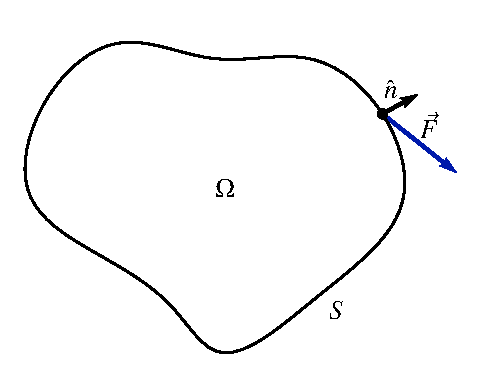
\includegraphics[width=0.4\linewidth]{Pictures/fv_arbitrary_volume}
 \caption{Representation of an arbitrary volume of undefined shape.}
 \label{fig:fv_omega}
\end{figure}
\begin{equation}
 \int_\Omega \frac{\partial \vec u}{\partial t} d \Omega + \int_s \vec F\cdot \hat n ds = 0,
 \label{eq:fv_gcl}
\end{equation}
where $\vec{u}$ is a vector of conserved variables, such as mass, momentum, and energy. $\vec{F}=\vec F(\vec u)$ is the vector of fluxes, $S$ is the area of $\Omega$ with outward unit normal $\hat n$. Recall that for constant volumes, integration and differentiation commute so we can rewrite Equation~\ref{eq:fv_gcl}
\begin{equation}
 \frac{d}{dt} \int_\Omega \vec{u} d\Omega + \int_s \vec F\cdot \hat n ds = 0.
 \label{eq:fv_gclleibniz}
\end{equation}
Clearly, the integral of the solution represents its total amount within $\Omega$. Hence, the rate of change of the total amount of $\vec{u}$ in a volume is the result of the net flux across the surface $S$ of $\Omega$. As we have stated in the introduction of this chapter, we are looking for averaged values of the solution, specifically the \textit{cell-average} of $\vec u$, which is given by
\begin{equation}
 \vec {\overline{u}} = \frac{ \int_\Omega \vec u d\Omega} {|\Omega|},
 \label{eq:fv_average}
\end{equation}
where $|\Omega|$ is the size of the cell. After averaging the solution, it is clear that it has become constant within each volume, i.e. $\vec {\overline u} \neq \vec {\overline u} (\vec x)$, so it is now only a function of time $\overline {\vec u} = \overline {\vec u} (t)$. If we combine Equations~\ref{eq:fv_gclleibniz} and~\ref{eq:fv_average}, we obtain
\begin{equation}
 \frac{d \vec{\overline u}}{dt} + \frac{1}{|\Omega|} \int_s \vec{F} \cdot\hat nds=0.
\end{equation}
Now, we have an equation for the rate of change of the averaged quantity $\vec{\overline u}$. What remains is to define the value of $\vec{F}$. First, we note that the averaged solution $\vec{\overline u}$ must converge to the instantaneous solution $\vec{u}$ in the limit of sufficiently small volumes
\begin{align}
 \lim_{|\Omega| \rightarrow 0} \vec{\overline u} = \vec u,
\end{align}
and hence,
\begin{equation}
 \lim_{|\Omega| \rightarrow 0} \vec F (\vec {\overline{u}}) = \vec F(\vec u).
\end{equation}
This leads to the general form of the finite volume method, which we write 
\begin{eqBox}
\begin{equation}
 \frac{d \vec{\overline u}}{dt} = - \frac{1}{|\Omega|} \int_s \vec{F} (\vec{\overline u})\cdot\hat nds=0,
 \label{eq:fvm}
\end{equation}
\end{eqBox}
where $d/dt$ can be solved using an appropriate temporal discretization (see Chapter~\ref{ch:timestepping}). 

Generally, we can make relatively good approximations of arbitrary volumes using straight-sided elements such as triangles and tetrahedra. Consider the triangular volume $\Omega_i$ displayed in Figure~\ref{fig:fv_straightsided}. The solution $\vec{\overline u}$ is constant within the triangular shape. In addition, each of the faces has an area of $S_1$, $S_2$ and $S_3$. Observe that since the sides of the considered volume are straight, the flux vectors are constant across each of the faces. Hence, the surface integral in Equation~\ref{eq:fvm} can be trivially solved via summation. For the $i$-th volume, the general form of the FV method for straight grids can be written
\begin{figure}[htbp]
 \centering
 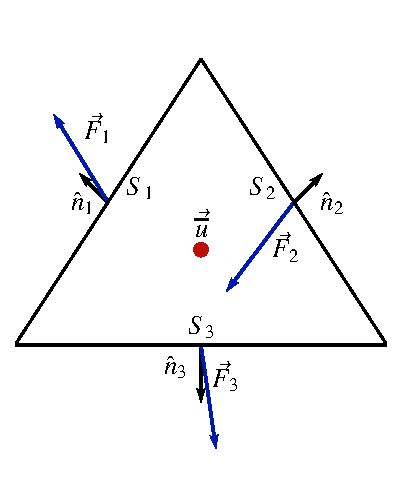
\includegraphics[width=0.3\linewidth]{Pictures/fv_cellavg}
 \caption{Representation of solution, fluxes and faces of a straight-sided element.}
 \label{fig:fv_straightsided}
\end{figure}
\begin{eqBox}
 \begin{equation}
 \frac{d \overline{\vec u}_i}{dt} = - \frac{1}{|\Omega_i|} \sum_{j=1}^{m} \vec F_j \cdot \hat n_j S_j,
 \label{eq:fv_straightsided}
 \end{equation}
\end{eqBox}
where $m$ is the number of faces, $F_i$ is the flux across the $j$-th face with outward unit normal $\hat n_j$ and area surface $S_j$.

\section{The Riemann Problem}
\begin{figure}[htbp]
 \centering
 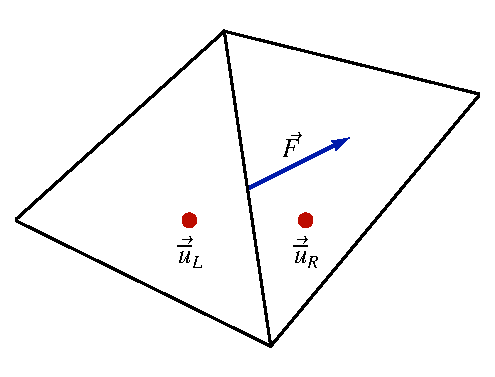
\includegraphics[width=0.4\linewidth]{Pictures/fv_riemann_diagram}
 \caption{Representation of the Riemann problem}
 \label{fig:fv_riemannproblem}
\end{figure}
You may now realize that the solution is piecewise linear, i.e., we have approximated a function $\vec u(x,t)$ by constant values $\vec {\overline u}_i(t)$ at each volume $\Omega_i$. Usually, in finite difference methods, the value of the flux can be simply computed as $\vec{F}=\vec{F}(\vec{\overline{u}})$ due to the pointwise approach. In contrast, consider the two volumes shown in Figure~\ref{fig:fv_riemannproblem} as a result of a finite volume discretization. We are looking for the value of the fluxes across each of the volume's faces to solve Equation~\ref{eq:fv_straightsided}. However, note that on each side of the interface, we have two values of the solution $\vec{\overline{u}}_L,~\vec{\overline{u}}_R$, which are expected to yield a single value of the flux. Hence, the flux at the interface is
\begin{eqBox}
 \begin{equation}
 \vec{F} = \vec{F} (\vec{\overline{u}}_L,~\vec{\overline{u}}_R).
 \end{equation}
\end{eqBox}
This is known as the \textit{Riemann problem}. The solution to the Riemann problem depends on the physics of the problem. For hyperbolic equations, it is said to be a similarity solution and is related to the \textit{characteristic speed} of the PDE. We now present some examples of the Riemann problem for scalar conservation laws and the resulting finite-volume discretizations. Later in this chapter, we will come back to this topic and derive some solutions for systems of hyperbolic equations.

\section{Example Applications}
We have now derived the finite volume method and described some of its characteristics. We have introduced a consequence of the discretization, which is the Riemann problem. In this section, we present finite-volume schemes applied to our simple one-dimensional scalar conservation laws, as well as solutions to the Riemann problem for each of these equations.
\subsection{Linear Advection}
Consider the general conservation law applied to the one-dimensional advection equation. For scalar conservation laws, we may write
\begin{equation}
 \vec{u} = u,
\end{equation}
and hence the advection flux is given by
\begin{equation}
 \vec{F} = f = \alpha u,
\end{equation}
where $\alpha$ is the advection velocity. A finite-volume discretization for this problem can be seen in Figure~\ref{fig:fv_advection}, where $\alpha >0$. Consider the cell $\Omega_i$. We need to find the value of the flux at each of the faces of the cell. 
\begin{figure}[htbp]
 \centering
 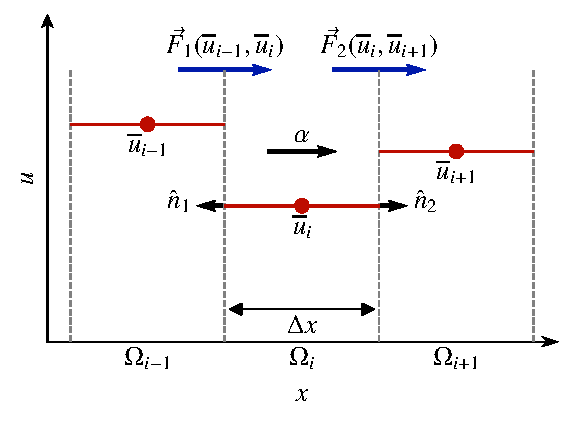
\includegraphics[width=0.5\linewidth]{Pictures/fv_advection}
 \caption{Finite-volume linear advection.}
 \label{fig:fv_advection}
\end{figure}
Different approaches can be considered, which result in distinct finite-volume schemes, each with its own characteristic error and order of accuracy. We now present three options to compute the Riemann flux and the resulting discretizations.
\subsubsection{Upwind}
We have previously assumed $\alpha>0$, which means information travels from left to right. A natural choice of Riemann flux is \textit{upwind}. Here, the value of the flux is computed from the left-hand-side solution value at each interface. Hence, 
\begin{equation}
 \vec F(\overline u_L, \overline u_R) = \alpha \overline u_L, 
\end{equation}
which can be written 
\begin{align}
 \vec F_1 &= \alpha \overline u_{i-1}, \\ 
 \vec F_2 &= \alpha \overline u_{i},
\end{align}
for the left and right faces of $\Omega_i$, respectively. Recall the finite-volume discretization for straight-sided elements in Equation~\ref{eq:fv_straightsided}, which we now rewrite for this problem considering $\hat n_1=-1$, $\hat n_2=1$ and $S_1=S_2=1$
\begin{equation}
 \frac{d \overline{u}_i}{dt} = -\frac{1}{\Delta x} \left(\alpha \overline {u}_i - \alpha \overline u_{i-1}\right),
\end{equation}
or simply
\begin{eqBox}
\begin{equation}
 \frac{d \overline{u}_i}{dt} = -\alpha \frac{ \overline {u}_i - \overline u_{i-1}}{\Delta x},
\end{equation}
\end{eqBox}
which is identical to the original first-order finite-difference method. Discretizing the temporal derivative using the forward Euler method, we have
\begin{eqBox}
\begin{equation}
\overline u_i^{t+1} = \overline u_i^t - \frac{\alpha \Delta t}{\Delta x} \left( \overline {u}_i^t - \overline u_{i-1}^t\right).
\end{equation}
\end{eqBox}
Hence, by comparing the above equation with Equation~\ref{eqn:7hH8UBeG}, we can see that they are indentical.
\subsubsection{Central}
A second choice of Riemann flux results from an averaged value of the solution at each interface. This means
\begin{equation}
 \vec F(\overline u_L, \overline u_R) = \frac{1}{2}\left(\alpha \overline u_L + \alpha \overline u_R \right).
\end{equation}
Hence, the fluxes can be written
\begin{align}
 \vec F_1 = \frac{1}{2}\left(\alpha \overline u_{i-1} + \alpha \overline u_{i} \right),\\
 \vec F_2 = \frac{1}{2}\left(\alpha \overline u_{i} + \alpha \overline u_{i+1} \right),
\end{align}
for the left and right interface of $\Omega_i$, respectively. By substituting these fluxes into Equation~\ref{eq:fv_straightsided}, a central finite-volume scheme can be written
\begin{eqBox}
\begin{equation}
 \frac{d\overline u_i}{dt} = - \alpha \frac{\overline u_{i+1} - u_{i-1}}{2 \Delta x},
\end{equation}
\end{eqBox}
which is identical to the second-order finite-difference method. 
\subsubsection{Blended}
Consider upwind and central fluxes given by
\begin{align}
 f_u & = \alpha \overline u_L, \\
 f_c & = \frac{\alpha}{2} \left(\overline u_L + \overline u_R \right),
\end{align}
respectively, where $f_u$ yields a \textit{low-resolution} first order scheme and $f_c$ yields a second-order, \textit{high-resolution} scheme. We can combine these two approaches to obtain a \textit{blended} scheme, such that
\begin{eqBox}
\begin{equation}
 f_b = f_u + \phi f_c,
\end{equation}
\end{eqBox}
where $\phi$ is a weighting parameter that can recover the upwind, central or yield a blended scheme, i.e.
\[
 f = 
\begin{cases}
 f_u & \text{if}~\phi = 0, \\
 f_c & \text{if}~\phi = 1, \\ 
 f_b & \text{if}~0 < \phi < 1. 
\end{cases}
\]
We have shown that we can recover finite-difference schemes on structured grids for the linear advection equation considering appropriate choices for the Riemann solver. We now explore whether this is also true for the Burgers equation.
\subsection{Burgers Equation}
We now consider the Burgers equation. As we have previously stated, for scalar conservation laws
\begin{equation}
 \vec{u} = u,
\end{equation}
and in the case of Burgers, the flux can be written
\begin{equation}
 \vec{F} = f(u) = \frac{1}{2} u^2.
\end{equation}
Recall that solutions in Burgers equation tend to develop discontinuities at a finite time even if they are initially smooth. Hence, a common Riemann flux choice for this problem is upwind due to its dissipative effect. We can write the fluxes at each face of $\Omega_i$
\begin{align}
 F_1 &= \frac{1}{2} \overline u_{i-1}^2, \\ 
 F_2 &= \frac{1}{2} \overline u_{i}^2.
\end{align}
By following the same procedure as with the advection equation, we obtain the semidiscrete scheme from Equation~\ref{eq:fv_straightsided}, 
\begin{equation}
 \frac{d\overline u_i}{dt} = - \frac{1}{\Delta x} \left(\frac{\overline u_i^2}{2} - \frac{\overline u_{i-1}^2}{2}\right),
\end{equation}
which we simplify
\begin{eqBox}
\begin{equation}
 \frac{d\overline u_i}{dt} = - \frac{1}{2 \Delta x} \left(\left(\overline u_i\right)^2 - \left(\overline u_{i-1}\right)^2\right).
 \label{eq:fv_burgers}
\end{equation}
\end{eqBox}
Applying the first-order forward Euler scheme to advance the solution in time yields
\begin{eqBox}
	\begin{equation}
	 \overline u_i^{t+1} = \overline u_i^t - \frac{\Delta t}{\Delta x} \frac{1}{2} \left(\left(\overline u_i^t\right)^2 - \left(\overline u_{i-1}^t \right)^2\right).
	 \label{eq:fv_burgers_fully}
	\end{equation}
\end{eqBox}
Equation~\ref{eq:fv_burgers_fully} is identical to the first-order upwind scheme for Burgers equation derived using finite difference in Equation~\ref{eq:fd_burgers}.
\subsection{Linear Diffusion}
Consider the scalar linear diffusion equation, where
\begin{equation}
 \vec{u} = u,
\end{equation}
and the corresponding flux can be obtained from Fourier's law
\begin{equation}
 \vec{F} = f = -\beta \frac{\partial u}{\partial x},
\end{equation}
where $\beta$ is a constant diffusion coefficient. The resulting finite-volume discretization for this problem can be observed in Figure~\ref{fig:fv_diffusion}. Note that at each interface, we need to compute the derivative of the solution. Due to the behaviour of the diffusion equation, one should expect the Riemann flux to include the effects from both sides of the element.
\begin{figure}[htbp]
 \centering
 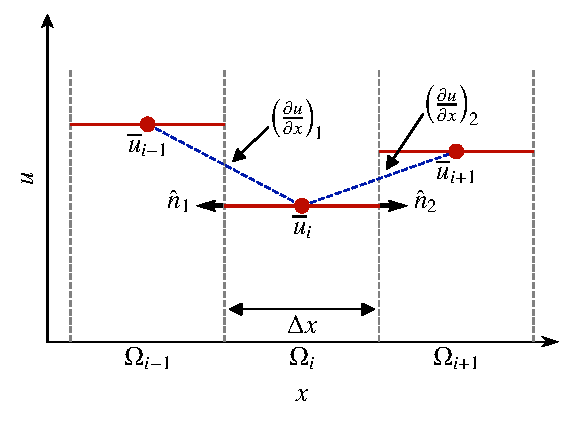
\includegraphics[width=0.5\linewidth]{Pictures/fv_diffusion}
 \caption{Finite-volume linear diffusion.}
 \label{fig:fv_diffusion}
\end{figure}
We can compute the derivatives considering an upwind and a downwind difference approach at the left and right faces , respectively. Hence,
\begin{align}
 \left(\frac{\partial u}{\partial x}\right)_1 & \approx \frac{\overline u_i - \overline u_{i-1}}{\Delta x}, \\
 \left(\frac{\partial u}{\partial x}\right)_2 & \approx \frac{\overline u_{i+1} - \overline u_{i}}{\Delta x}.
\end{align}
Then the respective fluxes can be computed from
\begin{align}
 \vec F_1 &=-\beta \left(\frac{\partial u}{\partial x}\right)_1 \approx -\beta \frac{\overline u_i - \overline u_{i-1}}{\Delta x},\\
 \vec F_2 &=-\beta \left(\frac{\partial u}{\partial x}\right)_2 \approx -\beta \frac{\overline u_{i+1} - \overline u_{i}}{\Delta x}.
\end{align}
By substituting the fluxes into Equation~\ref{eq:fv_straightsided}, we obtain the finite-volume method for linear diffusion
\begin{eqBox}
 \begin{equation}
 \frac{d\overline u_i}{dt} = \beta \frac{\overline u_{i+1}-2\overline u_{i} + \overline u_{i-1}}{\Delta x^2},
	\label{eq:fv_diffusion}
 \end{equation}
\end{eqBox}
which is second-order accurate. The resulting scheme is central, which agrees with the physics of diffusive processes.  If we couple the spatial derivative in Equation~\ref{eq:fv_diffusion} with the forward Euler method, we can write the fully-discrete scheme
\begin{eqBox}
\begin{equation}
	\overline u_i^{t+1} = \overline u_i^t + \frac{\beta \Delta t}{\Delta x^2}  \left(\overline u_{i+1}^t-2\overline u_{i}^t + \overline u_{i-1}^t\right).
	\label{eq:fv_diffusion_fullydiscrete}
\end{equation}
\end{eqBox}
Note that Equation~\ref{eq:fv_diffusion} is identical to the second-order finite-difference scheme we previously derived for this problem in Equation~\ref{eq:fd_diffusion}.  
\section{Linear Hyperbolic Problems} \label{sec:linear_hyperb_problems}
In Chapter 2, we stated that first-order partial differential equations are naturally hyperbolic, meaning that they exhibit wave-like solutions. The simplest case is our advection equation
\begin{equation}
	\frac{\partial u}{\partial t} + \alpha \frac{\partial u}{\partial x} = 0, 
	\label{eq:hyperprob_advection}
\end{equation}
\begin{figure}[htbp]
	\centering
	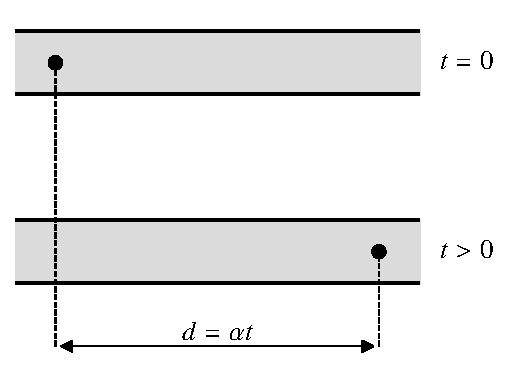
\includegraphics[width=0.5\linewidth]{Pictures/lsc_advection_dye}
	\caption{Initial and final state of the advection of a dye particle in a one-dimensional flow.}
	\label{fig:advection_dye}
\end{figure}
which can model, for instance, the tracing of a dye particle in a one-dimensional geometry, such as a pipe. Suppose that you want to trace this particle. At time $t=0$, the particle is located at $x=0$ as shown in Figure~\ref{fig:advection_dye}. After some time, we expect the particle to have translated a distance $d=\alpha t$. Hence, it can be easily checked that solutions to Equation~\ref{eq:hyperprob_advection} are given by
\begin{equation}
	u(x,t) = u_0 (x - \alpha t), 
\end{equation}
where $u_0$ is the initial solution. Note that the particle has only changed location, and no shape changes or any diffusion effects are modelled by Equation~\ref{eq:hyperprob_advection}.

Consider now the space-time plane $x\times t$. In this space, we can find \textit{characteristic lines} $x(t)$ along which the solution remains unchanged, that is, lines where $du=0$. We can then rewrite the solution as $u(x(t),t)$, and by using the chain rule, we have 
\begin{equation}
	\frac{d}{dt} (u(x(t),t) = \frac{\partial u}{\partial t} + \frac{d x}{dt} \frac{\partial u}{\partial x} = 0.
	\label{eq:dudt_advection}
\end{equation}
Now, compare Equations~\ref{eq:dudt_advection} and~\ref{eq:hyperprob_advection}. It is clear that
\begin{equation}
	\frac{dx}{dt} = \alpha.
	\label{eq:dxdt_advection}
\end{equation}
Hence the \textit{characteristic speed} of a scalar hyperbolic equation is its advection velocity. From the above relation, we can obtain an equation for the characteristic lines of our PDE, given by
\begin{equation}
	x = x_0 + \alpha t,
\end{equation}
where a curve can be drawn for each initial value of $x_0$ corresponding to $u(x,t=0)=u(x_0)$. 
\begin{figure}[htbp]
	\centering
	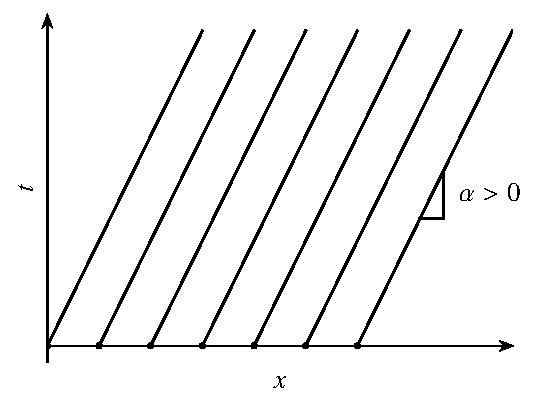
\includegraphics[width=0.5\linewidth]{Pictures/lsc_characteristics}
	\caption{Characteristic lines for the linear advection equation with $\alpha>0$ for different values of $x_0$.}
	\label{fig:linscal_charact}
\end{figure}

Consider $\alpha$ to be positive. The resulting characteristic curves are shown in Figure~\ref{fig:linscal_charact}. Observe that the slope of the curves is $\alpha$. Hence, we can find the value of $u$ at any point $(x,t)$ by tracing curves parallel to those in Figure~\ref{fig:linscal_charact}. We have characterized the behaviour of scalar hyperbolic equations. To analyze systems of equations, we must take into account additional considerations, which we explore in the next section.

\subsection{Linear Hyperbolic Systems}
\label{sec:linear_hyper_systems}
The advective components in our governing equations are responsible for the propagation of information from one point to another. In general, scalar conservation laws are simplifications of more complicated systems. Some of these systems are hyperbolic, which we can analyze as a superposition of advection equations with their corresponding wave speed. A system of $m$ equations
\begin{equation}
\frac{\partial \vec u}{\partial t} + A \frac{\partial \vec u}{\partial x} = 0,\quad \vec u = \begin{bmatrix} u_1 & u_2 & \ldots & u_m\end{bmatrix},
\label{eq:hyperprob_linearsystem}
\end{equation}
is said to be hyperbolic if the constant $m\times m$ matrix $A$, which is generally dense, has $m$ real distinct eigenvalues $\lambda_i$ and $m$ linearly independent eigenvectors $\vec q_i$. This can be written as the eigenvalue problem
\begin{equation}
	A \vec q_i = \lambda_i A,\quad i=1,2,\ldots,m,
\end{equation}
or in matrix form
\begin{equation}
	A Q = Q \Lambda,
	\label{eq:hyperprob_eigen}
\end{equation}
where $Q$ is the matrix of eigenvectors
\begin{equation}
	Q = 
	\begin{bmatrix}
		\vec q_1 & \vec q_2 & \ldots & \vec q_m
	\end{bmatrix}, \quad
\end{equation}
and $\Lambda$ is the diagonal matrix containing the eigenvalues of $A$
\begin{equation}
	\Lambda = 
	\begin{bmatrix}
		\lambda_1 	& 0			& \ldots  & 0 	   \\
		0	 		&  	\ddots  &         & \vdots \\
		\vdots 		&  		    & \ddots  & 0 \\
		0 			& \ldots	& 0		  & \lambda_m
	\end{bmatrix}.
\end{equation}
We have shown in the previous section that the scalar linear equation simply propagates information at a given characteristic speed, which represents the slope of the characteristic curves $x(t)$ in a space-time plane. In the case of a linear hyperbolic system, more than a single wave speed is embedded in the equations. Hence, multiple slopes are associated with any given $(x,t)$ point in the $x\times t$ plane, which are given by the eigenvalues of $A$. Now, how are these characteristic speeds related to $\vec u$? It turns out that the solution is considered to be a superposition of these waves. To illustrate this, the original system needs to be decoupled into $m$ independent equations. This is done by diagonalizing the constant matrix $A$.

Recall the $m$ eigenvectors of $A$ are linearly independent. Hence, we can transform Equation~\ref{eq:hyperprob_linearsystem} into \textit{characteristic form} by setting
\begin{equation}
	A = Q \Lambda Q^{-1}.
	\label{eq:A_diagonalize}
\end{equation}
Now, substituting A in Equation~\ref{eq:hyperprob_linearsystem} using~\ref{eq:A_diagonalize} and multiplying by $Q^{-1}$ yields
\begin{equation}
	Q^{-1} \frac{\partial \vec  u}{\partial t} + Q^{-1} Q \Lambda Q^{-1} \frac{\partial \vec u}{\partial t} = 0.
\end{equation}
For simplicity, define the vector of \textit{characteristic variables} $\vec \omega=Q^{-1} \vec{u}$. Hence, the characteristic form of hyperbolic system of PDEs is
\begin{eqBox}
\begin{equation}
	\frac{\partial \vec \omega}{\partial t} + \Lambda \frac{\partial \vec \omega}{\partial x} = 0.
\end{equation}
\end{eqBox}
We have now decoupled our original system into $m$ independent advection equations of the form
\begin{equation}
	\frac{\partial \omega_i}{\partial t} + \lambda_i \frac{\partial \omega_i}{\partial x} = 0,\quad i=1,\ldots,m,
\end{equation}
each of which has solution
\begin{equation}
	\omega_i = \omega_i^0(x-\lambda_i t),
\end{equation}
where the initial characteristic state can be found directly from the initial conditions by
\begin{equation}
	\vec{\omega}_0 = Q^{-1} \vec u_0. 
	\label{eq:initialstatetocharact}
\end{equation}
Similar to the scalar case, we can now draw characteristic curves in the $x\times t$ plane. These can be observed in Figure~\ref{fig:linsys_charact}, where we have considered the eigenvalues to be sorted 
\begin{equation}
	\lambda_1 < \lambda_2 < \ldots < \lambda_m.
\end{equation}
\begin{figure}[htbp]
	\centering
	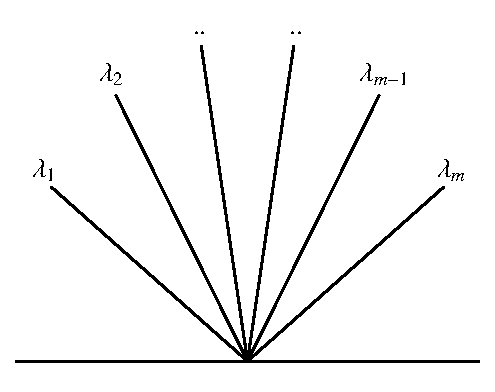
\includegraphics[width=0.5\linewidth]{Pictures/lsys_characteristics}
	\caption{Characteristic lines for a linear hyperbolic system of equations.}
	\label{fig:linsys_charact}
\end{figure}
We have now decomposed the vector of conserved quantities $\vec u$ into characteristic variables $\vec \omega$ employing the eigenvectors $\vec q_i$. Hence, the original variables can be recovered by coefficients $\omega_i$ and their corresponding eigenvector.
\begin{equation}
	u(x,t) = \sum_{i=1}^{m} \omega_i(x,t) \vec q_i=\sum_{i=1}^m \omega^0_i(x-\lambda_i t) \vec q_i.
	\label{eq:linsuperposition}
\end{equation}
\subsection{The Riemann Problem}
\subsubsection{The Scalar Case}
Consider the following initial-value problem (Figure~\ref{fig:scalar_riemann_u0}) for the scalar advection equation 
\begin{align}
	\frac{\partial u}{\partial t} + \alpha \frac{\partial u}{\partial x} = 0, \quad u(x,0) = 
	\begin{cases}
		u_L & \text{if}~x<0,\\
		u_R & \text{if}~x>0,\\
	\end{cases}
\end{align}
\begin{figure}[htbp]
	\centering
	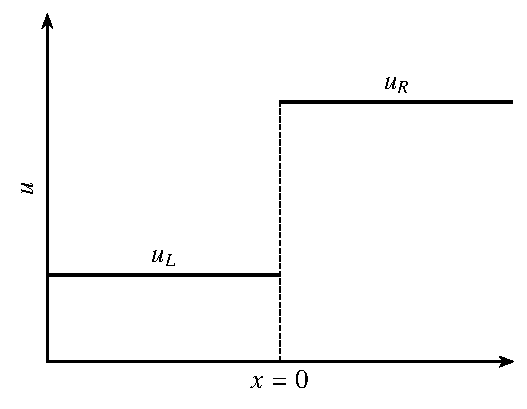
\includegraphics[width=0.5\linewidth]{Pictures/riem_lsc_u0}
	\caption{Scalar initial condition with discontinuity}
	\label{fig:scalar_riemann_u0}
\end{figure}
where $u_L$ and $u_R$ are piecewise constants and $u_L\neq u_R$. Based on our previous discussions, these constant values simply propagate along some characteristic curve in the $x\times t$ plane along with the discontinuity initially located at $x=0$. The characteristic line with the origin at this point defines the path of the discontinuity with equation $x=\alpha t$, as shown in Figure~\ref{fig:riem_charact_scalar}. Hence, on the left side of this curve, specifically where $x<\alpha t$, the solution is simply $u_L$, and on the right-hand side, where $x>\alpha t$, the solution is $u_R$. Hence, the Riemann solution to the scalar problem is simply
\begin{figure}[htbp]
	\centering
	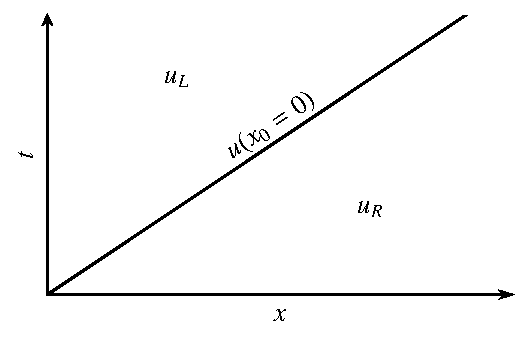
\includegraphics[width=0.5\linewidth]{Pictures/riem_lsc_characteristics}
	\caption{Characteristic line along which discontinuity propagates}
	\label{fig:riem_charact_scalar}
\end{figure}
\begin{eqBox}
\begin{equation}
	u(x,t) = 
	\begin{cases}
		u_L & \text{if}~x<\alpha t,\\
		u_R & \text{if}~x>\alpha t.\\
	\end{cases}
\end{equation}
\end{eqBox}
\subsubsection{Hyperbolic Systems}
Now consider the following initial-value problem, this time for a system of $m$ hyperbolic equations, where multiple values of the solution exist on each side of $x=0$
\begin{align}
	\frac{\partial \vec u}{\partial t} +A \frac{\partial \vec u}{\partial x} = 0, \quad \vec u(x,0) = 
	\begin{cases}
		\vec u_L & \text{if}~x<0,\\
		\vec u_R & \text{if}~x>0.\\
	\end{cases}
	\label{eq:ivp_linearsys}
\end{align}
Recall from Section~\ref{sec:linear_hyper_systems} that linear hyperbolic systems are driven by a superposition of multiple waves. To reveal these underlying advection equations, we must transform the original equations into characteristic form. From Equation~\ref{eq:initialstatetocharact}, we may write
\begin{equation}
	\vec \omega(x,0) = 
	\begin{cases}
		\vec \omega_L & \text{if}~x<0,\\
		\vec \omega_R & \text{if}~x>0,\\
	\end{cases}
	\label{eq:ivp_linearsys}
\end{equation}
where the $i$-th equation has solution
\begin{equation}
	\omega_i(x,t) = 
	\begin{cases}
		\omega_{L,i} &\text{if}~x<\lambda_i t, \\
		\omega_{R,i} &\text{if}~x>\lambda_i t. \\
	\end{cases}
\end{equation}
\begin{figure}[htbp]
	\centering
	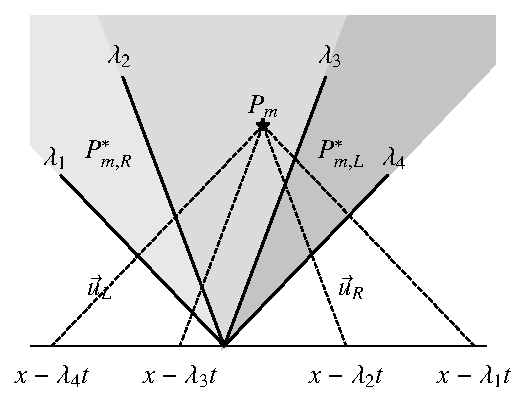
\includegraphics[width=0.5\linewidth]{Pictures/riem_lsys_characteristics}
	\caption{Characteristic curves for the Riemann problem with $m=4$. Note the value of the maximum sub-index changes for each point $P$. For $P_{m,L}^*$, $I=1$, for $P_{m}$, $I=2$ and for $P_{m,R}^*$, $I=3$. (Adapted from~\cite{levequeFiniteVolumeMethods2002})}
	\label{fig:characteristics_riemann}
\end{figure}
The eigenvalues of $A$ can be observed in Figure~\ref{fig:characteristics_riemann} for the case of $m=4$ equations. Now, suppose you have a set of coordinates $(x,t)$ where you want to know the value of the solution. At any point in the $x\times t$ domain, the solution only depends on $u(x,0)=u(x_0)=u_0$. Hence, we can determine the value of $\vec u$ at any point by drawing lines parallel to the characteristic curves. On the left of $\lambda_1$, tracing parallel lines only yields initial values which correspond to the left state $\vec u_L$, hence the solution can be computed by
\begin{equation}
	\vec u_L = \sum_{i=1}^m  \omega_{L,i} \vec q_i.
\end{equation}
Similarly, at any point on the right side of $\lambda_m$ ($\lambda_4$ in Figure~\ref{fig:characteristics_riemann}) we find
\begin{equation}
	\vec u_R = \sum_{i=1}^m  \omega_{R,i} \vec q_i.
\end{equation}
Now, what if we are interested in finding the solution at the point $P_m$ in Figure~\ref{fig:characteristics_riemann}?. Tracking the solution back to its initial value shows that values of $x-\lambda t$ are located on both the left and right-hand sides of $x=0$. Hence, we require a combination of both left and right states. Note that at any point within the region defined by $\lambda_2$ and $\lambda_3$, the solution $\vec u_m$ depends on the linear combination of left and right states. Moving $P_m$ to the left or right of these characteristic lines, for example where points $P_{m,L}^*$ and $P_{m,R}^*$ are will require a different combination $\vec \omega_L$ and $\vec\omega_R$. Hence, to generalize the equation for the solution at any point, define $I^*=I^*(x,t)$ to be the maximum index $i$ for which $x>\lambda_i t$.  Then, the solution can be found by
\begin{equation}
	\vec u_m = \sum_{i=I^*+1}^m \omega_{L,i} \vec q_i + \sum_{i=1}^{I^*} \omega_{R,i} \vec q_i.
	\label{eq:riemann_solution}
\end{equation}
Since the solution is constant along each characteristic line, the jump between two states is also constant and is given for the whole system
\begin{equation}
	\vec \delta = Q^{-1}(\vec u_R - \vec u_L). 
	\label{eq:lin_rankinehugoniot}
\end{equation}
Hence the jump across the $\lambda_i$-characteristic is given by $\delta_i = \omega_{R,i}-\omega_{L,i}$, which is known as the strength of the $i$-th wave. Note that Equation~\ref{eq:lin_rankinehugoniot} is called the \textit{Rankine-Hugoniot} condition, and will be useful for the analysis of nonlinear problems later in this chapter.
\subsubsection{Example case: Linear Acoustics}
Consider the propagation of sound waves in a motionless gas. Small changes in pressure and density propagate in the surrounding air. This propagation is governed in one dimension by
\begin{equation}
	\begin{bmatrix}
		\rho \\ \rho v 
	\end{bmatrix}_t
	+
	\begin{bmatrix}
		\rho v \\ \rho v^2 + p(\rho)
	\end{bmatrix}_x
	= 0.
	\label{eq:massmomentum_acoustics}
\end{equation}
These are the Euler equations, one of which is the nonlinear PDE for the conservation of momentum. This system can be written in \textit{quasilinear} form~\cite{toroRiemannSolversEvolved2006}
\begin{equation}
	\frac{\partial \vec u}{\partial t} + \vec {f^\prime}(\vec u) \frac{\partial \vec u}{\partial x} = 0,
\end{equation}
where
\begin{align}
	\vec u &= 
	\begin{bmatrix}
		\rho \\ \rho v
	\end{bmatrix}
	=
	\begin{bmatrix}
		u_1 \\ u_2
	\end{bmatrix},
	\\
	\vec F(\vec u) &= 
	\begin{bmatrix}
		\rho v \\ \rho v^2 + p(\rho)
	\end{bmatrix}
	=
	\begin{bmatrix}
		u_2 \\ \frac{u_2^2}{u_1^2} + p(u_1)
	\end{bmatrix}.
\end{align}
Then $A = \vec {f^\prime} (\vec u)$ is the Jacobian matrix and is given by
\begin{equation}
	A = \vec {f^\prime} (\vec u) =
	\begin{bmatrix}
		\frac{\partial f_1}{\partial u_1} & \frac{\partial f_1}{\partial u_2} \\ 
		\frac{\partial f_2}{\partial u_1} & \frac{\partial f_2}{\partial u_2} 
	\end{bmatrix}
	= 
	\begin{bmatrix}
		0 & 1 \\
		-\frac{u_2^2}{u_1^2} + p^\prime(u_1) & \frac{2 u_2}{u_1}
	\end{bmatrix}
	=
	\begin{bmatrix}
		0 & 1 \\
		-v^2 + p^\prime(\rho) & 2 v
	\end{bmatrix}.
\end{equation}
We can analyze systems with small disturbances by linearizing about some state. This can be done by considering the flow properties to be the sum of an initial variable plus a perturbation term
\begin{align}
	u &= \tilde u(x,t), \\
	\rho &= \rho_0 + \tilde \rho(x,t), \\
	p & = p_0 + \tilde p(x,t),
\end{align}
and since the gas is considered motionless, we have set $u_0=0$. Neglecting products of small disturbances and applying the chain rule to the momentum equations, the linear system can be written 
\begin{eqBox}
\begin{equation}
	\begin{bmatrix}
		\tilde \rho \\  \tilde u
	\end{bmatrix}_t 
	+ \begin{bmatrix}
		0 & \rho_0 \\
		\frac{c^2}{\rho_0} & 0 \\
	\end{bmatrix}
	\begin{bmatrix}
		\tilde \rho \\  \tilde u
	\end{bmatrix}_x
	= 0,
	\label{eq:linearized_gasdyn}
\end{equation}
\end{eqBox}
where $c=\sqrt{p'(\rho_0)}$ is the speed of sound. Now, consider the following Riemann problem
\begin{equation}
	\vec u(x,0) = \vec u_0 = 
	\begin{cases}
		\vec u_L & \text{if }x<0, \\
		\vec u_R & \text{if }x>0,\\
	\end{cases}
\end{equation}
where $\vec u_L = \begin{bmatrix} \rho_L & u_L \end{bmatrix}^T$ and $\vec u_R = \begin{bmatrix} \rho_R & u_R \end{bmatrix}^T$, $\vec u_L \neq \vec u_R$. Note that the problem is linear due to the above procedure. We can compute the eigenvalues of $A$ in Equation~\ref{eq:linearized_gasdyn} by setting
\begin{equation}
	\det(A-I\lambda) = 0,
\end{equation}
where $I$ is the identity matrix. Solving the eigenvalue problem yields the characteristic polynomial 
\begin{equation}
	\lambda^2 - c^2 = 0,
\end{equation}
which has solutions 
\begin{align}
	\lambda_1 = -c, \quad
	\lambda_2 = +c.
\end{align}
The corresponding matrix of eigenvectors can be found to be
\begin{align}
	Q = 
	\begin{bmatrix}
		\rho_0 & \rho_0 \\
		-c & c
	\end{bmatrix},
\end{align}
with inverse
\begin{align}
	Q^{-1}= 
	\frac{1}{2\rho_0 c}
	\begin{bmatrix}
		c & -\rho_0 \\
		c & \rho_0
	\end{bmatrix}.
\end{align}
\begin{figure}[htbp]
	\centering
	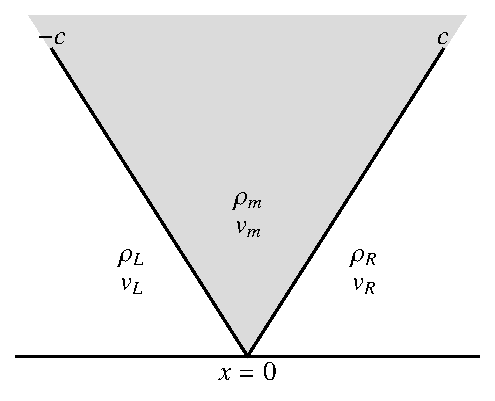
\includegraphics[width=0.5\linewidth]{Pictures/riem_linacoustics_characteristics}
	\caption{Characteristic curves for the linear acoustics example}
	\label{fig:acoustics_charact}
\end{figure}
As we expected, the solution consists of a superposition of left-going and right-going sound waves, which represent the slopes of the characteristic lines shown in Figure~\ref{fig:acoustics_charact}. Now, we analyze the characteristic form of Equation~\ref{eq:linearized_gasdyn} seeking a Riemann solution $\vec u_m$. Note that for systems of $m=2$ equations, the Riemann state only depends on the single region highlighted in Figure~\ref{fig:acoustics_charact}. We start by finding the values of $\vec \omega_L$ and $\vec \omega_R$ by
\begin{equation}
	\vec \omega_L = 
	\begin{bmatrix}
		\omega_{L,1} \\ \omega_{L,2}
	\end{bmatrix}
	= Q^{-1} \vec v_L = \frac{1}{2c\rho_0}
	\begin{bmatrix}
		c & -\rho_0 \\
		c & \rho_0 
	\end{bmatrix}
	\begin{bmatrix}
		\rho_L \\ v_L
	\end{bmatrix}.
\end{equation}
Hence
\begin{align}
	\omega_{L,1} &= \frac{c \rho_L - \rho_0 v_L}{2 c \rho_0}, \\
	\omega_{L,2} &= \frac{c \rho_L + \rho_0 v_L}{2 c \rho_0}.
\end{align}
Similarly, for the right state we can find
\begin{align}
	\omega_{R,1} &= \frac{c \rho_R - \rho_0 v_R}{2 c \rho_0}, \\
	\omega_{R,2} &= \frac{c \rho_R + \rho_0 v_R}{2 c \rho_0}.
\end{align}
In Equation~\ref{eq:riemann_solution}, $I^*=1$, hence
\begin{equation}
	\vec u_m = 
	\begin{bmatrix}
		\rho_m \\ v_m
	\end{bmatrix} =  \sum_{i=2}^2 \omega_{L,i} \vec q_i + \sum_{i=1}^{1} \omega_{R,i} \vec q_i = 
	\omega_{L,2} \vec q_2 + \omega_{R,1} \vec q_1,
\end{equation}
which yields the exact Riemann solution for the linear acoustics equation
\begin{eqBox}
	\begin{align}
		\rho_m &= \frac{1}{2} (\rho_R+\rho_L) + \frac{1}{2}\frac{\rho_0}{c} (u_L-u_R), \\
		u_m &= \frac{1}{2}\frac{c}{\rho_0}(\rho_L-\rho_R) + \frac{1}{2} (u_R+u_L).
		\label{eq:riemann_solution_acoustics}
	\end{align}
\end{eqBox}
Similar to~\cite{toroRiemannSolversEvolved2006}, we can define the values of $\rho_0=1$, $c=1$ and given the initial left and right states
\begin{equation}
	\vec u_L = 
	\begin{bmatrix}
		\rho_L \\ v_L
	\end{bmatrix}
	 = 	
	 \begin{bmatrix}
		0.5 \\ 0
	\end{bmatrix},
	\quad
	\vec u_R = 
	\begin{bmatrix}
		\rho_R \\ v_R
	\end{bmatrix}
	 = 	
	 \begin{bmatrix}
		0.25 \\ 0.0
	\end{bmatrix},
\end{equation}
as shown in Figure~\ref{fig:riem_acoustics_example_u0}, we can determine the middle state from Equation~\ref{eq:riemann_solution_acoustics}. Hence $\rho_m=0.375$ and $v_m=0.125$. Results can be seen in Figure~\ref{fig:riem_acoustics_example_sol}, where a symmetric wave can be seen to have moved from $x=0$ to $-ct$ and $ct$ for the left and right discontinuities, respectively. 
\begin{figure}[htbp]
	\centering
	\begin{subfigure}[b]{0.49\textwidth}
		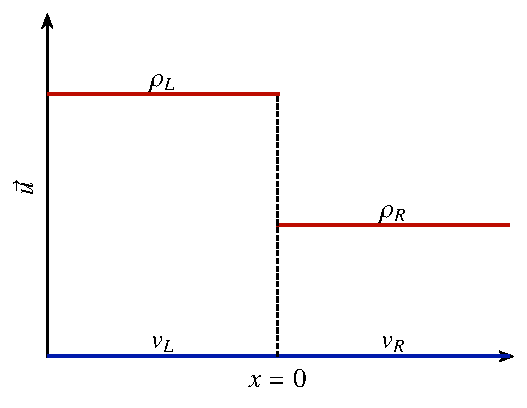
\includegraphics[width=\linewidth]{Pictures/riem_linacoustics_u0}
		\caption{Initial condition}
		\label{fig:riem_acoustics_example_u0}
	\end{subfigure}
	\begin{subfigure}[b]{0.49\textwidth}
		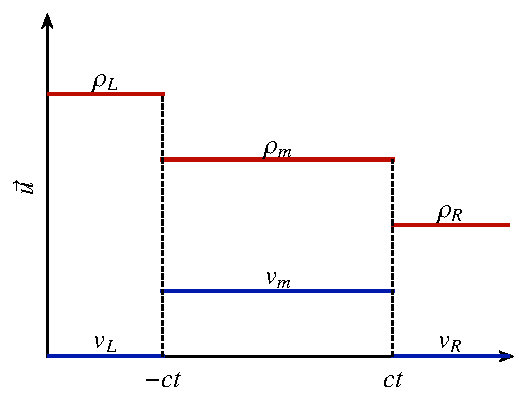
\includegraphics[width=\linewidth]{Pictures/riem_linacoustics_sol}
		\caption{Solution at $t>0$}
		\label{fig:riem_acoustics_example_sol}
	\end{subfigure}
	\caption{Example solution with values for the linear acoustics case.}
	\label{fig:riem_acoustics_example}
\end{figure}
\section{Nonlinear Hyperbolic Problems}
Consider the following one-dimensional scalar conservation law
\begin{equation}
	\frac{\partial u}{\partial t} + \frac{\partial f(u)}{\partial x} = 0,
\end{equation}
where $f(u)$ is the flux. In Section~\ref{sec:linear_hyperb_problems}, we analyzed a flux function of the form $f(u)=\alpha u$, corresponding to linear advection. In this section, we consider a nonlinear flux function of the form $f(u)=\frac{1}{2} u^2$, which leads to the inviscid Burgers equation. For this type of problem, $u$ is expected not only to translate but also to deform towards the formation of shocks. Similar to Section~\ref{sec:linear_hyperb_problems}, we want to analyze the behaviour of this PDE via the method of characteristics. Hence, we write the \textit{quasilinear form} of Burgers' equation
\begin{equation}
	\frac{\partial u}{\partial t} + f'(u)\frac{\partial u}{\partial x} = 0,
	\label{eq:nonconserv_burgers}
\end{equation}
where $f'(u) = u$. Recall that in the $x-t$ plane, we look for lines along which the solution remains unchanged. Using the chain rule for $u(x(t), t)$, we obtain
\begin{equation}
	\frac{du}{dt} = \frac{\partial u}{\partial t} + \frac{dx}{dt}\frac{\partial u}{\partial t} = 0.
	\label{eq:chainrule_burgers}
\end{equation}
Furthermore, comparing Equations~\ref{eq:chainrule_burgers} and~\ref{eq:nonconserv_burgers}, we observe that
\begin{equation}
	\frac{dx}{dt} = u,
\end{equation}
which allows us to obtain an equation for the characteristic line that passes through $x_0$
\begin{equation}
	x = x_0 + u_0 t,
	\label{eq:charact_burgers}
\end{equation}
where $u_0=u(x,0)$ is the slope of each line. This means that each characteristic line has an inclination that depends on the initial value of the solution. Note that since $u$ is the characteristic speed of the problem and $f(u)$ is an increasing function, i.e. higher values of the solution travel faster than smaller values of $u$, causing the solution to deform. To illustrate this, consider the following example shown in Figure~\ref{fig:nslcexa}
\begin{equation}
	u(x,0) = 
	\begin{cases}
		1 & \text{if}~x < 0,\\
		1-x & \text{if}~0<x<1, \\ 
		0 & \text{if}~x>1.
	\end{cases}
	\label{eq:nlscex0}
\end{equation}

\begin{figure}[htbp]
	\centering
	\begin{subfigure}[b]{0.49\linewidth}
	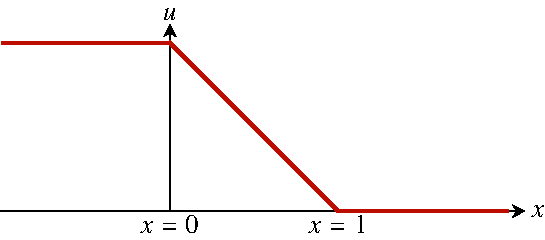
\includegraphics[width=\linewidth]{Pictures/nonlinear_scalar_example_u0}
	\caption{$u(x,0)$}
	\label{fig:nslcexa}
	\end{subfigure}
	\begin{subfigure}[b]{0.49\linewidth}
		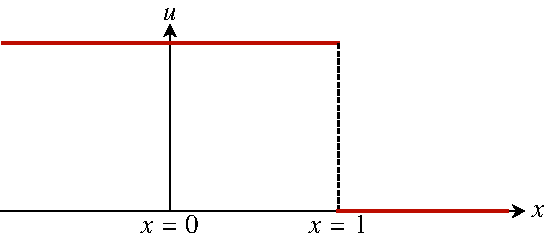
\includegraphics[width=\linewidth]{Pictures/nonlinear_scalar_example_uf}
		\caption{$u(x,1)$}
	\label{fig:nslcexb}
	\end{subfigure}
	\caption{Solution at $t=0$ and $t=1$ for Equation~\ref{eq:nlscex0}}
	\label{fig:nslcex}
\end{figure}

Since the solution is its own convective speed, we expect the region $x<1$ to move towards the right, and the region after this point to remain stationary. Then a portion of the initial solution will meet at $x=1$, where a shock will form. Let us now visualize this via the method of characteristics. Using Equation~\ref{eq:charact_burgers} at different $x$-locations, we draw the characteristic lines in Figure~\ref{fig:nlscchar}. Multiple curves can be seen to intersect for a single value of $u$ at $(x,t) = (1,1)$, corresponding to the solution illustrated in Figure~\ref{fig:nslcexb} at $t=1$. 
\begin{figure}[htbp]
	\centering
	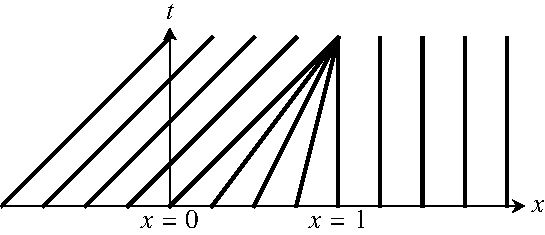
\includegraphics[width=0.45\linewidth]{Pictures/nonlinear_scalar_characteristics}
	\caption{Characteristic lines for Equation~\ref{eq:nlscex0}.}
	\label{fig:nlscchar}
\end{figure}

At $t=1$, the method of characteristics breaks. To ensure conservation after this moment, the discontinuity is expected only to translate at a speed $s$. This speed depends on the values of both sides of the discontinuity and can be obtained via the Rankine-Hugoniot relation, which we now derive. 

Consider the integral form of the conservation law applied to a finite region in the $(x,t)$ plane where the shock has already formed and only translates, similar to Figure~\ref{fig:riem_charact_scalar}. This results in
\begin{equation}
	\frac{\partial}{\partial t} \int_{x_L}^{x_R} u(x,t) dx + [f(u_R) - f(u_L)] = 0.
	\label{eq:integral_cl_rankinehugoniot}
\end{equation}
Assuming constant values of $u$ on the left and right side of the discontinuity, we can rewrite Equation~\ref{eq:integral_cl_rankinehugoniot}
\begin{equation}
	\frac{u(x_R,t)-u(x_L,t)}{\Delta t} \Delta x + f(u_R)-f(u_L) = 0,
\end{equation}
which in the limit of $\Delta t\rightarrow 0$ becomes
\begin{eqBox}
	\begin{equation}
		s = \frac{dx}{dt} = \frac{f(u_R)-f(u_L)}{u_R-u_L},
	\end{equation}
\end{eqBox}
where $s$ is the shock speed. This equation is known as the Rankine-Hugoniot relation. For the Burgers equation with $f(u)=u^2/2$, we find that the shock speed is given by
\begin{equation}
	s = \frac{1}{2} \frac{\left(u_R^2 - u_L^2\right)}{u_R-u_L} = \frac{1}{2} \left(u_L + u_R\right),
\end{equation}
which can be computed for the problem in Equation~\ref{eq:nlscex0} to be $s=\frac{1}{2}\left(0+1\right)=\frac{1}{2}$. 
\subsubsection{Weak solutions}
Now, consider the following initial conditions
\begin{equation}
	u(x,0) = 
	\begin{cases}
		0 & \text{if}~x < 0,\\
		1 & \text{if}~x > 0. 
	\end{cases}
	\label{eq:nlscex00}
\end{equation}
In this case, the characteristic lines do not intersect and are displayed in Figure~\ref{fig:nlscex2}. 
\begin{figure}[htbp]
	\centering
	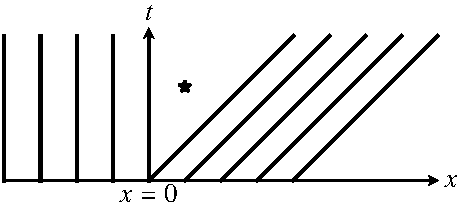
\includegraphics[width=0.4\linewidth]{Pictures/nonlinear_scalar_entropycond_0}
	\caption{Characteristic lines for Equation~\ref{eq:nlscex00}.}
	\label{fig:nlscex2}
\end{figure}
While these curves do not cross, we are missing information in the star region.  One possible solution of this problem can be written
\begin{equation}
	u(x,t) = 
	\begin{cases}
		0 & \text{if}~x < t/2,\\
		1 & \text{if}~x > t/2,
	\end{cases}
	\label{eq:nlscsol1}
\end{equation}
as illustrated in Figure~\ref{fig:expansionshock}. This form of the solution satisfies the Rankine-Hugoniot relation and is known as an expansion shock, where information appears to come out of a discontinuity. From a physical point of view, this violates the entropy condition. In a physical shock wave, characteristics are expected to go into the discontinuity as time advances. Hence, while Equation~\ref{eq:nlscsol1} is a mathematical solution, it is not an entropy or physically relevant solution. 
\begin{figure}[tb]
	\centering
	\begin{subfigure}[b]{0.4\linewidth}
		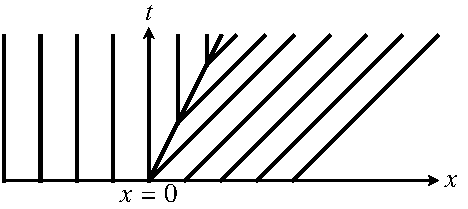
\includegraphics[width=\linewidth]{Pictures/nonlinear_scalar_entropycond_1}
	\caption{Expansion shock}
	\label{fig:expansionshock}
	\end{subfigure}
	~
	\begin{subfigure}[b]{0.4\linewidth}
		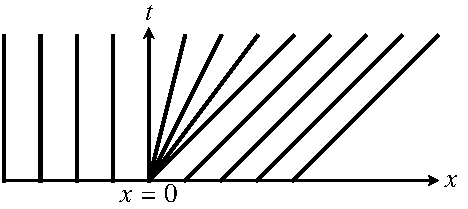
\includegraphics[width=\linewidth]{Pictures/nonlinear_scalar_entropycond_2}
		\caption{Rarefaction fan}
	\label{fig:rarefactionfan}
	\end{subfigure}
	\caption{Mathematically admissible solutions to problem in Equation~\ref{eq:nlscex00}}
	\label{fig:entropycond}
\end{figure}

Consider instead 
\begin{equation}
	u(x,t) = 
	\begin{cases}
		0 & \text{if}~x \leq t/2,\\
		\frac{x}{t} & \text{if}~0 \leq x \leq t, \\
		1 & \text{if } x \geq t,
	\end{cases}
	\label{eq:nlscsol1}
\end{equation}
which is known as a rarefaction wave, shown in Figure~\ref{fig:rarefactionfan}. In this case, the solution consists of a smooth transition between the left and right states, consistent with the entropy condition.

Even with smooth initial conditions, nonlinear equations can develop discontinuities. For a general conservation law, we say a solution that satisfies a PDE of order $k$ is a classical solution if the first $k$ derivatives exist and are continuous. So, how is a discontinuous solution admitted in a PDE? It turns out that we need to expand the range of admissible solutions to include those that may not be differentiable so that we can deal with the formation of shocks. The set of both classical and discontinuous $u$ is generally known as weak solutions. They are considered to satisfy the conservation law in an integral sense, which was the approach that we used to derive the Rankine-Hugoniot relation.

Recall our second example in Equation~\ref{eq:nlscex00}. We showed that weak solutions are not necessarily unique, and hence we must add a constraint to single out those relevant in the physical world. Hence, to identify physical solutions, we consider a discontinuity to be a physical shock wave only if the following entropy condition is satisfied 
\begin{equation}
	f'(u_L) > s > f'(u_R),
\end{equation}
which is consistent with the choice of Equation~\ref{eq:nlscsol1} as the physically relevant solution in our second example.

\subsection{Nonlinear Hyperbolic Systems}
Applications of engineering interest can be described by a system of conservation laws of the form
\begin{equation}
	\frac{\partial \vec u}{\partial t} + \frac{\partial \vec F (\vec u)}{\partial x} = 0,
	\label{eq:9348342432}
\end{equation}
where $\vec u$ is the vector of conserved variables and $\vec F(\vec u)$ is the vector of fluxes. Previously, we considered constant Jacobian matrices that led to a set of linear equations. In this section, we consider problems whose Jacobian matrices have the form 
\begin{equation}
	A(\vec u) = \frac{\partial \vec F(\vec u)}{\partial \vec u},
\end{equation}
and hence both the eigenvalues and eigenvectors depend on the value of the solution, which in turn depends on time. An example of a nonlinear hyperbolic system is given by the Euler equations, which can be written in one dimension using Equation~\ref{eq:9348342432} with
\begin{equation}
	\vec u = \begin{bmatrix}
		u_1 \\ u_2 \\ u_3
	\end{bmatrix}
	= 
	\begin{bmatrix}
		\rho \\ \rho v \\ \rho E
	\end{bmatrix},
	\quad\quad
	\vec F = 
	\begin{bmatrix}
		f_1 \\ f_2 \\ f_3
	\end{bmatrix}
	= 
	\begin{bmatrix}
		\rho v \\ \rho v^2 + P \\ v(\rho E + p)
	\end{bmatrix}.
\end{equation}
$\rho$ is density, $v$ is velocity and $E$ is the specific energy
\begin{equation}
E = e + \frac{1}{2}v^2.
\end{equation}
We assume ideal gas law, hence the specific internal energy $e$ is given by
\begin{equation}
	e = \frac{p}{(\gamma-1)\rho},
\end{equation}
where $\gamma$ is the ratio of specific heats. In quasilinear form, we write 
\begin{equation}
	\frac{\partial \vec u}{\partial t} + A(\vec u) \frac{\partial \vec u}{\partial x} = 0,
\end{equation}
where $A(\vec u)$ is the Jacobian matrix given by
\begin{equation}
	A(\vec u) = \frac{\partial \vec F(\vec u)}{\partial \vec u} =
	\begin{bmatrix}
	\frac{\partial f_1}{\partial u_1} & \frac{\partial f_1}{\partial u_2} & \frac{\partial f_1}{\partial u_3} \\
	\frac{\partial f_2}{\partial u_1} & \frac{\partial f_2}{\partial u_2} & \frac{\partial f_2}{\partial u_3} \\
	\frac{\partial f_3}{\partial u_1} & \frac{\partial f_3}{\partial u_2} & \frac{\partial f_3}{\partial u_3} \\
	\end{bmatrix},
\end{equation}
To compute $A(\vec u)$, we write the Euler fluxes in terms of $u_1,~u_2,~u_3$
\begin{equation}
	\vec F = 
	\begin{bmatrix}
		f_1 \\ f_2 \\ f_3
	\end{bmatrix}
	= 
	\begin{bmatrix}
		u_2 \\ u_2^2/u_1 + (\gamma-1)(u_3-u_2^2/2 u_1) \\ u_3 \frac{u_2}{u_1} \gamma - \frac{u_2^3}{u_1^2}\frac{(\gamma-1)}{2} 
	\end{bmatrix}.
\end{equation}
Hence, the Jacobian matrix for the Euler equations is given by
\begin{align}
	A(\vec u) = 
	\begin{bmatrix}
		0 & 1 & 0 \\
		\frac{1}{2}(3-\gamma)\left(\frac{u_2}{u_1}\right)^2 & (3-\gamma)\left(\frac{u_2}{u_1}\right) & \gamma-1 \\
		(\gamma-1) \left(\frac{u_2}{u_1}\right)^3 - \gamma \frac{u_2 u_3}{u_1^2} & \gamma \frac{u_3}{u_1}-\frac{3}{2}(\gamma-1)\left(\frac{u_2}{u_1}\right)^2 & \gamma \frac{u_2}{u_1}
	\end{bmatrix},
\end{align}
or using the conserved variables
\begin{eqBox}
	\begin{align}
		A(\vec u) = 
		\begin{bmatrix}
			0 & 1 & 0 \\
			\frac{1}{2} (\gamma-3)v^2 & (3-\gamma)v & \gamma-1 \\ 
			\frac{1}{2} (\gamma-2) v^3 - c^2 \frac{v}{\gamma-1} & \frac{3-2\gamma}{2}v^2 + \frac{c^2}{\gamma-1} & \gamma v
		\end{bmatrix},
		\label{eq:eulerjacobian}
	\end{align}
\end{eqBox}
where $c$ is the speed of sound
\begin{equation}
	c = \sqrt{\frac{\gamma p}{\rho}}.
\end{equation}
The eigenvalues of $A(\vec u)$ are 
\begin{equation}
	\lambda_1 = v - c, \quad\quad \lambda_2 = v, \quad\quad \lambda_3 = v + c,
\end{equation}
and the associated eigenvectors are 
\begin{equation}
	\vec q_1 = \begin{bmatrix}
		1 \\ v - c \\ H - vc
	\end{bmatrix},
	\quad\quad
	\vec q_2 = \begin{bmatrix}
		1 \\ v \\ \frac{v^2}{2}
	\end{bmatrix},
	\quad\quad
	\vec q_3 = \begin{bmatrix}
		1 \\ v + c \\ H + vc
	\end{bmatrix},
\end{equation}
where $H$ is the total enthalpy defined as
\begin{equation}
	H = E + \frac{p}{\rho}.
\end{equation} 
The eigenvalues of the Euler system are distinct, and a complete set of eigenvectors can be found, proving that the Euler equations are strictly hyperbolic. The eigenvalues represent the characteristic speeds of the problem,  showing that the Euler equations can be interpreted as a superposition of a left-travelling sound wave, a momentum wave and a right-going sound wave, consistent with the propagation of sound. The nonlinearity of these equations makes the study of the Riemann problem much more challenging compared to the linear systems. In the next section, we briefly discuss some important considerations when analyzing the Riemann problem for the Euler equations.
\subsection{The Riemann Problem for the Euler equations}
Consider a tube with a thin membrane at $x=0$ separating two different gases, each with a given density $\rho$ velocity $v$, and pressure $p$ as shown in Figure~\ref{fig:shocktube}.  Initially, both gases are considered at rest ($v_L=v_R=0$). Note it can also be the same gas at different pressures. At time $t$, the thin membrane is ruptured, causing the fluid in the region of high pressure to move towards the low-pressure side to reach thermodynamic equilibrium. This configuration is known as \textit{Sod's shock tube} and is the physical equivalent to the Riemann problem in gas dynamics~\cite{toroRiemannSolversEvolved2006}.
\begin{figure}[htbp]
	\centering
	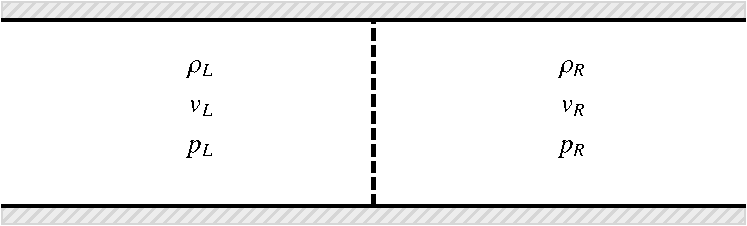
\includegraphics[width=0.6\linewidth]{Pictures/sod_shock_tube}
	\caption{Sod's shock-tube problem}
	\label{fig:shocktube}
\end{figure}

It can be shown that the solution to this problem consists of a contact discontinuity associated with $\lambda_2$, and a shock or a rarefaction wave associated with $\lambda_1$ and $~\lambda_3$. Four different configurations are then possible solutions for the Riemann problem~\cite{toroRiemannSolversEvolved2006}, all of which need to be considered when deriving an exact solution. These are shown in Figure~\ref{fig:euler_characteristics}.
\begin{figure}[htb]
	\centering
	\begin{subfigure}[b]{0.35\linewidth}
		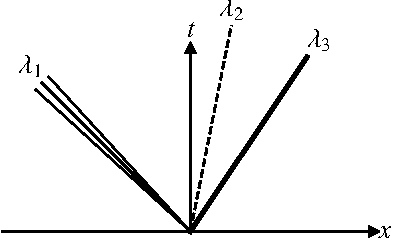
\includegraphics[width=\linewidth]{Pictures/euler_characteristics_0.pdf}
		\caption{}
	\end{subfigure}~
	\begin{subfigure}[b]{0.35\linewidth}
		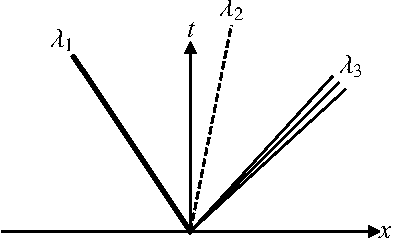
\includegraphics[width=\linewidth]{Pictures/euler_characteristics_1.pdf}
		\caption{}
	\end{subfigure} \\
	\begin{subfigure}[b]{0.35\linewidth}
		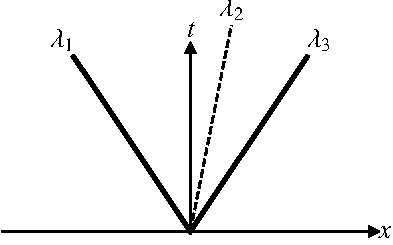
\includegraphics[width=\linewidth]{Pictures/euler_characteristics_2.pdf}
		\caption{}
	\end{subfigure}~
	\begin{subfigure}[b]{0.35\linewidth}
		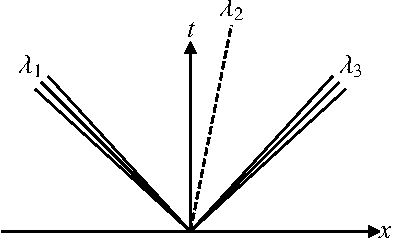
\includegraphics[width=\linewidth]{Pictures/euler_characteristics_3.pdf}
		\caption{}
	\end{subfigure}
	\caption{Possible characteristic configurations for the Euler Riemann problem}
	\label{fig:euler_characteristics}
\end{figure}

Solving the exact Riemann problem for the Euler equations turns out to be very expensive and requires the use of iterative methods to find the pressure between the left and right states. We refer the reader to \cite{levequeFiniteVolumeMethods2002,toroRiemannSolversEvolved2006} for a detailed derivation of the exact solution.
\subsubsection{Example}
To visualize the behaviour of the Euler equations, consider Sod's shock tube problem with initial conditions
\begin{align}
	\vec u_L = 
	\begin{bmatrix}
		\rho_L \\ v_L \\ p_L 
	\end{bmatrix}
	= 
	\begin{bmatrix}
		1 \\ 0 \\ 1
	\end{bmatrix},
	\quad \text{and} \quad 
	\vec u_R = 
	\begin{bmatrix}
		\rho_R \\ v_R \\ p_R
	\end{bmatrix}
	= 
	\begin{bmatrix}
		\frac{1}{8} \\ 0 \\ \frac{1}{10}
	\end{bmatrix}.
\end{align}
After $t=0.2$, the exact solution can be seen in Figure~\ref{fig:shocktubesol}. The figures are divided into five regions, which we denote A, B, C, D, E, from left to right. 
\begin{figure}[htbp]
	\centering
	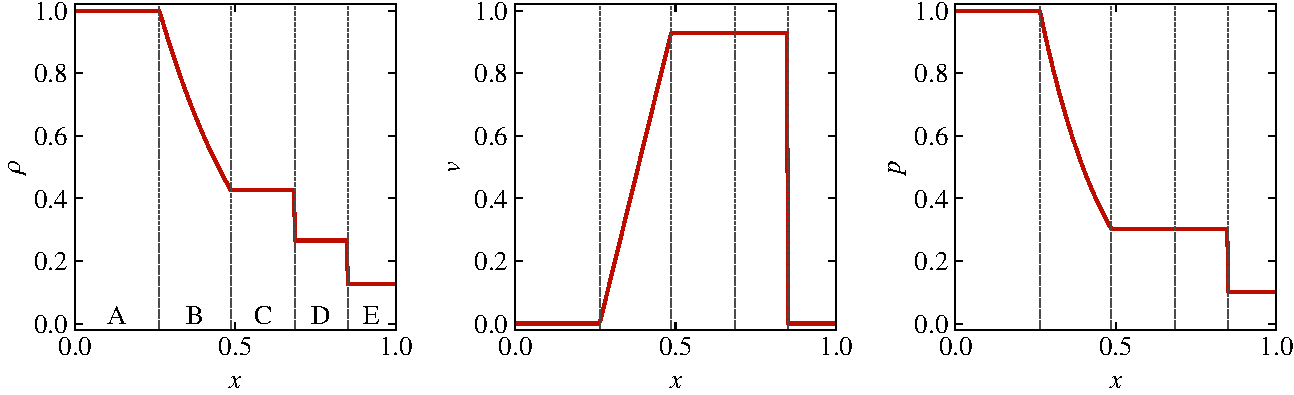
\includegraphics[width=\linewidth]{Pictures/sod_shock_tube_solution}
	\caption{Exact solution to Sod's shock tube problem at $t=0.2$}
	\label{fig:shocktubesol}
\end{figure}
\begin{itemize}
	\item Regions A and E contain the initial left and right states, respectively.
	\item Region B consists of a rarefaction wave, which is a smooth transition of quantities $\rho,~v,$ and $p$. 
	\item At the interface between regions C and D, we observe a contact discontinuity. This wave represents the effects of the initial separation of the left and right states travelling to the region of low pressure. Across this wave, pressure and velocity remain constant, but density is discontinuous.
	\item At the interface between regions D and E, a shock wave has formed due to the nonlinearities of the Euler equations. This shock wave travels with a speed $s$, which satisfies the Rankine-Hugoniot relationship. In this case, all considered quantities $\rho,~v$ and $p$ present discontinuous behaviour across the wave. 
\end{itemize}

\subsection{A Riemann Solver for the Euler Equations}
A more cost-effective approach is the use of approximate Riemann solvers to compute the behaviour of the left and right states of interfaces in finite volume schemes. In this section, we discuss the Riemann solver of Roe. Recall the quasilinear form of a conservation law
\begin{equation}
	\frac{\partial \vec u}{\partial t} + A(\vec u) \frac{\partial \vec u}{\partial x} = 0.
	\label{eq:09707}
\end{equation}
For the Euler equations, $A(\vec u)$ is given by Equation~\ref{eq:eulerjacobian}. The eigenvalues of $A$ depend on the value of the solution and hence vary in time. Recall that for the Euler equations, three types of waves can be expected: contact, rarefaction and shock waves. We are interested in handling the formation of the shocks.  Consider the following finite volume scheme with the forward Euler time-stepping method
\begin{equation}
	\vec u^{t+1}_i = \vec u^t_i - \frac{\Delta t}{\Delta x} \left[\vec F_{i+1/2} - \vec F_{i-1/2}\right],
\end{equation}
where $\vec F_{i-1/2}$ and $\vec F_{i+1/2}$ are interface fluxes on the left and right sides of the cell, respectively, and are defined such that
\begin{align}
	\vec F_{i-1/2} &= \vec F (\vec u_{i-1/2}), \\
	\vec F_{i+1/2} &= \vec F (\vec u_{i+1/2}).
\end{align}
Hence, at the interfaces, we need to solve a Riemann problem of the form
\begin{align}
	\frac{\partial \vec u}{\partial t} + \frac{\partial \vec F}{\partial x} &= 0,\\
	\vec u(x, 0) &=
	\begin{cases}
		\vec u_L & \text{if } x<0,\\
		\vec u_R & \text{if } x>0.
	\end{cases}
\end{align}
Roe proposed considering instead a constant Jacobian matrix $\tilde A$ with the following properties~\cite{toroRiemannSolversEvolved2006}
\begin{itemize}
	\item $\tilde A$ must have real eigenvalues and a complete set of eigenvectors such that the problem in Equation~\ref{eq:09707} is hyperbolic.
	\item $\tilde A$ must be consistent with the exact problem, i.e. $\tilde A (\vec u, \vec u) = A(\vec u)$.
	\item The resulting system must be conservative across discontinuities, i.e. $\vec F(\vec u_R) - \vec F (\vec u_L) = \tilde A(\vec u_R - \vec u_L)$ must be satisfied.
\end{itemize}
Roe demonstrated that the matrix can be written
\begin{equation}
	\tilde A = 
	\begin{bmatrix}
		0 & 1 & 0 \\ 
		(\gamma-1)\tilde H - \tilde v^2-\tilde c^2 & (3-\gamma)\tilde v & \gamma-1 \\
		\frac{1}{2}\left[(\gamma-3)\tilde H - \tilde c\right] & \tilde H - (\gamma-1)\tilde v^2 & \gamma \tilde v
	\end{bmatrix},
\end{equation}
which is equivalent to the original matrix we derived in Equation~\ref{eq:eulerjacobian} when evaluated at the Roe average states given by 
\begin{align}
	\tilde v &= \frac{\sqrt{\rho_L} u_L + \sqrt{\rho_R} u_R}{\sqrt{\rho_L} + \sqrt{\rho_R}},\\
	\tilde H &= \frac{\sqrt{\rho_L} H_L + \sqrt{\rho_R} H_R}{\sqrt{\rho_L} + \sqrt{\rho_R}},\\
	\tilde c &= \sqrt{(\gamma-1)(\tilde H - \frac{1}{2} \tilde v^2)}.
\end{align}
The eigenvalues of $\tilde A$ are
\begin{equation}
	\tilde\lambda_1 = \tilde v - \tilde c,\quad \tilde\lambda_2 = \tilde v,\quad\tilde\lambda_3 = \tilde v + \tilde c,
\end{equation}
and the matrix of eigenvectors $\tilde Q=[\tilde{\vec q}_1, \tilde{\vec q}_2, \tilde{\vec q}_3]$ is given by
\begin{equation}
	\tilde Q = 
	\begin{bmatrix}
	1 & 1 & 1 \\ 
	\tilde v - \tilde c & \tilde v & \tilde v + \tilde c \\ 
	\tilde H - \tilde v \tilde c & \frac{1}{2} \tilde v^2 & \tilde H + \tilde v \tilde c
	\end{bmatrix}.
\end{equation}
The choice of a constant Jacobian matrix allows us to apply the theory in Section~\ref{sec:linear_hyper_systems} directly. On each side of a discontinuity, the solution jump can be computed by
\begin{equation}
	\Delta \vec u = \left(\vec u_R - \vec u_L\right) = \sum_{i=1}^m \tilde \alpha_i \tilde{\vec q}_i,
	\label{eq:wavestrengths}
\end{equation}
where $\tilde \alpha_i$ is the jump in terms of the characteristic variables and $\tilde{\vec q}_i$ is an eigenvector of $\tilde A$. Hence, from Equation~\ref{eq:wavestrengths}, we obtain a system of equations 
\begin{equation}
	Q\tilde{\vec \alpha} = \Delta \vec u,
\end{equation}
where $\tilde{\vec \alpha}=[\tilde\alpha_1,\tilde\alpha_2,\tilde\alpha_3]^T$. The resulting expressions for these coefficients can be written
\begin{align}
	\tilde \alpha_1 &= \frac{1}{2\tilde c}\left(\Delta u_1 \tilde u + \Delta u_1\tilde c - \Delta u_2 - \tilde c \tilde \alpha_2\right),\\ 
	\tilde \alpha_2 &= \frac{\gamma-1}{\tilde c^2} \left(\Delta u_1 \tilde H - \Delta u_1 \tilde u^2 + \tilde u \Delta u_2 - \Delta u_3 \right),\\
	\tilde \alpha_3 &= \Delta u_1 - \tilde\alpha_1 - \tilde\alpha_2.
\end{align}
Finally, the numerical flux can then be computed using
\begin{equation}
	\vec F_{i\pm1/2}(\vec u_L, \vec u_R) = \frac{1}{2} \left[\vec F(\vec u_L) + \vec F(\vec u_R)\right] - \frac{1}{2} \sum_{i=1}^3 \tilde \alpha_i |\tilde \lambda_i| \Delta u_i.
\end{equation}
A disadvantage of the Roe solver is that it may violate the entropy condition in the presence of sonic rarefaction waves, where $\tilde v\approx \tilde c$ (or $\tilde \lambda_{1/3}\approx 0$). This occurs since the solver treats both rarefaction and shock waves as discontinuous solutions. Hence, an entropy fix needs to be added. A common approach consists of replacing the $\tilde\lambda_1$ or $\tilde\lambda_3$ eigenvalues if their absolute value is smaller than a given tolerance $\delta$. This is known as Harten's entropy fix, which can be written~\cite{levequeFiniteVolumeMethods2002}
\begin{equation}
	\tilde\lambda_i = 
	\begin{cases}
		\tilde\lambda_i &\text{if } |\tilde \lambda_i| > \delta, \\
		\frac{\tilde\lambda_i^2}{2\delta} + 2\delta &\text{if } |\tilde \lambda_i| \leq \delta.
	\end{cases}
\end{equation}
The drawback of this approach is that the value of $\delta\ll1$ needs to be typically tuned for each specific application.
\begin{jupyternote}
	Check out the Sod's Shock-Tube Problem Jupyter notebook \href{\binderurl}{\underline{here}}. You can also download the files from the Gitlab repository \href{\repourl}{\underline{here}}.
\end{jupyternote}
\section{MUSCL Schemes}\label{sec:muscl}
We have shown in previous sections that finite-volume schemes are typically written for a general conservation law in the form
\begin{equation}
	\frac{d  \vec u_i}{dt} = - \frac{1}{\Delta x_i} \left[  \vec F_{i+1/2} -   \vec F_{i-1/2}\right],
\end{equation}
where $\vec u_i$ is a constant approximation of the state variable vector within the cell defined by $\Omega_i = [x_{i-1/2}, x_{i+1/2}]$, and $\vec F_{i+1/2}$ and $\vec F_{i-1/2}$ are interface flux vectors of the form
\begin{equation}
	\vec F_{i+1/2} = \vec F(\vec u_{i+1/2}),
\end{equation}
where $u_{i+1/2}$ is the solution at the interface between $\Omega_i$ and $\Omega_{i+1}$ defined at $x_{i+1/2}$. At this point, two values of the solution $u_{i+1/2}^L$, $u_{i+1/2}^R$ coexist, and hence the flux is obtained using a Riemann solver. In the first-order method of Godunov, the interface solution values are equal to the cell averages in the corresponding control volumes, i.e. 
\begin{align}
	u_{i+1/2}^L &= u_i,\\
	u_{i+1/2}^R &= u_{i+1}.
\end{align}
For a better resolution of smooth solutions, we can derive methods with orders of accuracy higher than one, allowing the numerical error to decrease significantly. This can be done by replacing the constant interface values of the solution $\vec u_{i+1/2}$ for a reconstructed value, which is interpolated using information from neighbouring cells. This idea, developed by van Leer~\cite{van1974towards}, is an extension of Godunov's method, and is known as the MUSCL (monotone upstream-centered schemes for conservation laws) reconstruction approach. A graphical representation of the method is shown in Figure~\ref{fig:muscl_scheme}.
\begin{figure}[htbp]
	\centering
	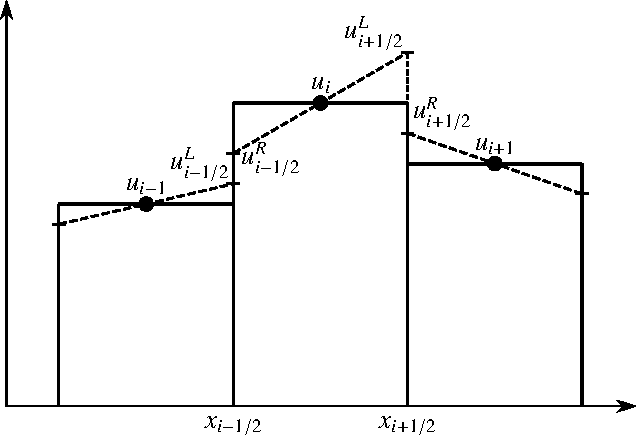
\includegraphics[width=0.5\linewidth]{Pictures/muscl_scheme}
	\caption{Linear reconstruction of the solution at interfaces $x_{i-1/2}$ and $x_{i+1/2}$}
	\label{fig:muscl_scheme}
\end{figure}
Hence, the solution is approximated by a Taylor series expansion around the cell center $x_i$
\begin{equation}
	u(x) = u_i + (x-x_i)\frac{\partial u_i}{\partial x} + \frac{1}{4}(x-x_i)\frac{\partial^2 u_i}{\partial x^2} + \ldots,
	\label{eq:3209423}
\end{equation}
where the derivatives are computed using cell solution differences with respect to neighbouring cells. Note that this reconstruction process can be done using additional terms in Equation~\ref{eq:3209423} to yield higher-order schemes. Hence, on the left and right sides of the interface, the solution can be found by
\begin{align}
	\vec u_{i+1/2}^L &= \vec u_i + \frac{1}{2} \vec \delta_i,\\
	\vec u_{i+1/2}^R &= \vec u_{i+1} - \frac{1}{2} \vec \delta_{i+1},
\end{align}
where the so-called slopes $\delta_i$ can be defined using a blended approach with upwinding parameter $b$
\begin{equation}
	\vec \delta_i = \frac{1}{2}(1+b)\delta \vec u_{i-1/2} + \frac{1}{2}(1-b)\delta \vec u_{i+1/2},
	\label{eq:48742938}
\end{equation}
such that $b=1$ results in an upwind-biased approximation. Considering a linear reconstruction, the solution slopes are given by
\begin{align}
	 \delta \vec u_{i+1/2} = \vec u_{i+1} - \vec u_i, \\
	 \delta \vec u_{i-1/2} = \vec u_{i} - \vec u_{i-1}.
\end{align}
Finally, the common fluxes can be computed using an appropriate Riemann solver of the form
\begin{equation}
	\vec F_{i+1/2} = F(\vec u^L_{i+1/2},\vec  u^R_{i+1/2}).
\end{equation}
\subsection{Second-Order Upwind Scheme for Linear Advection}
For linear advection, a common choice is the upwind Riemann flux given by
\begin{equation}
	F^{upw}(u^L, u^R) = \alpha u^L,
	\label{eq:120398}
\end{equation}
where $\alpha$ is the advection velocity. At the $x_{i+1/2}$ and $x_{i-1/2}$ interfaces, the upwind flux can be found
\begin{align}
	F^{upw}_{i+1/2} = \alpha u^L_{i+1/2} &= \alpha u_i + \frac{\alpha}{2}\delta_i, \label{eq:09809435}\\
	F^{upw}_{i-1/2} = \alpha u^L_{i-1/2} &= \alpha u_{i-1} + \frac{\alpha}{2}\delta_{i-1},
\end{align}
where we choose upwind-biased slopes in Equation~\ref{eq:48742938} with $b=1$ such that
\begin{align}
	\delta_i &= \delta u_{i-1/2} = u_i - u_{i-1}, \\
	\delta_{i-1} &= \delta u_{i-3/2} = u_{i-1} - u_{i-2}.
	\label{eq:98986986}
\end{align}
Hence, using Equations~\ref{eq:09809435}-\ref{eq:98986986}, the common fluxes can be written
\begin{align}
	F_{i+1/2} &= F(u_{i+1/2}) = \alpha u_i + \frac{\alpha}{2}\left(u_i-u_{i-1}\right),\\
	F_{i-1/2} &= F(u_{i-1/2}) = \alpha u_{i-1} + \frac{\alpha}{2}\left(u_{i-1}-u_{i-2}\right),
\end{align}
which yields the following second-order upwind-biased scheme
\begin{eqBox}
	\begin{equation}
		\frac{du_i}{dt} = -\frac{\alpha}{2\Delta x}\left(3u_i - 4 u_{i-1} + u_{i-2}\right).
		\label{eq:34290}
	\end{equation}	
\end{eqBox}
Later in this chapter, we show results of a numerical experiment using this scheme.
\subsection{Total Variation Diminishing}
The total variation (TV) of a scalar conservation law such as the linear advection equation is given by~\cite{hirschNumericalComputationInternal2007a}
\begin{equation}
	TV(u) = \int \left|\frac{\partial u }{\partial x}\right|dx,
\end{equation}
which can be written for the discrete approximation 
\begin{equation}
	TV(u) = \sum_{i=1}^N |u_{i+1}-u_i|,
\end{equation}
where $N$ is the number of finite volume cells. A numerical method is said to be total variation diminishing (TVD) if the solution does not spontaneously concentrate, i.e.
\begin{equation}
	TV(u^t+1)\leq TV(u^t).
\end{equation}
Harten~\cite{harten1997high} proved that TVD schemes are monotonicity-preserving, meaning that in time, maxima does not increase, minima does not decrease, and no new extrema are generated in the solution. It turns out that this property can only be attributed to certain types of schemes. Godunov's theorem states~\cite{godunov1954different}
\begin{theorem}
	Linear numerical schemes for solving partial differential equations (PDE's), having the property of not generating new extrema (monotone scheme), can be at most first-order accurate.
\end{theorem}
Hence, while higher-order schemes are more accurate for smooth solutions, they introduce spurious oscillations in the presence of discontinuities, shocks and large solution gradients and are thus not TVD. Hence, TVD schemes are at most first-order. Different approaches can be used to ensure the TVD property for high-order numerical methods under these circumstances. In the next section, we discuss one of these techniques, known as flux/slope limiters.


\subsection{Limiters}
Introducing limiters to high-order formulations prevents the generation of oscillations in regions where nonsmooth solutions are present. Recall that Godunov's theorem states that only first-order accurate schemes are able to produce solutions without generating new extrema. Hence, limiters are used as a switch mechanism which transforms the high-order numerical scheme into a first-order method in the presence of discontinuities. This is done by evaluating and comparing slopes between neighbouring cells. In this section, we introduce limiters to the MUSCL reconstruction framework in Section~\ref{sec:muscl}.

The MUSCL formulation in Equation~\ref{eq:48742938} can be rewritten for a scalar conservation law using limited slopes 
\begin{align}
	\overline \delta_i = \frac{1}{2}(1+b)\phi^+_{i-1/2}\delta u_{i-1/2} + \frac{1}{2}(1-b)\phi^-_{i+1/2}\delta u_{i+1/2},
	\label{eq:91830192}
\end{align}
where the limiting functions can be defined using ratios of the slopes with neighbouring cells. At interface $x_{i+m}$, the slope limiter is given by
\begin{eqnarray}
	\phi^{\pm}_{i+m} = \phi\left(r^{\pm}_{i+m}\right),\quad r^{\pm}_{i+m} = \frac{\delta u_{i+m\pm 1}}{\delta u_{i+m}}.
\end{eqnarray}
Limiters are designed to treat similarly both upwind and downwind slopes by satisfying the symmetry condition
\begin{equation}
	\frac{\phi(r)}{r} = \phi\left(\frac{1}{r}\right),
\end{equation}
which allows us to simplify Equation~\ref{eq:91830192} to
\begin{eqBox}
	\begin{equation}
		\overline \delta_i = \frac{\phi(r_{i-1/2}^+)}{2} \left[(1+b)\delta u_{i-1/2} + \frac{1}{r_{i-1/2}^+} \delta u_{i+1/2}\right],
	\end{equation}
\end{eqBox}
where
\begin{eqBox}
	\begin{equation}
	r_{i-1/2}^+ = \frac{\delta u_{i+1/2}}{\delta u_{i-1/2}} = \frac{u_{i+1}-u_i}{u_i-u_{i-1}}.
	\end{equation}
\end{eqBox}

For the second-order upwind-biased scheme in Equation~\ref{eq:34290}, we can obtain a scheme with limiting functions using interface fluxes of the form
\begin{align}
	F_{i+1/2} &= F(u_{i+1/2}) = \alpha u_i + \frac{\alpha}{2}\phi(r^+_{i-1/2})\left(u_i-u_{i-1}\right),\\
	F_{i-1/2} &= F(u_{i-1/2}) = \alpha u_{i-1} + \frac{\alpha}{2}\phi(r^+_{i-3/2})\left(u_{i-1}-u_{i-2}\right).
\end{align}
Clearly, in the case $\phi(r) = 0$, the flux reduces to the first-order upwind scheme. This occurs particularly when the limiter detects a change in the slope (negative $r$). Some slope limiting functions are shown in Table~\ref{table:limiters}. In the next section, we show applications of these limiters in the context of linear advection and the Euler equations.
\begin{table}[tb]
	\centering
	\caption{Common forms of limiter functions $\phi(r)$}
	\begin{tabular}{cl}
		\hline
		Name & $\phi(r)$ \\ \hline
		minmod & $\max[0, \min(1, r)]$ \\ 
		van Leer & $\frac{r + |r|}{1 + |r|}$ \\ 
		superbee & $\max[0, \min(2r, 1), \min(r, 2)]$
	\end{tabular}
	\label{table:limiters}
\end{table}

\subsection{Numerical Examples}
\subsubsection{Linear Advection}
Consider the following advection problem
\begin{align}
	\frac{\partial u}{\partial t} + \frac{\partial u}{\partial x} = 0,
\end{align}
on a grid with $x\in[0,2]$ with periodic boundary conditions. The initial conditions at $t=0$ are given by
\begin{align}
	u(x, 0) &= 
	\begin{cases}
		e^{-20(x-0.5)^2} & \text{if } x < 1.2, \\ 
		1 & \text{if } 1.2 < x < 1.5,	 \\
		0 & \text{otherwise}.
	\end{cases}
\end{align}
which consist of a smooth gaussian profile and a step function. Due to the nature of the equation, we expect a translation of the initial condition through the domain without any deformation. At $t=2$, a complete cycle has occurred and it is expected that $u_i^{t=2}\approx u(x_i,0)$. Using the second-order advection scheme with $b=1$ and $N=300$ cells, the solution is shown in Figure~\ref{fig:advection_muscl}. In the smooth region of the domain, the second-order scheme does a good job representing the solution, but we observe that the discontinuities on the right side of the domain contain large oscillations that overshoot and undershoot the exact solution. 

Implementation of the function in Table~\ref{table:limiters} shows the monotonicity of the slope-limited methods. Clearly, the resolution of the shock does not include oscillations, and some limiters introduce more dissipation than others. In all limited cases, observe the crest of the Gauss wave. Due to the slope change of the solution in that region, we have therein introduced additional error.

\begin{figure}[htb]
	\centering
	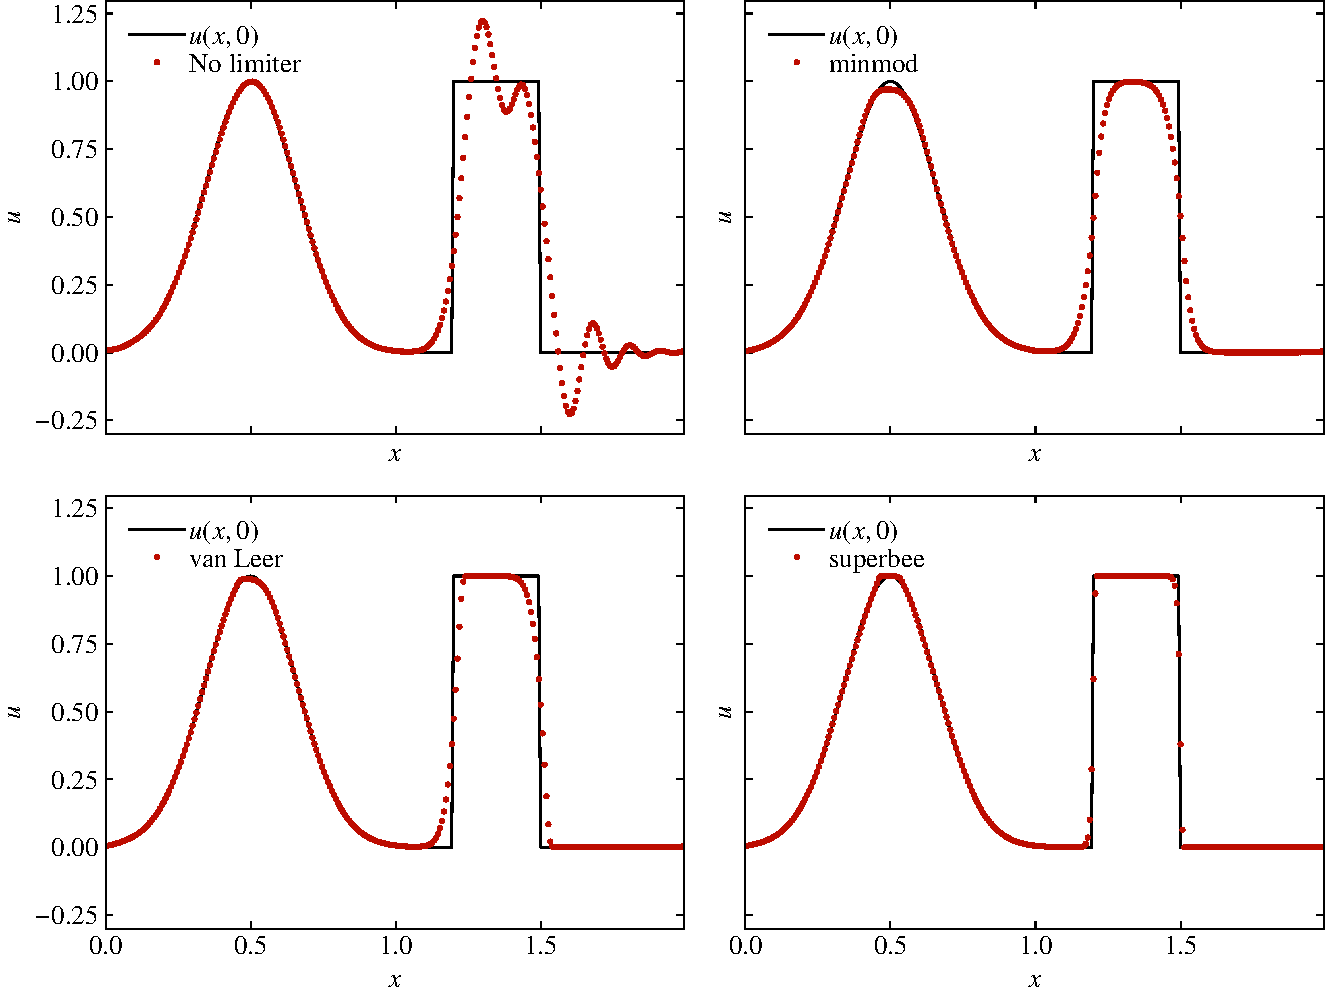
\includegraphics[width=\linewidth]{Pictures/advection_muscl}
	\caption{Second-order upwind-biased advection scheme (upper left) using minmod (upper right), van Leer (lower left) and superbee (lower right) limiters}
	\label{fig:advection_muscl}
\end{figure}

A comparison of the TVD properties of the scheme and other additional assessments can be made using the MUSCL Schemes Jupyter notebook. 
\begin{jupyternote}
	Check out the MUSCL Schemes Jupyter notebook \href{\binderurl}{\underline{here}}. You can also download the files from the Gitlab repository \href{\repourl}{\underline{here}}.
\end{jupyternote}

\subsubsection{Sod's Shock-Tube Problem}
Consider Sod's shock-tube problem with initial conditions
\begin{align}
	\vec u_L = 
	\begin{bmatrix}
		\rho_L \\ v_L \\ p_L 
	\end{bmatrix}
	= 
	\begin{bmatrix}
		1 \\ 0 \\ 1
	\end{bmatrix},
	\quad \text{and} \quad 
	\vec u_R = 
	\begin{bmatrix}
		\rho_R \\ v_R \\ p_R
	\end{bmatrix}
	= 
	\begin{bmatrix}
		\frac{1}{8} \\ 0 \\ \frac{1}{10}
	\end{bmatrix}.
	\label{eq:39248243}
\end{align}
on a domain $x\in[0, 1]$ and $t\in(0,0.2]$. Figure~\ref{fig:euler_muscl} shows a comparison between Godunov's first-order scheme and a linear MUSCL-reconstructed method with different limiters. We note that this problem is unstable for the MUSCL scheme if no limiter function is added. 
The analysis of these results is similar to the advection example and is left as an exercise to the student. The associated Jupyter notebook shows the implementation of these functions for the Euler equations.

\begin{figure}[htb]
	\centering
	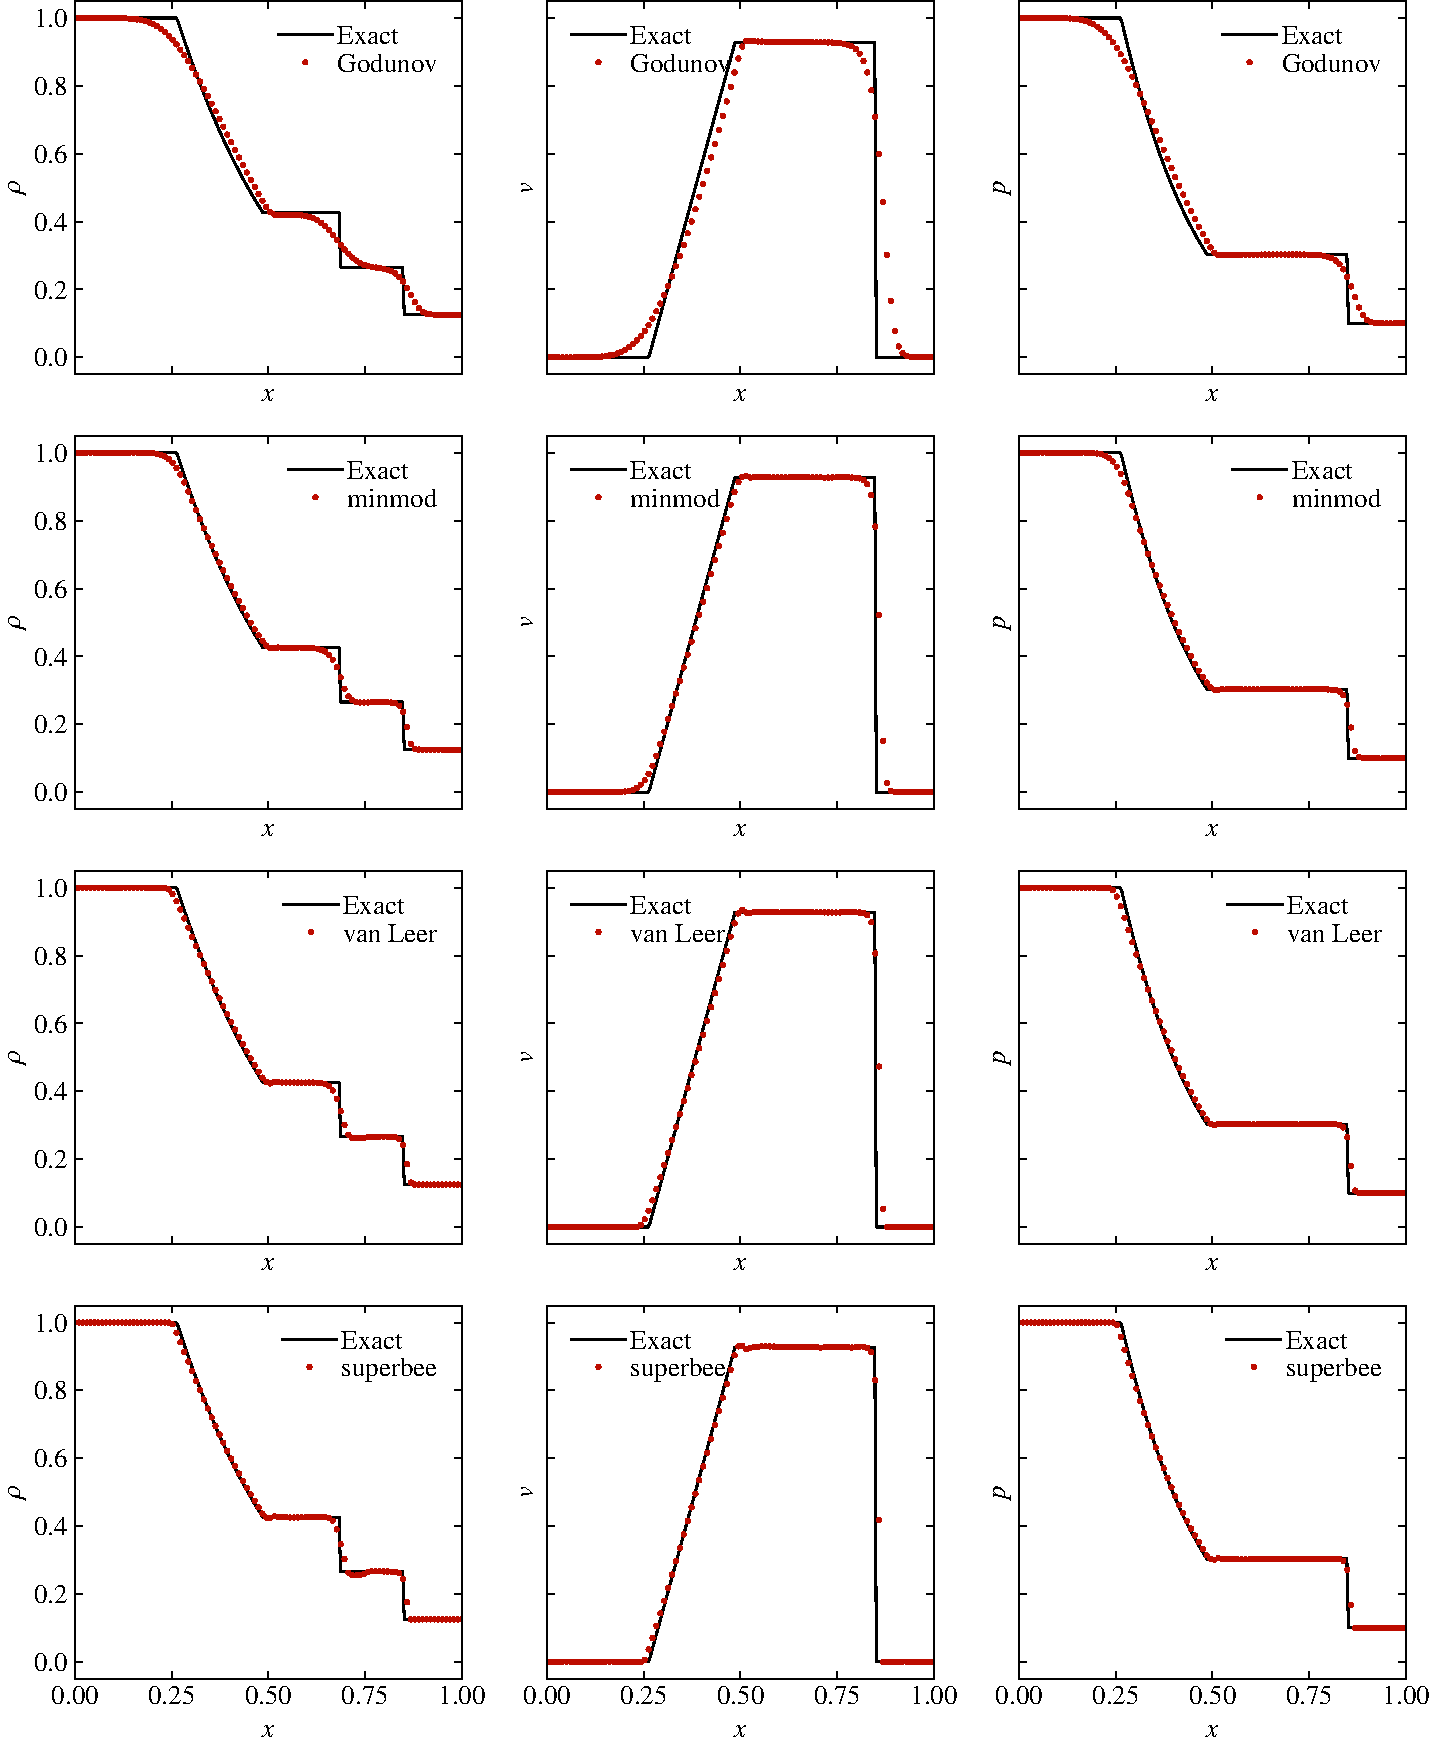
\includegraphics[width=\linewidth]{Pictures/euler_muscl}
	\caption{Results of Sod's shock tube problem at $t=0.2$ with initial conditions in Equation~\ref{eq:39248243}}
	\label{fig:euler_muscl}
\end{figure}
\begin{jupyternote}
	Check out the Sod's Shock-Tube Problem Jupyter notebook \href{\binderurl}{\underline{here}}. You can also download the files from the Gitlab repository \href{\repourl}{\underline{here}}.
\end{jupyternote}

\chapter{Consistency, Stability, Convergence}
Now that we have derived a few different schemes for solving linear advection, Burgers equation, and linear diffusion, we should now ask ourselves whether they will give us accurate predictions, and are there any restrictions on when they can be used. We have already discussed the importance of the order of accuracy, which governs the rate at which the error will converge to zero. Now we will introduce the concepts of consistency, stability, and convergence. If we can prove that our numerical scheme satisfies all three of these properties, we can be confident that it is a promising approach for the Euler or Navier-Stokes equations. In the current section, we will explore these properties in the context of finite difference methods, but the exact same steps can be taken to check whether a finite volume method is suitable or not. Some additional references on these topics include~\cite{hirschNumericalComputationInternal2007a,andersonComputationalFluidMechanics2016}.

\section{Consistency}
A numerical scheme is consistent if it recovers the exact initial partial differential equation as the grid spacing and time step size are reduced. In other words, the truncation error of the scheme must go to zero in the limit $\Delta x \rightarrow 0$ and $\Delta t \rightarrow 0$. This is usually the case, and it is left as an exercise for the reader to check that our previous finite difference schemes for linear advection, Burgers equation, and linear diffusion satisfy this property. 

However, this is not always the case. To demonstrate this, we consider the Dufort-Frankel scheme for linear diffusion
\begin{equation}
u_i^{t+1}  = u_{i}^{t-1} + \frac{2 \beta \Delta t}{\Delta x^2} \left(u_{i-1}^t - u_i^{t+1} - u_i^{t-1} + u_{i+1}^t\right) + \mathcal{O}(\Delta x^2,\Delta t^2,(\Delta t/\Delta x)^2).
\end{equation}
This differs from our example scheme for linear diffusion in that it uses central differences for the time-derivative, and when computing the second-derivative in space, it uses the solution at the current grid point at the previous and current time steps. While this scheme may have some useful properties, we note that it has a peculiar term in the truncation error of $\mathcal{O}((\Delta t/\Delta x)^2)$. This can be obtained from a Taylor series expansion of the second derivative. This is concerning, as for any scheme to be consistent with the original partial differential equation we require the truncation error to go to zero. However, if we use a naive approach and simply refine $\Delta x$ and $\Delta t$ at the same rate, this term will not go to zero, and the scheme will not be consistent. For example, if we reduced both the grid spacing and time step size by a half, this $\mathcal{O}((\Delta t/\Delta x)^2)$ will remain the same. Hence, in order for the Dufort-Frankel scheme to be consistent with our original partial differential equation, we should refine the grid spacing {\it faster} than the time step size. For example, if we reduce $\Delta t$ by a half we should reduce $\Delta x$ by a factor of four. This does not mean the Dufort-Frankel scheme is bad, per-se, but it does mean that care needs to be taken when using it.

\section{Stability}
If we can demonstrate our schemes are consistent, then we know that in the limit $\Delta x \rightarrow 0$ and $\Delta t \rightarrow 0$ we recover the exact partial differential equation. However, this is impossible to achieve in practice as it would require an infinite number of grid points and time steps. When considering stability, we are concerned with whether our numerical scheme will provide {\it physical} solutions when both $\Delta x$ and $\Delta t$ are finite. Let's start by considering what we mean by a physical solution.

In order to advance our solution in time, we start with some initial condition. Then, by inserting this initial condition into our scheme, we approximate the solution at the next timestep $t+\Delta t$. Then, we insert this approximation back into our scheme to approximate the solution at time $t+2\Delta t$, and this process is repeated over and over again until we reach our final desired time. Hence, the way we advance our simulation in time is effectively a feedback loop, with the output of each time step being recycled back through the numerical scheme to get the solution at each consecutive time step. 

As an analogy, we can consider what happens in other simple feedback loops, such as a microphone and speaker. When a performer sings into a microphone, their voice is amplified and played back through the speaker. We expect that this produces a physical replication of their voice, just at a louder volume for the audience. However, if the sound from the speaker is louder than the singer's voice at the microphone, it will get amplified, played through the speaker at a louder volume, and this cycle then repeats. This results in feedback noise, usually a high-pitched ringing that sounds nothing like the original performer, and usually happens when the performer moves to close to the speaker.

Since our numerical scheme is applied as a feedback loop, the exact same kind of thing can happen. If it amplifies our solution each time step, then the solution will continue to grow, eventually leading to non-physical values such as near-infinite density or pressure. This is colloquially referred to as the solution {\it blowing up}. In contrast, if the scheme damps our solution at each time step, it will tend towards physical values, such as the background density or pressure. While this is perhaps not desirable in terms of accuracy, which will be explored later, it is a desirable property in that the solution remains stable and bounded between the initial condition and background state.

Proving stability for non-linear problems, such as Burgers equation, is a relatively daunting task. However, if we restrict ourselves to linear equations, such as linear advection or linear diffusion, then stability can be explored more readily. In order to do this, we introduce {\it Von Neumann Analysis}, also commonly referred to as Fourier Analysis. We first assume that our solution $u(x,t)$ can be represented via a Fourier Series, such that
\begin{equation}
	u(x,t) = \sum_{m} b_m(t) e^{i \kappa_m x},
\end{equation}
where $b_m(t)$ is the Fourier coefficients that vary with time as the solution evolves, $\kappa_m$ is a wavenumber, and in this context $i = \sqrt{-1}$. This is the exact same as a conventional Fourer series, with the exception that the coefficients are a function of time describing the time evolution of the system of equations. Furthermore, we take
\begin{equation}
	\kappa_m = \frac{2 \pi m}{2 L}, \: m=0,1,2,\hdots,M,
\end{equation}
where $M$ is chosen based on the maximum wavenumber that can be represented on the grid based on its Nyquist criteria, and $L$ is the length of the domain. Hence, small values of $\kappa_m$ correspond to large waves, and large values of $\kappa_m$ correspond to very compact waves.

Following this approach, we are taking our solution and decomposing it into a number of different waves via a Fourier series. Now, since we have restricted ourselves to linear systems of equations, we can apply the property of superposition. This means that we can analyze each wave independently as a function of time, and the final solution is simply the superposition of all of these waves. This allows us to analyze the behaviour of our numerical scheme for each wavenumber independently, since they are not coupled. Hence, we can write the solution for one particular wave of the Fourier series as
\begin{equation}
	u_m(x,t) = b_m(t) e^{i \kappa_m x},
\end{equation}
where the complete solution is
\begin{equation}
	u(x,t) = \sum_{m} u_m(x,t).
\end{equation}
We will also assume that the time-dependence of the solution is also wavelike with a prescribed frequency in time such that
\begin{eqBox}
\begin{equation}
	u_m(x,t) = e^{at} e^{i \kappa_m x},
\end{equation}
\end{eqBox}
where $a$ is a complex number, referred to as the numerical frequency, that describes how the solution evolves in time. In order to justify this assumption we can consider the linear advection equation applied to an arbitrary wavenumber $\kappa_m$. We note that this wave will propagate at velocity $\alpha$ from left to right. Now, if we consider some fixed point in space, denoted by $u_1{t}$, we note that the value of the solution in time will alose behave like a sine wave. Hence, at a fixed point in time, the solution has a wavelike structure in space and, at a fixed point in space, the solution has a wavelike structure in time. Hence, the dual wavelike structure taken for $u_m(x,t)$.

With the wavelike structure of the solution described, we can now explore how that wave will change with time. Of primary importance, at least in terms of stability, is to determine whether the wave will be amplified or damped as the solution evolves. Our objective in this section is to determine whether, and under what conditions, numerical schemes satisfy this stability condition. We note that the solution at time $t+\Delta t$ is simply
\begin{equation}
	u_m(x,t+\Delta t) = e^{a(t+\Delta t)} e^{i \kappa_m x},
\end{equation}
which can be re-written as
\begin{equation}
	u_m(x,t+\Delta t) = e^{at}e^{a\Delta t} e^{i \kappa_m x},
\end{equation}
and, in order for the magnitude of the solution to not be amplified at the next time step, we have the stability constraint
\begin{eqBox}
\begin{equation}
	|e^{a\Delta t}| \leq 1,
\end{equation}
\end{eqBox}
which describes a unit circle in the complex plane. Referred to as the amplification factor, we will next determine under what conditions our numerical schemes satisfy this stability constraint.

\subsection{Explicit Linear Advection}
For a methodological approach, we will break von Neumann down into a number of steps.

\subsubsection{Step 1: Choose the Discrete Scheme}
The first step in von Neumann analysis is to determine what scheme we are interested in analyzing. In this case, we will consider our simple first-order scheme for linear advection
\begin{equation}
	\frac{u_i^{t+1} - u_{i}^t}{\Delta t} +  \alpha \frac{u_i^t - u_{i-1}^t}{\Delta x} = 0.
\end{equation}

\subsubsection{Step 2: Apply the Wavelike Solution}
Since we know the prescribed wave-like form of the solution, the grid spacing $\Delta x$, and the time step size $\Delta t$, we can write expressions for the solution for a particular wavenumber $\kappa_m$ at each grid point and time level as
\begin{equation}
	u_{i}^t = e^{at} e^{i \kappa_m x},
\end{equation}
\begin{equation}
	u_{i}^{t+1} = e^{a(t+\Delta t)} e^{i \kappa_m x},
\end{equation}
\begin{equation}
	u_{i-1}^t = e^{at} e^{i \kappa_m (x-\Delta x)}.
\end{equation}
Substituting these into our finite difference approximation yields
\begin{equation}
	\frac{e^{a(t+\Delta t)} e^{i \kappa_m x} - e^{at} e^{i \kappa_m x}}{\Delta t} +  \alpha \frac{e^{at} e^{i \kappa_m x} - e^{at} e^{i \kappa_m (x-\Delta x)}}{\Delta x} = 0.
\end{equation}

\subsubsection{Step 3: Solve for the Amplification Factor}
Noting that all of these terms has a common factor of $e^{at} e^{i \kappa_m x}$ we can simply divide through yielding
\begin{equation}
	\frac{e^{a\Delta t} - 1}{\Delta t} +  \alpha \frac{1 - e^{-i \kappa_m \Delta x}}{\Delta x} = 0.
\end{equation}
Rearranging yields
\begin{equation}
	e^{a\Delta t} = 1 - \sigma + \sigma e^{-i \kappa_m \Delta x},
\end{equation}
where
\begin{equation}
	\sigma = \frac{\alpha \Delta t}{\Delta x},
\end{equation}
is the {\it Courant-Friedrichs-Lewy} (CFL) number. Hence, the amplification factor of our first-order linear advection scheme is 
\begin{eqBox}
\begin{equation}
	|e^{a\Delta t}| = |1 - \sigma + \sigma e^{-i \kappa_m \Delta x}|,
\end{equation}
\end{eqBox}
and our scheme will be stable whenever this is contained within the unit circle in the complex plane. We note that this is a function of two parameters, specifically the wavenumber and the CFL number. Hence, we expect that the amount our solution gets amplified/damped each time step will depend on these two parameters.

\subsubsection{Step 4: Determine the Stability Conditions}
Based on these results, we can conclude that the first-order finite difference scheme for linear advection is stable whenever
\begin{eqBox}
\begin{equation}
	0 \leq \sigma \leq 1.
\end{equation}
\end{eqBox}
That is, it is only stable for CFL numbers less than one. Hence, for a given grid spacing and advection velocity, there is a limit on how large the time step can be. This clearly has implications in terms of computational cost, as the smaller the time step is, the more steps must be taken to reach a desired final solution time. Schemes of this type are referred to as being {\it conditionally stable}.


\begin{figure}[htbp]
	\centering
	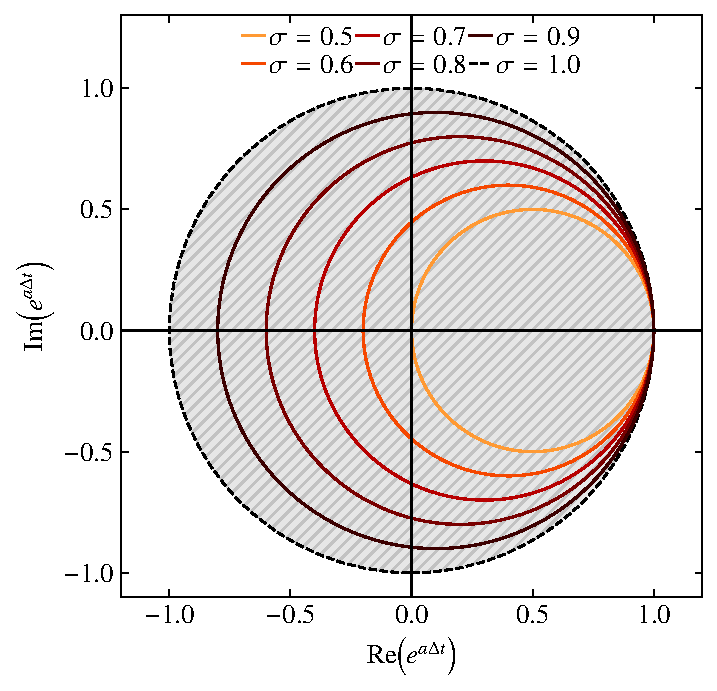
\includegraphics[width=0.6\linewidth]{Pictures/explicit_advection}
	\caption{Stability region for the explicit linear advection scheme.}
	\label{fig:explicit_advection}
\end{figure}

\subsection{Implicit Linear Advection}
In the last section, we saw that our first-order finite difference scheme has a stability limit. In this section, we will explore a slightly different first-order scheme for linear advection.

\subsubsection{Step 1: Choose the Discrete Scheme}
In this case, we use the following finite difference approximation of the linear advection equation
\begin{equation}
	\frac{u_i^{t+1} - u_{i}^t}{\Delta t} +  \alpha \frac{u_i^{t+1} - u_{i-1}^{t+1}}{\Delta x} = 0,
\end{equation}
noting that it is simple the original scheme, but we evaluate the spatial derivative at the next time step rather than the current time step.

\subsubsection{Step 2: Apply the Wavelike Solution}
Our expressions for wavelike solutions at each point are
\begin{equation}
	u_{i}^t = e^{at} e^{i \kappa_m x},
\end{equation}
\begin{equation}
	u_{i}^{t+1} = e^{a(t + \Delta t)} e^{i \kappa_m x},
\end{equation}
\begin{equation}
	u_{i-1}^{t+1} = e^{a(t + \Delta t)} e^{i \kappa_m (x - \Delta x)}.
\end{equation}
Substituting these into our discrete scheme yields
\begin{equation}
	\frac{e^{a(t + \Delta t)} e^{i \kappa_m x} - e^{at} e^{i \kappa_m x}}{\Delta t} +  \alpha \frac{e^{a(t + \Delta t)} e^{i \kappa_m x} - e^{a(t + \Delta t)} e^{i \kappa_m (x - \Delta x)}}{\Delta x} = 0.
\end{equation}

\subsubsection{Step 3: Solve for the Amplification Factor}
Again, we note a common factor of $e^{at} e^{i \kappa_m x}$ in all terms, allowing us to divide through yielding
\begin{equation}
	\frac{e^{a\Delta t} - 1}{\Delta t} +  \alpha \frac{e^{a\Delta t} - e^{a\Delta t} e^{-i \kappa_m \Delta x}}{\Delta x} = 0.
\end{equation}
Rearranging yields
\begin{equation}
	e^{a\Delta t} = \frac{1}{1 + \sigma \left( 1 - e^{-i \kappa_m \Delta x} \right)},
\end{equation}
where $\sigma$ is again the CFL number. Hence, the amplification factor is
\begin{eqBox}
\begin{equation}
	|e^{a\Delta t}| = \left| \frac{1}{1 + \sigma \left( 1 - e^{-i \kappa_m \Delta x} \right)} \right|.
\end{equation}
\end{eqBox}

\subsubsection{Step 4: Determine the Stability Conditions}
Based on these results, we can conclude that this finite difference scheme for the linear advection equation is stable provided
\begin{eqBox}
\begin{equation}
	0 \leq \sigma \leq \infty.
\end{equation}
\end{eqBox}
Hence, we are able to take arbitrarily large time steps and maintain stability using this approach. Schemes of this type are referred to as being {\it unconditionally stable}.

\begin{remark}
Although this scheme is unconditionally stable, making it appealing since it allows for arbitrarily large time-steps, it also becomes more difficult/expensive for each time-step. This will be explored in the forthcoming time stepping section.
\end{remark}

\begin{figure}[htbp]
	\centering
	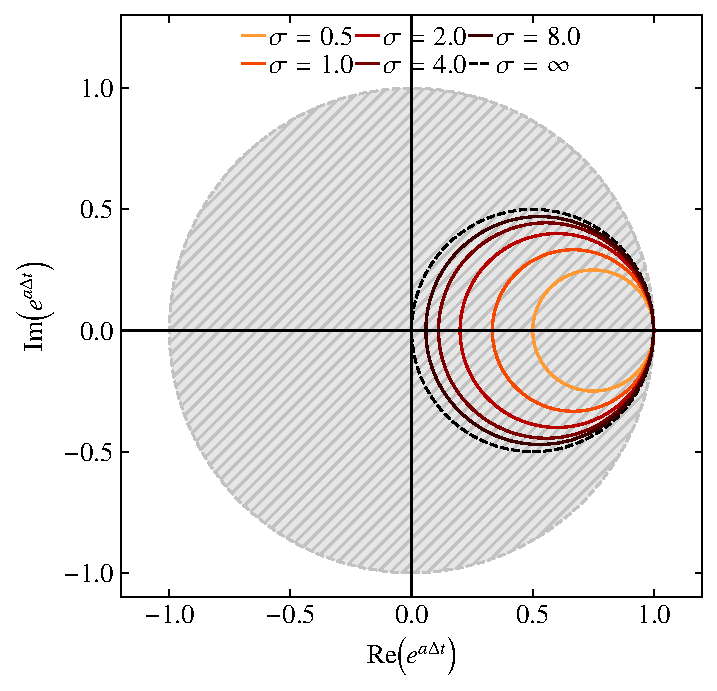
\includegraphics[width=0.6\linewidth]{Pictures/implicit_advection}
	\caption{Stability region for the implicit linear advection scheme.}
	\label{fig:implicit_advection}
\end{figure}

\subsection{Explicit Linear Diffusion}
Similar to the linear advection equation, we can also use von Neumann analysis to analyze the stability of the linear diffusion equation. 

\subsubsection{Step 1: Choose the Discrete Scheme}
We will start with the example scheme we derived in the finite difference section
\begin{equation}
  \frac{u_i^{t+1} - u_{i}^t}{\Delta t} - \beta \frac{u_{i-1}^t - 2u_i^t + u_{i+1}^t}{\Delta x^2} = 0.
\end{equation}

\subsubsection{Step 2: Apply the Wavelike Solution}
Our expressions for wavelike solutions at each point are
\begin{equation}
	u_{i}^t = e^{at} e^{i \kappa_m x},
\end{equation}
\begin{equation}
	u_{i}^{t+1} = e^{a(t + \Delta t)} e^{i \kappa_m x},
\end{equation}
\begin{equation}
	u_{i-1}^{t} = e^{at} e^{i \kappa_m (x - \Delta x)},
\end{equation}
\begin{equation}
	u_{i+1}^{t} = e^{at} e^{i \kappa_m (x + \Delta x)}.
\end{equation}
Substituting these into our discrete scheme yields
\begin{equation}
  \frac{e^{a(t + \Delta t)} e^{i \kappa_m x} - e^{at} e^{i \kappa_m x}}{\Delta t} -  \beta \frac{e^{at} e^{i \kappa_m (x - \Delta x)} - 2e^{at} e^{i \kappa_m x} + e^{at} e^{i \kappa_m (x + \Delta x)}}{\Delta x ^2} = 0.
\end{equation}

\subsubsection{Step 3: Solve for the Amplification Factor}
Again we note a common factor of $e^{at} e^{i \kappa_m x}$ in all terms, allowing us to divide through yielding
\begin{equation}
  \frac{e^{a\Delta t} - 1}{\Delta t} -  \beta \frac{e^{-i \kappa_m \Delta x} - 2 + e^{i \kappa_m \Delta x}}{\Delta x ^2} = 0.
\end{equation}
Rearranging yields
\begin{equation}
	e^{a\Delta t} = 1 + r \left( e^{-i \kappa_m \Delta x} - 2 + e^{i \kappa_m \Delta x} \right), 
\end{equation}
where
\begin{equation}
	r = \frac{\beta \Delta t}{\Delta x^2},
\end{equation}
is similar to the CFL number but for diffusion rather than advection. Finally, the amplification factor is
\begin{eqBox}
\begin{equation}
	|e^{a\Delta t}| = \left| 1 + r \left( e^{-i \kappa_m \Delta x} - 2 + e^{i \kappa_m \Delta x} \right) \right|.
\end{equation}
\end{eqBox}

\subsubsection{Step 4: Determine the Stability Conditions}
Based on this amplification factor, we demonstrate graphically that this scheme will be stable provided
\begin{eqBox}
\begin{equation}
	0 \leq r \leq \frac{1}{2}.
\end{equation}
\end{eqBox}
We note that this scheme is {\it conditionally stable}, similar to the first linear advection scheme we considered. This means if the grid is refined then the time step size must be reduced accordingly to maintain stability. However, we note that the factor of $\Delta x^2$ in $r$ will require the time step size to be reduced with the square of the grid spacing, which can become expensive on finer meshes.

\begin{figure}[htbp]
	\centering
	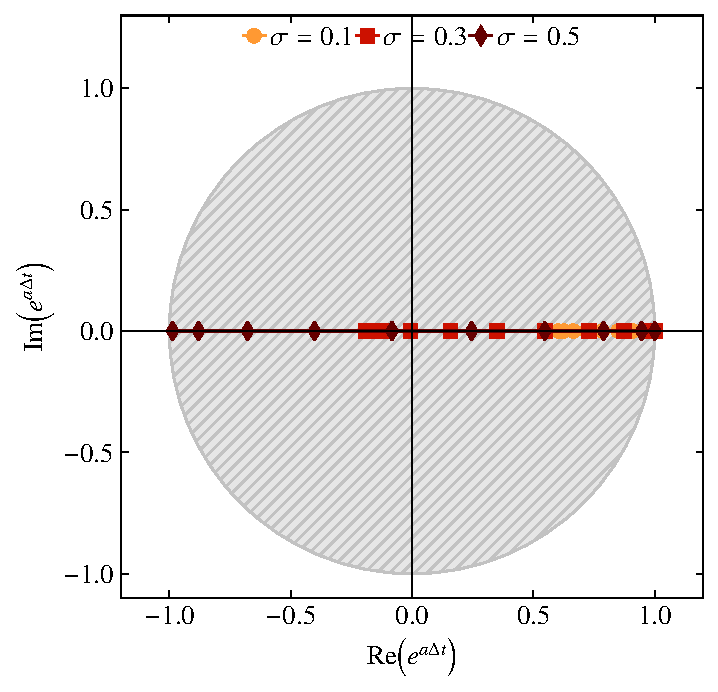
\includegraphics[width=0.6\linewidth]{Pictures/explicit_diffusion}
	\caption{Stability region for the explicit linear diffusion scheme.}
	\label{fig:explicit_diffusion}
\end{figure}

\begin{remark}
The Navier-Stokes equations have both advective and diffusive terms. Hence, the time step is usually limited by the stricter of the stability constraints of the advective and diffusive schemes that are being used.
\end{remark}

\subsection{Implicit Linear Diffusion}
Similar to the modified linear advection scheme, we can also modify our initial linear diffusion scheme by evaluating the spatial operator at the future unknown solution time.

\subsubsection{Step 1: Choose the Discrete Scheme}
This yields the following scheme
\begin{equation}
  \frac{u_i^{t+1} - u_{i}^t}{\Delta t} - \beta \frac{u_{i-1}^{t+1} - 2u_i^{t+1} + u_{i+1}^{t+1}}{\Delta x^2} = 0.
\end{equation}

\subsubsection{Step 2: Apply the Wavelike Solution}
Our expressions for wavelike solutions at each point are
\begin{equation}
	u_{i}^t = e^{at} e^{i \kappa_m x},
\end{equation}
\begin{equation}
	u_{i}^{t+1} = e^{a(t + \Delta t)} e^{i \kappa_m x},
\end{equation}
\begin{equation}
	u_{i-1}^{t+1} = e^{a(t + \Delta t)} e^{i \kappa_m (x - \Delta x)},
\end{equation}
\begin{equation}
	u_{i+1}^{t+1} = e^{a(t + \Delta t)} e^{i \kappa_m (x + \Delta x)}.
\end{equation}
Substituting these into our discrete scheme yields
\begin{equation}
  \frac{e^{a(t + \Delta t)} e^{i \kappa_m x} - e^{at} e^{i \kappa_m x}}{\Delta t} - \beta \frac{e^{a(t + \Delta t)} e^{i \kappa_m (x - \Delta x)} - 2e^{a(t + \Delta t)} e^{i \kappa_m x} + e^{a(t + \Delta t)} e^{i \kappa_m (x + \Delta x)}}{\Delta x^2} = 0.
\end{equation}

\subsubsection{Step 3: Solve for the Amplification Factor}
Again we note a common factor of $e^{at} e^{i \kappa_m x}$ in all terms, allowing us to divide through yielding
\begin{equation}
  \frac{e^{a\Delta t} - 1}{\Delta t} - \beta \frac{e^{a\Delta t} e^{-i \kappa_m \Delta x} - 2e^{a\Delta t} + e^{a\Delta t} e^{i \kappa_m \Delta x}}{\Delta x^2} = 0.
\end{equation}
Rearranging yields
\begin{equation}
e^{a\Delta t}	= \frac{1}{\left[ 1 - r \left(e^{-i \kappa_m \Delta x} - 2 + e^{i \kappa_m \Delta x} \right)  \right]},
\end{equation}
where $r$ is the same as the original linear diffusion scheme. Finally, the amplification factor is
\begin{eqBox}
\begin{equation}
	|e^{a\Delta t}|	= \left| \frac{1}{\left[ 1 - r \left(e^{-i \kappa_m \Delta x} - 2 + e^{i \kappa_m \Delta x} \right)  \right]} \right|.
\end{equation}
\end{eqBox}

\subsubsection{Step 4: Determine the Stability Conditions}
Based on the form of the amplification factor, we can conclude that this scheme will be stable for
\begin{eqBox}
\begin{equation}
	0 \leq r \leq \infty.
\end{equation}
\end{eqBox}
Hence, this linear diffusion scheme is {\it unconditionally stable}.
\begin{figure}[htbp]
	\centering
	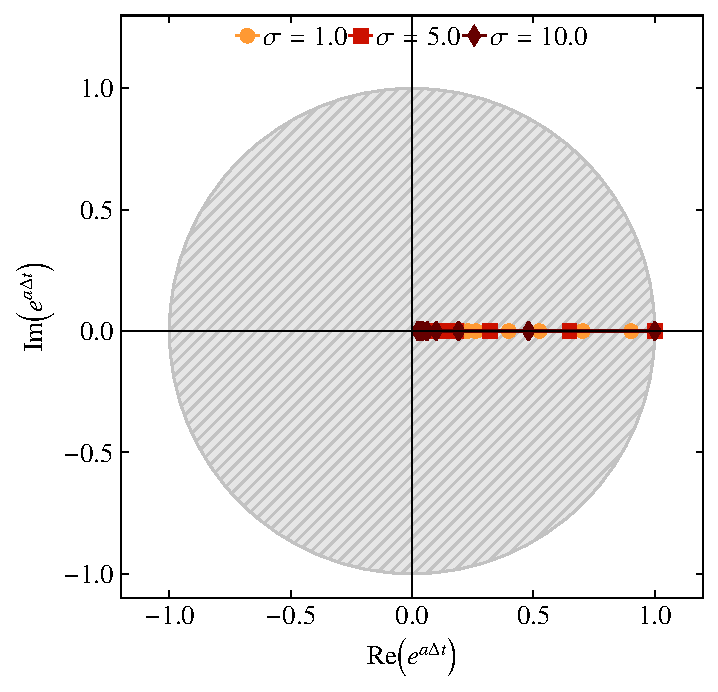
\includegraphics[width=0.6\linewidth]{Pictures/implicit_diffusion}
	\caption{Stability region for the implicit linear diffusion scheme.}
	\label{fig:implicit_diffusion}
\end{figure}

\section{Convergence}
If a scheme is consistent, recovering the exact partial differential equation in the limit $\Delta x \rightarrow 0$ and $\Delta t \rightarrow 0$, and stable, in that the approximate solution does not grow unbounded with time, then Lax's equivalence theorem can be applied. In summary, the theorem states that when given a properly-posed initial value problem, and a numerical scheme that is consistent, stability is the necessary and sufficient condition for convergence. In other words, if we can show that our numerical schemes are consistent and stable, then we can be sure that it will {\it converge} to the true solution of the partial differential equation in the limit $\Delta x \rightarrow 0$ and $\Delta t \rightarrow 0$.

\chapter{Spectral Properties}\label{ch:spectralproperties}
In CFD, the numerical error introduced by a scheme is typically classified into two general types, dissipation error and dispersion error. In this section, we will discuss how to quantify these two types of error, and how they effect different types of solutions.

\begin{figure}[htbp]
	\centering
	\begin{subfigure}[b]{0.49\linewidth}
		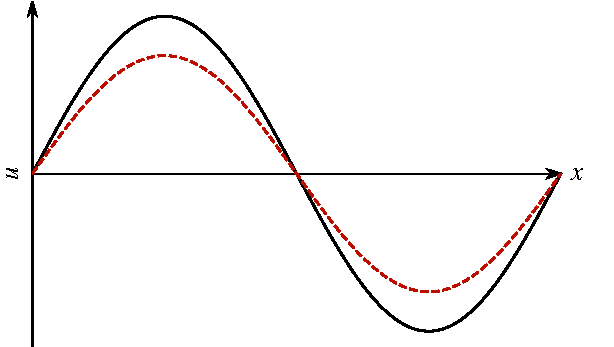
\includegraphics[width=\linewidth]{Pictures/dissipation_diagram}
		\caption{Dissipation}
	\end{subfigure}
	\begin{subfigure}[b]{0.49\linewidth}
		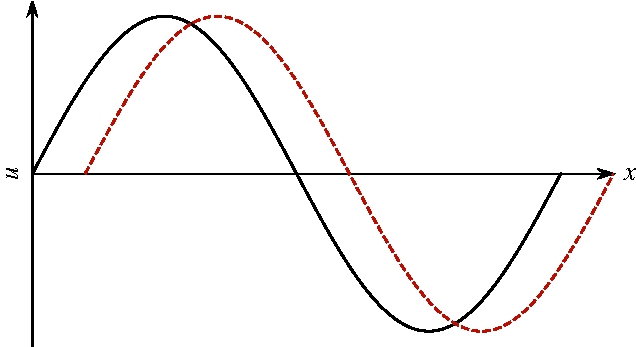
\includegraphics[width=\linewidth]{Pictures/dispersion_diagram}
		\caption{Dispersion}
	\end{subfigure}
	\caption{Types of numerical error}
	\label{fig:numerical_error}
\end{figure}



\section{Dissipation Error}
We have already discussed dissipation error in the context of stability, stating that in order for a scheme to be stable, it must be dissipative or neutrally dissipative. That is, the amplitude of the solution must remain the same or be reduced after each time step. We have shown this via von Neumann analysis to be the amplification factor $|e^{a\Delta t}|$, which was a function of the scheme we are using, and the wavenumber in space $\kappa_m$. While a scheme being dissipative is inherently linked with stability, it also introduces number error. For example, for the linear advection equation, we know that the exact solution should have no dissipation, it should be simply the advection of the initial condition with the prescribed advection velocity. However, with our initial finite difference scheme, we found that this was not the case, and the amplitude of the waves is decreased as time goes on.

It turns out that all the information we need to understand the dissipation error of the linear advection equation is encoded in the amplification factors we found in the von Neumann analysis section, $|e^{a\Delta t}|$. For example, for the finite difference scheme
\begin{equation}
	\frac{u_i^{t+1} - u_{i}^t}{\Delta t} +  \alpha \frac{u_i^t - u_{i-1}^t}{\Delta x} = 0.
\end{equation}
we found that the amplification factor was 
\begin{equation}
	|e^{a\Delta t}| = |1 - \sigma + \sigma e^{-i \kappa_m \Delta x}|.
\end{equation} 
Recall that, for a given wavenumber $\kappa_m$ and CFL number $\sigma$, this told us how much the solution will be damped over a time step. Hence, we can plot this for a range of permissible wavenumbers in the range $\kappa_m \Delta x \in [0,\pi]$ and CFL numbers within the stability limit $\sigma \in [0,1]$. A plot of this is shown in Figure \ref{fig:dissipation_advection_explicit}. We can observe a few interesting features that define the dissipation error of this particular scheme. First, we note that when the wave size is large relative to the grid spacing, the wave is well resolved regardless of the CFL number. However, as we move to larger wavenumbers, there is significant numerical dissipation. Also, the amount of numerical in this region dissipation depends on the CFL number, with larger CFL numbers corresponding to less dissipation. Finally, when the CFL number approaches unity, the numerical dissipation approaches zero for all wavenumbers. Hence, when this CFL number is used, we recover the exact dissipation relation for linear advection, that the waves do not get damped. The dissipation error of this scheme becomes particularly important in the context of turbulent flows. In this case, large scale structures in the turbulent flow have small wavenumbers relative to the grid spacing. This means that our large scale features will be simulated with relative accuracy. However, small scale turbulent structures that are of a size proportional to the grid spacing have high relative wavenumbers. This means that these fine-scale structures will be heavily dissipated by this first-order scheme.
\begin{figure}[htbp]
	\centering
	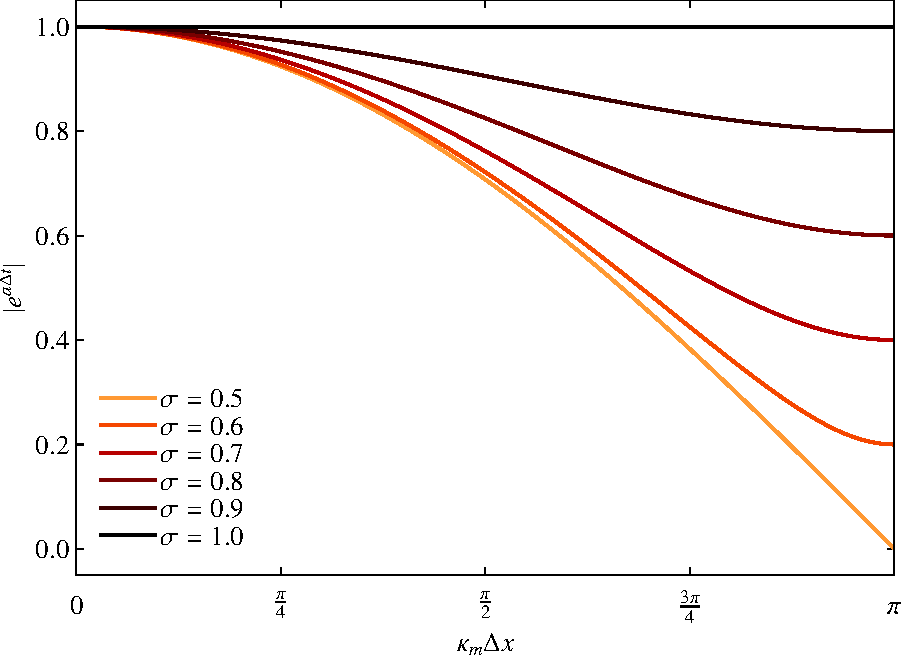
\includegraphics[width=0.6\linewidth]{Pictures/dissipation_adv_explct}
	\caption{Amplification factor vs wavenumber for the explicit advection scheme}
	\label{fig:dissipation_advection_explicit}
\end{figure}
Let's look at a second example, our implicit finite difference scheme
\begin{equation}
	\frac{u_i^{t+1} - u_{i}^t}{\Delta t} +  \alpha \frac{u_i^{t+1} - u_{i-1}^{t+1}}{\Delta x} = 0,
\end{equation}
that had the amplification factor
\begin{equation}
	|e^{a\Delta t}| = \left| \frac{1}{1 + \sigma \left( 1 - e^{-i \kappa_m \Delta x} \right)} \right|.
\end{equation}
We can generate the exact same type of plot for permissible wave numbers $\kappa_m \Delta x \in [0,\pi]$ and, since this scheme is unconditionally stable, we will look at a few CFL numbers in the range $\sigma \in [0,10]$, as shown in Figure \ref{fig:dissipation_advection_implicit}. We note for this scheme, similar to the explicit scheme, that when the wave size is large relative to the grid spacing, it is well resolved regardless of the CFL number. However, there is again a strong dependence of the numerical dissipation on the CFL number for high wavenumbers. As the wavenumber gets larger or as the CFL number gets larger, the amount of numerical dissipation increases rapidly. Hence, while this scheme was found to be unconditionally stable, using large CFL numbers introduces significant numerical dissipation to all but the largest structures in the flow. Hence, this scheme is typically only used for solving steady-state problems that are not a function of time.
\begin{figure}[htbp]
	\centering
	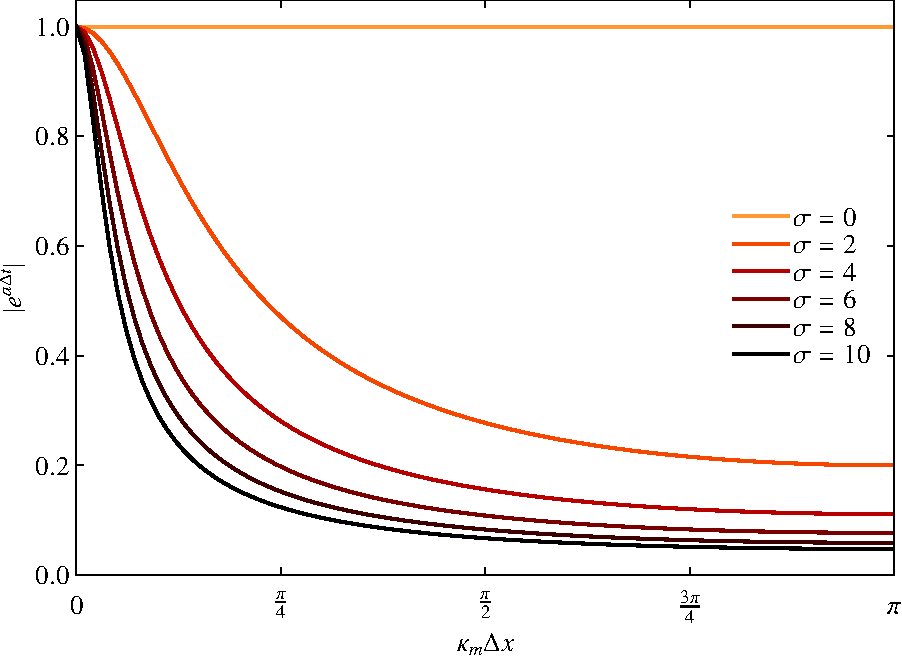
\includegraphics[width=0.6\linewidth]{Pictures/dissipation_adv_implct}
	\caption{Amplification factor vs wavenumber for the implicit advection scheme}
	\label{fig:dissipation_advection_implicit}
\end{figure}
\begin{jupyternote}
	Check out the Von Neumann Jupyter notebook \href{\binderurl}{\underline{here}}. You can also download the files from the Gitlab repository \href{\repourl}{\underline{here}}.
\end{jupyternote}
\section{Dispersion Error}
From the linear advection equation, we know that the solution should translate at an exact wave speed $\alpha$. However, our numerical schemes will often introduce another error whereby the numerical wave does not move at the correct velocity. As a result, we often observe that the numerical solution is out of phase with the exact solution, which is referred to as dispersion error. Similar to the dissipation error, dispersion error can also be found from our results from von Neumann analysis. Recall that our assumed form of the solution for any isolated wave component of the full solution was
\begin{equation}
	u_m(x,t) = e^{at} e^{i \kappa_m x},
\end{equation}
and recall the expression for the linear advection equation was
\begin{equation}
	\frac{\partial u}{\partial t} +  \alpha \frac{\partial u}{\partial x} = 0.
\end{equation}
If we substitute our wavelike solution we get
\begin{equation}
	ae^{at} e^{i \kappa_m x} + i \alpha \kappa_m e^{at} e^{i \kappa_m x} = 0.
\end{equation}
We note that this will be solved exactly when
\begin{eqBox}
\begin{equation}
	a = -i \alpha \kappa_m.
\end{equation}
\end{eqBox}
which is called the exact dispersion relation. This tells us that the exact frequency in time, which is described by $a$, is proportional to the wave speed and the wavenumber. Intuitively this makes sense as the faster a wave moves, the more the solution at a point should move up and down, and the higher the wavenumber, the more quickly the wave will move up and down in time as well. However, our numerical scheme will usually not return a value of $a$ that matches this dispersion relation exactly. Hence, for a given wavenumber, we will get back a frequency that has some error, implying that the wave is moving at the wrong speed, which is referred to as dispersion error. Over a finite amount of time $\Delta t$, based on the exact dispersion relation, we would expect the wave to move a distance
\begin{equation}
	a \Delta t = -i \alpha \kappa_m \Delta t.
\end{equation}

We note that we can also get to our numerical frequency from von Neumann analysis. For example, for the finite difference scheme
\begin{equation}
	\frac{u_i^{t+1} - u_{i}^t}{\Delta t} +  \alpha \frac{u_i^t - u_{i-1}^t}{\Delta x} = 0,
\end{equation}
we found
\begin{equation}
	e^{a\Delta t} = 1 - \sigma + \sigma e^{-i \kappa_m \Delta x},
\end{equation} 
which was the last step before getting the amplification factor. We can start by splitting the exponential term up into its real and imaginary parts
\begin{equation}
	e^{\Re{(a)}\Delta t} e^{\Im{(a)}\Delta t} = 1 - \sigma + \sigma e^{-i \kappa_m \Delta x}.
\end{equation} 
We first note that the real part of this $e^{\Re{(a)}\Delta t}$ is responsible for the amplification/dissipation of the solution, and is what is extracted in the dissipation section. In contrast, the imaginary part $e^{\Im{(a)}\Delta t}$ is responsible for a change in phase of the wave, which moves it in space. We can extract this imaginary term that is responsible for the phase change from
\begin{equation}
	a\Delta t = \ln \left(1 - \sigma + \sigma e^{-i \kappa_m \Delta x} \right),
\end{equation} 
and then extract the imaginary components
\begin{equation}
	\Im(a\Delta t) = \Im{ \left[ \ln \left(1 - \sigma + \sigma e^{-i \kappa_m \Delta x} \right) \right]}.
\end{equation}
In the ideal case, this should be identical to the exact dispersion relation, but in practical applications, it is typically either slower or faster, resulting in some phase error from the wave moving at an approximate speed. We can extract the relative speed from
\begin{equation}
	\frac{\Im(a\Delta t)}{-i \alpha \kappa_m \Delta t} = \frac{\Im{ \left[ \ln \left(1 - \sigma + \sigma e^{-i \kappa_m \Delta x} \right) \right]}}{-i \alpha \kappa_m \Delta t},
\end{equation}
which tells us the speed of the numerical wave relative to the exact wave speed. When this value is less than 1 the wave moves too slowly, and when this value is greater than 1 the wave moves to fast.
\begin{figure}[htbp]
	\centering
	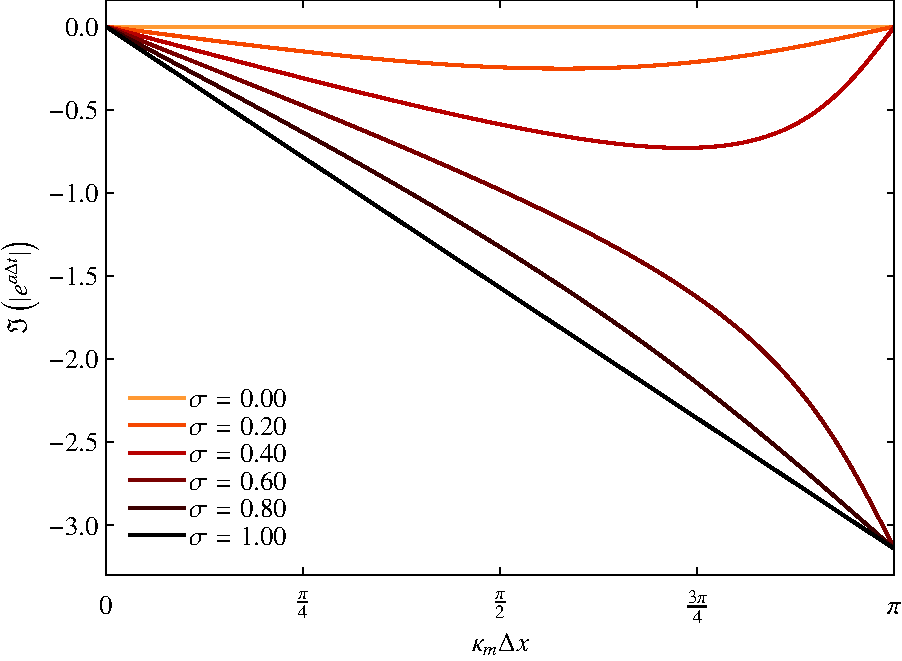
\includegraphics[width=0.6\linewidth]{Pictures/dispersion_adv_explct}
	\caption{Dispersion curve for the implicit advection scheme}
	\label{fig:dissipation_advection_implicit}
\end{figure}
\begin{jupyternote}
	Check out the Von Neumann Jupyter notebook \href{\binderurl}{\underline{here}}. You can also download the files from the Gitlab repository \href{\repourl}{\underline{here}}.
\end{jupyternote}
\chapter{Modified Equation Analysis}
In the previous sections, we have demonstrated that our numerical schemes only approximate the exact PDE we are trying to solve. Furthermore, via von Neumann analysis, we can quantify the type of error we will observe as either dissipation or dispersion. Modified equation analysis is another powerful technique that allows us to better understand how and why a particular numerical scheme behaves the way it does. Using modified equation analysis, we can show that, while our numerical scheme does not exactly satisfy the PDE we are trying to solve, it does provide an exact solution to a similar PDE. By determining what this similar PDE is, we can gain further insight into the behaviour of our scheme. In this section, we will demonstrate by example how to perform modified equation analysis in the context of linear advection.

\section{Linear Advection}
Here, we will derive the modified equation for our first order linear advection scheme
\begin{equation}
	\frac{u_i^{t+1} - u_{i}^t}{\Delta t} +  \alpha \frac{u_i^{t} - u_{i-1}^{t}}{\Delta x} = 0.
\end{equation}
In order to derive the modified equation, we will start by re-stating our Taylor-Series expansions for the solution at each grid point and time level, dropping the evaluated at notation for compactness and expanding up to the second-order terms, as
\begin{equation}
	u_{i-1}^t = u_i^t - \Delta x \frac{\partial u}{\partial x} + \frac{\Delta x^2}{2} \frac{\partial^2 u}{\partial x^2} + \mathcal{O}(\Delta x^3),
\end{equation}
and using a similar Taylor-Series in time
\begin{equation}
	u_{i}^{t+1} = u_i^t - \Delta t \frac{\partial u}{\partial t} + \frac{\Delta t^2}{2} \frac{\partial^2 u}{\partial t^2} + \mathcal{O}(\Delta t^3).
\end{equation}
We will now insert these expansions into our numerical scheme for their respective terms
\begin{equation}
	\frac{u_i^t - \Delta t \frac{\partial u}{\partial t} + \frac{\Delta t^2}{2} \frac{\partial^2 u}{\partial t^2} + \mathcal{O}(\Delta t^3) - u_{i}^t}{\Delta t} +  \alpha \frac{u_i^{t} - u_i^t - \Delta x \frac{\partial u}{\partial x} + \frac{\Delta x^2}{2} \frac{\partial^2 u}{\partial x^2} + \mathcal{O}(\Delta x^3)}{\Delta x} = 0.
\end{equation}
Simplifying this expression down a bit yields
\begin{equation}
	- \frac{\partial u}{\partial t} + \frac{\Delta t}{2} \frac{\partial^2 u}{\partial t^2} + \mathcal{O}(\Delta t^2) +  \alpha \left[ - \frac{\partial u}{\partial x} + \frac{\Delta x}{2} \frac{\partial^2 u}{\partial x^2} + \mathcal{O}(\Delta x^2) \right] = 0,
\end{equation}
which can then be rearranged to
\begin{equation}
	\label{eqn:38fg93la}
	\frac{\partial u}{\partial t} + \alpha \frac{\partial u}{\partial x} = -\frac{\Delta t}{2} \frac{\partial^2 u}{\partial t^2} + \alpha \frac{\Delta x}{2} \frac{\partial^2 u}{\partial x^2} + \mathcal{O}(\Delta x^2,\Delta t^2).
\end{equation}
We can recognize the right-hand side of this equation as the truncation error of our scheme and we note that in the limit as $\Delta t$ and $\Delta x$ go to zero this will converge to the exact PDE. Furthermore, since the behaviour of the temporal derivative on the left-hand side is somewhat unclear, we will convert it to a spatial derivative. Starting by differentiating the above expression in time, we get
\begin{equation}
	\label{eqn:pelfhv72}
	\frac{\partial^2 u}{\partial t^2} + \alpha \frac{\partial^2 u}{\partial x \partial t} = -\frac{\Delta t}{2} \frac{\partial^3 u}{\partial t^3} + \alpha \frac{\Delta x}{2} \frac{\partial^3 u}{\partial x^2 \partial t} + \mathcal{O}(\Delta x^2,\Delta t^2),
\end{equation}
and in space, we get
\begin{equation}
	\label{eqn:dhwis937}
	\frac{\partial^2 u}{\partial t \partial x} + \alpha \frac{\partial^2 u}{\partial x^2} = -\frac{\Delta t}{2} \frac{\partial^3 u}{\partial t^2 \partial x} + \alpha \frac{\Delta x}{2} \frac{\partial^3 u}{\partial x^3} + \mathcal{O}(\Delta x^2,\Delta t^2).
\end{equation}
Rearranging and substituting Equation \ref{eqn:dhwis937} into Equation \ref{eqn:pelfhv72} yields
\begin{equation}
	\frac{\partial^2 u}{\partial t^2} = \alpha^2 \frac{\partial^2 u}{\partial x^2} + \mathcal{O}(\Delta x,\Delta t).
\end{equation}
Hence, if we go back to Equation \ref{eqn:38fg93la} we can replace our second derivative in time with a second derivative in space, yielding
\begin{equation}
	\label{eqn:38fg93la}
	\frac{\partial u}{\partial t} + \alpha \frac{\partial u}{\partial x} = -\frac{\Delta t}{2} \alpha^2 \frac{\partial^2 u}{\partial x^2} + \alpha \frac{\Delta x}{2} \frac{\partial^2 u}{\partial x^2} + \mathcal{O}(\Delta x^2,\Delta t^2,\Delta x\Delta t^2,\Delta t^3).
\end{equation}
Then, using the definition of the CFL number previously defined as $\sigma = \alpha \Delta t / \Delta x$
\begin{equation}
	\frac{\partial u}{\partial t} + \alpha \frac{\partial u}{\partial x} = \frac{\alpha \Delta x}{2}(1-\sigma) \frac{\partial^2 u}{\partial x^2} + \mathcal{O}(\Delta x^2,\Delta t^2,\Delta x\Delta t^2,\Delta t^3),
\end{equation}
and rearranging finally yields
\begin{eqBox}
\begin{equation}
	\label{eqn:shrj986g}
	\frac{\partial u}{\partial t} + \alpha \frac{\partial u}{\partial x} - \frac{\alpha \Delta x}{2}(1-\sigma) \frac{\partial^2 u}{\partial x^2} = \mathcal{O}(\Delta x^2,\Delta t^2,\Delta x\Delta t^2,\Delta t^3).
\end{equation}
\end{eqBox}

If we look at the form of the Equation \ref{eqn:shrj986g}, we see that when $\Delta x$ and $\Delta t$ are small the right-hand side reduces to zero, and we are left with a general {\it advection-diffusion} equation. Hence, we have shown that our finite difference scheme is actually the exact solution to an advection-diffusion problem, rather than the linear advection equation we initially intended to solve. Furthermore, we note that the diffusion operator will only be valid for $0 \leq \sigma \leq 1$, after which point the sign of the term will change and it will become a non-physical {\it anti-diffusive} operator. This switch from a physical to non-physical PDE coincides with the stability limits we had originally derived for this scheme using von Neumann analysis. Also, as we would expect, our solutions using this method also behave exactly like an advection-diffusion equation since the solution also move, but simultaneously dissipates. Also, for the value $\sigma=1$, this diffusion operator disappears, which is also consistent with our observations and predictions based on von Neumann analysis, which showed that the amplification factor $| e^{a \Delta t} | = 1$ for this case.

\section{General Observations}
It is important to note that the procedure followed here for the first order linear advection scheme can be repeated for any finite difference scheme of your choice. Starting with your numerical scheme, you can replace each term with its Taylor Series expansion and rearrange this to try to get the PDE of interest on the left-hand side and truncation error on the right-hand side. The leading order terms will tell you the nature of the dominant error in the scheme. If the dominant error has an even-order derivative, such as the scheme above, then one would expect that the scheme is {\it dominantly dissipative}. In contrast, if the dominant error has an odd-order derivative, then one would expect that the scheme is {\it dominantly dispersive}. Hence, similar to von Neumann analysis, modified equation analysis is a powerful tool to aid in understanding the general behaviour of a numerical scheme, to elucidate its dissipative and dispersive error properties, and to identify its stability limits.

\chapter{Time-Stepping}
\label{ch:timestepping}
In the previous sections, we have always approximated the time derivative using first-order finite differences, assuming
\begin{equation}
	\frac{\partial u}{\partial t} = \frac{u_i^{t+1} - u_{i}^t}{\Delta t} + \mathcal{O}(\Delta t).
\end{equation}
In the von Neumann analysis section, we demonstrated that two linear advection schemes and two linear diffusion schemes are either conditionally or unconditionally stable using this approach. However, if we try to use this finite difference approach to get higher-order accurate schemes in time, such as a central in time approach
\begin{equation}
	\frac{\partial u}{\partial t} = \frac{u_i^{t+1} - u_{i}^{t-1}}{2 \Delta t} + \mathcal{O}(\Delta t^2),
\end{equation}
we find it is almost always {\it unstable}. Hence, getting higher than first-order accurate solutions in time requires something other than finite differences. Furthermore, for both of the unconditionally stable schemes in the von Neumann section, we have not yet discussed how to actually advance them in time, and how to get higher-order accuracy in time, while maintaining this unconditional stability. Hence, in this section, we will discuss more appropriate discretizations for the time derivative.

\section{Explicit}
Our previous approach for discretizing the time derivative is called a {\it multi-step} scheme since we are using information from multiple time steps to try to estimate the solution at the next time-step. In this section we will introduce {\it multi-stage} time stepping, specifically the well-known classical Runge-Kutta methods. Rather than use the value of the solution at previous time steps, Runge-Kutta methods compute the solution at intermediate stages between time level $t$ and $t+1$. Then, these intermediate solutions are cleverly combined to achieve a more stable and potentially higher-order accurate solution in time. In all of these cases, we will re-arrange our system into a general form
\begin{equation}
	\frac{\partial u}{\partial t} = R(u),
\end{equation}
where $R(u)$ is typically referred to as the {\it residual} or the {\it right-hand side}. Note that the term residual is used in several different contexts in CFD.

\subsection{Forward Euler}
The forward Euler, or explicit Euler, scheme uses just one stage to predict the solution at the next time step. In fact, it is equivalent to our previous finite difference approach. In this scheme we get
\begin{equation}
	u^{t+1} = u^t + \Delta t R(u).
\end{equation}
Graphically, this can be interpreted as using the current derivative of the solution in time at time $t$, and simply extrapolating based on this derivative to the time $t+1$. This approach is $\mathcal{O}(\Delta t)$ in time.
\begin{figure}[htbp]
	\centering
	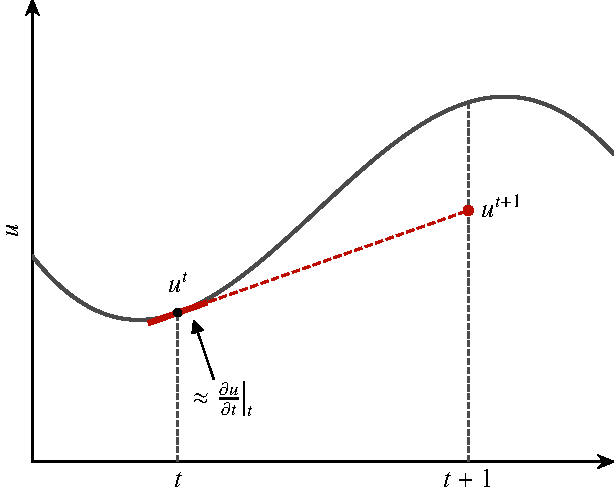
\includegraphics[width=0.6\linewidth]{Pictures/explicit_euler}
	\caption{Explicit Euler}
	\label{fig:explicit_euler_method}
\end{figure}
\subsection{Heun's Method}
Heun's method is a fairly simple but clever improvement on the explicit Euler scheme. We start by using the explicit Euler method to build an approximation of the solution at $t+1$
\begin{equation}
	\tilde{u} = u^t + \Delta t R(u),
\end{equation}
where $\tilde{u}$ is an initial guess for the solution. Then, we use an average of the following right-hand sides to compute the solution at the next time step
\begin{equation}
	\tilde{u}^{t+1} = u^t + \Delta t \left[\frac{R(u) + R(\tilde{u})}{2} \right].
\end{equation}
This approach is called a two-stage scheme, since we had to compute our solution at one intermediate stage before the final solution is obtained. This requires us to evaluate two right-hand sides, one for each stage, so is approximately twice as expensive as the explicit Euler method. However, it can be shown that it achieves $\mathcal{O}(\Delta t^2)$ in time. Hence, when the time step is small, it is significantly more accurate.
\begin{figure}[htbp]
	\centering
	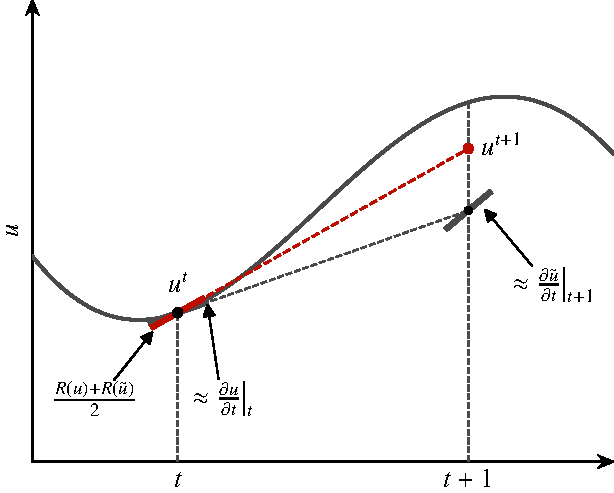
\includegraphics[width=0.6\linewidth]{Pictures/heuns_method}
	\caption{Heun's method}
	\label{fig:heuns_method}
\end{figure}

\subsection{Midpoint Method}
The midpoint method is very similar to Heun's method. However, we start by computing the solution at an intermediate stage halfway between the current and next time steps, using an explicit Euler approach
\begin{equation}
	\tilde{u} = u^t + \frac{\Delta t}{2} R(u).
\end{equation}
Since we have divided $\Delta t$ by two, we are now halfway between the current and next time steps, hence why it is called the midpoint method. Now, we compute the solution at the next time step by evaluating the residual at this midpoint location
\begin{equation}
	u^{t+1} = u^t + \Delta t R(\tilde{u}).
\end{equation}
Similar to Heun's method, this is also a two stage scheme and has a temporal error of $\mathcal{O}(\Delta t^2)$.
\begin{figure}[htbp]
	\centering
	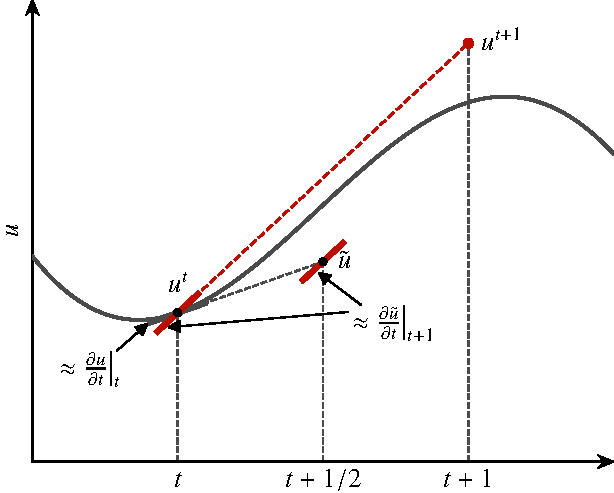
\includegraphics[width=0.6\linewidth]{Pictures/midpoint_method}
	\caption{Midpoint method}
	\label{fig:midpoint_method}
\end{figure}

\subsection{Runge-Kutta Methods}
If we look at Heun's method and the midpoint method, we note that their structure is very similar. We start by computing some intermediate solution, then evaluating the residual of that intermediate solution, and then linearly combining it with the residual of the initial solution. This can be generalized from two stages up to as many stages as we may like, with multiple intermediate solutions being obtained to improve the order of accuracy. Starting from our current solution $u^t$, we will compute $s$ intermediate stage solutions
\begin{equation}
	u_1, u_2, \hdots, u_s,
\end{equation}
where the subscript of $u_i$ denotes the stage number and $s$ is the total number of stages. From these, we can also get the residuals of these intermediate solutions from $R(u_i)$. We compute the intermediate stage solutions from
\begin{equation}
	u_i = u^t + \Delta t \sum_{j=1}^s a_{i,j} R(u_j),
\end{equation}
and the final solution is found from
\begin{equation}
	u^{t+1} = u^t + \Delta t \sum_{i=1}^s b_i R(u_i),
\end{equation}
where $a_{i,j}$ and $b_i$ and a set of constants. These can be compacted into a {\it Butcher Tableau}
\begin{equation}
	\begin{tabular}{c|ccccc}
 
	c   & A \\
 
	\hline
 
	         & b\\
 
	\end{tabular}
    = 	
	\begin{tabular}{c|ccccc}
 
	$c_1$    & $a_{1,1}$ & $\cdots$ & $a_{1,s}$ \\
 
	$\vdots$ & $\vdots$ &  $\ddots$ & $\vdots$\\
 
	$c_s$    & $a_{s,1}$  & $\cdots$ & $a_{s,s}$\\
 
	\hline
 
	         & $b_1$  & $\cdots$ & $b_s$\\
 
	\end{tabular}
\end{equation}
This will yield an explicit scheme if the $A$ matrix is strictly lower-triangular. In that case, we find the solution at any stage is simple a function of the solution of earlier stages. In that case, the method consists of a number of intermediate stage solutions computed using an explicit Euler approach. The following are some example tableaus for commonly-used explicit schemes, including those already introduced.
\begin{figure}[htbp]
	\centering
	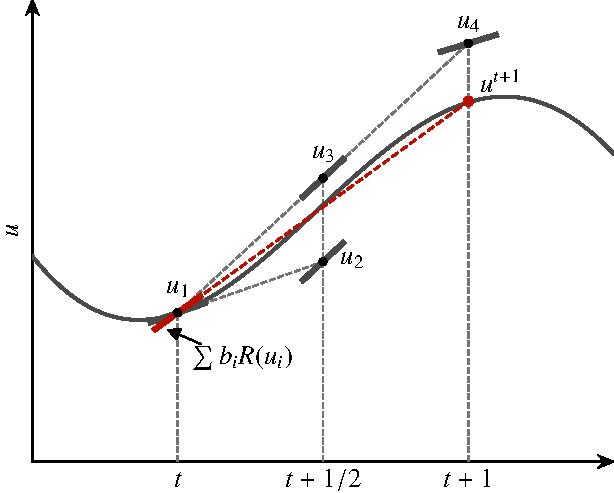
\includegraphics[width=0.6\linewidth]{Pictures/rk_method}
	\caption{Fourth-order four-stage RK method}
	\label{fig:midpoint_method}
\end{figure}

\subsubsection{Explicit Euler}
The explicit Euler method has one stage and is $\mathcal{O}(\Delta t)$ in time.
\begin{equation}
	\begin{tabular}{c|ccccc}
	0   & 0 \\
	\hline
	         & 1\\
	\end{tabular}
\end{equation}

\subsubsection{Heun's Method}
Heun's method has two stages and is $\mathcal{O}(\Delta t^2)$ in time.
\begin{equation}
	\begin{tabular}{c|ccccc}
	0 & \\
	1 & 1 \\
	\hline
	 & $\frac{1}{2}$ & $\frac{1}{2}$\\
	\end{tabular}
\end{equation}

\subsubsection{Explicit Midpoint}
The explicit midpoint method has two stages and is $\mathcal{O}(\Delta t^2)$ in time.
\begin{equation}
	\begin{tabular}{c|ccccc}
	0   & \\
	$\frac{1}{2}$   & $\frac{1}{2}$ \\
	\hline
	         & 0 & 1\\
	\end{tabular}
\end{equation}


\subsubsection{Fourth-Order Runge-Kutta}
The explicit four-stage fourth-order Runge-Kutta method is $\mathcal{O}(\Delta t^4)$ in time.

\begin{equation}
	\begin{tabular}{c|ccccc}
	0   & \\
	$\frac{1}{2}$   & $\frac{1}{2}$ \\
	$\frac{1}{2}$   & 0 & $\frac{1}{2}$ \\
	$1$   & 0 & 0 & 1 \\
	\hline
	         & $\frac{1}{6}$ & $\frac{1}{3}$ & $\frac{1}{3}$ & $\frac{1}{6}$\\
	\end{tabular}
\end{equation}

\section{Implicit}
Going back to the von Neumann analysis section, we note that implicit schemes, those where we evaluated the spatial derivative using the solution at the as-yet-unknown next time step, were unconditionally stable for both linear advection and diffusion. For example, the following scheme was introduced for the linear advection equation
\begin{equation}
	\frac{u_i^{t+1} - u_{i}^t}{\Delta t} +  \alpha \frac{u_i^{t+1} - u_{i-1}^{t+1}}{\Delta x} = 0,
\end{equation}
and the following for the linear diffusion equation
\begin{equation}
  \frac{u_i^{t+1} - u_{i}^t}{\Delta t} - \beta \frac{u_{i-1}^{t+1} - 2u_i^{t+1} + u_{i+1}^{t+1}}{\Delta x^2} = 0.
\end{equation}
These are very similar to our initial schemes, except the spatial operators are evaluated at $t+1$ rather than $t$.

\subsection{Implicit Linear Advection}
We will start our exploration of implicit schemes with the linear advection equation, and rearrange it so all of the terms involving the unknown solution at $t+1$ are of the left-hand side and all of the terms involving the current solution at time $t$ are on the right-hand side
\begin{equation}
	u_i^{t+1} + \sigma \left(u_i^{t+1} - u_{i-1}^{t+1} \right) = u_i^{t},
\end{equation}
where as usual $\sigma = \alpha \Delta t/ \Delta x$. Then, lumping the terms for each grid point on the left-hand side yields
\begin{equation}
	\label{eqn:sh4k18g9}
	(1+\sigma) u_i^{t+1} - \sigma u_{i-1}^{t+1} = u_i^{t}.
\end{equation}
Unlike the explicit schemes, where we could readily rearrange the expression to get $u_i^{t+1}$ alone on the left-hand side, we now have one equation for each grid point that has two unknowns, $u_i^{t+1}$ and $u_{i-1}^{t+1}$, on the left-hand side. This means that in order to get $u_i^{t+1}$ we need to already know $u_{i-1}^{t+1}$, and in order to get $u_{i-1}^{t+1}$ we need to already know $u_{i-2}^{t+1}$, and so on. Hence, it appears we are stuck in a situation where we need to already know the solution at every grid point to get the solution at every other grid point, which we don't yet have.

To get around this, we can recognize that we actually have a large system of linear equations. For each of the $N$ grid points, there is an expression of the form of Equation \ref{eqn:sh4k18g9}, and these involve some linear combination of the $N$ unknown solution values at $t+1$. Hence, we have $N$ equations and $N$ unknowns, yielding a linear system to be solved. This can be written as a linear system of the form
\begin{equation}
	\label{eqn:4h28f95h}
	A \vec{u}^{t+1} = \vec{u}^{t},
\end{equation} 
where, for the case of periodic boundary conditions
\begin{equation}
	A = 
	\begin{bmatrix}
	    1+\sigma & 0 & 0 & \dots  & \sigma \\
	    -\sigma & 1+\sigma & 0 & \dots  & 0 \\
			0 & -\sigma & 1+\sigma & \dots  & 0 \\
	    \vdots & \vdots & \vdots & \ddots & \vdots \\
	    0 & 0 & \dots & -\sigma  & 1+\sigma
	\end{bmatrix},
\end{equation}
is referred to as the Jacobian matrix, and
\begin{equation}
	\vec{u}^{t} = \begin{bmatrix}
	    u_1^t \\
	    u_2^t \\
		u_3^t \\
	    \vdots  \\
	    u_N^t
	\end{bmatrix},
\end{equation}
is a vector of the solution at all grid points at the current time step, and
\begin{equation}
	\vec{u}^{t+1} = \begin{bmatrix}
	    u_1^{t+1} \\
	    u_2^{t+1} \\
		u_3^{t+1} \\
	    \vdots  \\
	    u_N^{t+1}
	\end{bmatrix},
\end{equation}
is a vector of the unknown solution values at the next time step, which is what we are trying to find. Note that the structure of the Jacobian matrix arises directly from writing out the equation for each grid point, and then assembling that as a linear system of equations. It is clear from Equation \ref{eqn:4h28f95h} that we can now solve for all of the solution values in $\vec{u}^{t+1}$ by simply solving a linear system of equations. Hence, we obtain unconditional stability, as discussed in the von Neumann analysis section, at the added cost of having to solve a linear system of equations at each time step. This cost is usually substantial and, hence, implicit schemes are typically used when sufficiently large time steps that are larger than the stability limits of explicit schemes are desired.

\subsection{Implicit Linear Diffusion}
As a second demonstration of an implicit solver, we consider the implicit linear diffusion equation, derived previously as
\begin{equation}
  \frac{u_i^{t+1} - u_{i}^t}{\Delta t} - \beta \frac{u_{i-1}^{t+1} - 2u_i^{t+1} + u_{i+1}^{t+1}}{\Delta x^2} = 0.
\end{equation}
Rearranging this so that all of the known solution values are on the right-hand side and all values at the as yet unknown next time step are on the left-hand side yields
\begin{equation}
  u_i^{t+1} - r (u_{i-1}^{t+1} - 2u_i^{t+1} + u_{i+1}^{t+1}) = u_{i}^t,
\end{equation}
where again $r = \beta \Delta t / \Delta x^2$. Rearranging slight yields
\begin{equation}
  (1+2r)u_i^{t+1} - r (u_{i-1}^{t+1} + u_{i+1}^{t+1}) = u_{i}^t.
\end{equation}
Following the same steps as the linear advection equation, this can be written as a linear system of equations of the form
\begin{equation}
	A \vec{u}^{t+1} = \vec{u}^{t},
\end{equation}
where the Jacobian matrix for periodic boundary conditions can be written as
\begin{equation}
	A = 
	\begin{bmatrix}
	    1+2r & -r & 0 & \dots  & -r \\
	    -r & 1+2r & -r & \dots  & 0 \\
			0 & -r & 1+2r & \dots  & 0 \\
	    \vdots & \vdots & \vdots & \ddots & \vdots \\
	    -r & 0 & \dots & -r & 1+2r
	\end{bmatrix},
\end{equation}
taking note of the locations of the $-r$ terms in the first and last rows that arise from the periodic boundary conditions. Hence, similar to the implicit linear advection scheme, implicit linear diffusion requires the solution of a linear system of equations at each time step. Therefore, it is typically used when the desired time step exceeds the stability limit of available explicit methods. Due to the $\Delta x^2$ scaling of the time step size for diffusion equations, as discussed in the von Neumann analysis section, diffusion operators are often solved using implicit approaches.

\subsection{Implicit Burgers Equation}
In both of the previous sections, we looked at implicit solvers for {\it linear} systems of equations, specifically the linear advection and linear diffusion equations. In this section, we will consider an implicit solver for the {\it non-linear} Burgers equation with a numerical scheme of the form
\begin{equation}
	\frac{u_i^{t+1} - u_{i}^t}{\Delta t} + \frac{1}{2\Delta x}\left( \left(u_i^{t+1} \right)^2 - \left( u_{i-1}^{t+1} \right)^2 \right) =  0.
\end{equation}
Starting from a suitable initial guess for $\vec{u}^{t+1}$, which we will denote as $\vec{u}^{k}$ where $k$ here denotes an iteration number, we can compute the resulting residual at any gridpoint as
\begin{equation}
	r_i = \frac{u_i^{k} - u_{i}^t}{\Delta t} + \frac{1}{2\Delta x}\left( \left(u_i^{k} \right)^2 - \left( u_{i-1}^{k} \right)^2 \right).
\end{equation}
From this we can compute the unsteady residual array $\vec{r}(\vec{u}^{k})$, which determines how well our initial guess satisfies the system of equations. Our objective is to find a value of $\vec{u}^{k}$ such that this residual is zero. Once this is achieved we have found a solution and we can take $\vec{u}^{t+1} = \vec{u}^{k}$.

One of the most powerful approaches to solving this is to use Newton-Raphson. Starting with $\vec{u}^{k}$, our current guess of the solution we will iterate by attempting to enforce that the next iterated values satisfies
\begin{equation}
	\vec{r}(\vec{u}^{k+1}) = 0.
\end{equation}
Via the application of Newton-Raphson we obtain the following expression
\begin{equation}
	\vec{u}^{k+1} = \vec{u}^{k} - \left(\frac{\partial \vec{r}}{\partial \vec{u}^k}\right)^{-1} \vec{r}(\vec{u}^{k}),
\end{equation}
where the Jacobian matrix, for the current Burgers equation discretization, is given by
\begin{equation}
	\frac{\partial \vec{r}}{\partial \vec{u}^k} = 
	\begin{bmatrix}
	    1 + \frac{\Delta t}{\Delta x}u_i^{k} & 0 & 0 & \dots  & - \left(\frac{\Delta t}{\Delta x} u_{i-1}^{k}\right) \\
	    - \left(\frac{\Delta t}{\Delta x} u_{i-1}^{k}\right) & 1 + \frac{\Delta t}{\Delta x}u_i^{k} & 0 & \dots  & 0 \\
			0 & - \left(\frac{\Delta t}{\Delta x} u_{i-1}^{k}\right) & 1 + \frac{\Delta t}{\Delta x}u_i^{k} & \dots  & 0 \\
	    \vdots & \vdots & \vdots & \ddots & \vdots \\
	    0 & 0 & \dots & - \left(\frac{\Delta t}{\Delta x} u_{i-1}^{k}\right)  & 1 + \frac{\Delta t}{\Delta x}u_i^{k}
	\end{bmatrix}.
\end{equation}
Hence, the general procedure for solving nonlinear systems of equations is to start by guessing a solution $\vec{u}^{t+1}$, which is stored as $\vec{u}^{k}$. Typically, a good initial guess is that $\vec{u}^{k} = \vec{u}^{t}$. Using this initial guess, the residual and Jacobian matrices are computed and, via application of Newton-Raphson, an improved guess $\vec{u}^{k+1}$ is obtained. This procedure is then repeated until $\vec{r}(\vec{u}^{k}) \approx 0$, at which point we take $\vec{u}^{t+1} = \vec{u}^{k}$. In the case of linear systems, only one Newton iterations is required. However, for non-linear systems such as Burgers or Navier-Stokes, several Newton iterations are typically required for sufficient convergence.

\chapter{Iterative Methods}
In this implicit time stepping section we reduced each time step to the solution of a linear system of $N$ equations of the form 
\begin{equation}
	A \vec{x} = \vec{b},
\end{equation}
when solving either linear advection or linear diffusion, where $N$ is the number of grid points in the domain. The extra cost of solving this linear system was introduced in order to obtain unconditionally stable schemes, allowing very large time steps to be taken. However, this will only be faster than an explicit approach if the linear system of equations can be solved efficiently. Hence, this section is dedicated to exploring different methods of solving linear systems of equations.

\section{Gaussian Elimination}
Perhaps the most straightforward method for solving a linear system of equations is Guassian elimination. This requires us to invert $A$ and obtain
\begin{equation}
	 \vec{x} = A^{-1} \vec{b}.
\end{equation}
Gaussian elimination is the workhorse of most undergraduate linear algebra courses, and is a straightforward extension of the substitution approach for solving systems of equations taught in highschool. This requires inverting $A$ or an LU decomposition of $A$ and $\vec{b}$ to be formed, and then back substitution to solve for the unknown components of $\vec{x}$.

While Gaussian elimination is well known, its computational cost scales like $\mathcal{O}(N^3)$ where $N$ is the number of unknowns. Hence, as the system of equations, and in our case number of grid points, grows, the computational cost of Gaussian elimination grows cubically. Any undergraduate student should be familiar with trying to solve even $3 \times 3$ linear systems in an exam, let alone $4 \times 4$, or $5 \times 5$. With each additional equation, doing this by hand takes significantly more time. Hence, in the context of CFD, where thousands or millions of equations is common practice, Gaussian elimination is rarely used.

\section{Jacobi Iteration}
Since the formation of $A^{-1}$ is prohibitively expensive for large systems of equations, we will try to find an approximate solution $\vec{x}$, without actually forming $A^{-1}$. This can be done iteratively, and the first approach we will introduce is Jacobi iteration. In Jacobi iteration, we start by splitting $A$ into $L$, $D$, and $U$, and are its strictly lower-triangular, diagonal, and strictly upper-triangular components. This allows us to write our linear system as
\begin{equation}
	(L+D+U) \vec{x} = \vec{b},
\end{equation}
where
\begin{equation}
	A = 
	\begin{bmatrix}
	    a_{11} & a_{12} & a_{13} & \dots  & a_{1n} \\
	    a_{21} & a_{22} & a_{23} & \dots  & a_{2n} \\
			a_{31} & a_{32} & a_{33} & \dots  & a_{3n} \\
	    \vdots & \vdots & \vdots & \ddots & \vdots \\
	    a_{n1} & a_{n2} & a_{n3} & \dots  & a_{nn}
	\end{bmatrix},
\end{equation}
\begin{equation}
	L = 
	\begin{bmatrix}
	    0 & 0 & 0 & \dots  & 0 \\
	    a_{21} & 0 & 0 & \dots  & 0 \\
			a_{31} & a_{32} & 0 & \dots  & 0 \\
	    \vdots & \vdots & \vdots & \ddots & \vdots \\
	    a_{n1} & a_{n2} & a_{n3} & \dots  & 0
	\end{bmatrix},
\end{equation}
\begin{equation}
	D = 
	\begin{bmatrix}
	    a_{11} & 0 & 0 & \dots  & 0 \\
	    0 & a_{22} & 0 & \dots  & 0 \\
			0 & 0 & a_{33} & \dots  & 0 \\
	    \vdots & \vdots & \vdots & \ddots & \vdots \\
	    0 & 0 & 0 & \dots  & a_{nn}
	\end{bmatrix},
\end{equation}
\begin{equation}
	U = 
	\begin{bmatrix}
	    0 & a_{12} & a_{13} & \dots  & a_{1n} \\
	    0 & 0 & a_{23} & \dots  & a_{2n} \\
			0 & 0 & 0 & \dots  & a_{3n} \\
	    \vdots & \vdots & \vdots & \ddots & \vdots \\
	    0 & 0 & 0 & \dots  & 0
	\end{bmatrix}.
\end{equation}
Now if $\vec{x}$ is a solution to the linear system then the following is valid
\begin{equation}
	L\vec{x} + D\vec{x} + U\vec{x} = \vec{b}.
\end{equation}
We can now rearrange this expression
\begin{equation}
	D\vec{x} = \vec{b} - (L+U)\vec{x},
\end{equation}
and by inverting $D$ we get
\begin{equation}
	\vec{x} = D^{-1}\left[ \vec{b} - (L+U)\vec{x} \right].
	\label{eqn:f928bs7g}
\end{equation}
At this point, it is important to know that while inverting $A$ is very expensive, inverting just its diagonal values in $D$ is trivial.

We note that if $\vec{x}$ is a solution to the linear system of equations, then Equation \ref{eqn:f928bs7g} will be satisfied exactly, but if we already had the exact solution there would be no point in this exercise. However, if we look again at Equation \ref{eqn:f928bs7g} it has an interesting form. We note that if we insert some guess for $\vec{x}$ into the right-hand side, we get out a modified $\vec{x}$ on the left-hand side. This allows us to define Jacobi iteration as
\begin{eqBox}
\begin{equation}
	\vec{x}_{n+1} = D^{-1}\left[ \vec{b} - (L+U)\vec{x}_n \right],
	\label{eqn:3jc810fg}
\end{equation}
\end{eqBox}
where $\vec{x}_n$ is an approximate solution, and $\vec{x}_{n+1}$ is an updated approximation. Then we can simply pass $\vec{x}_{n+1}$ back through this formulation to obtain $\vec{x}_{n+2}$, and so on, iterating to a final solution when the value of $\vec{x}$ converges. This can also be written in an element-by-element manner as
\begin{eqBox}
\begin{equation}
	x_i^{n+1} = \frac{1}{a_{i,i}}\left(b_i - \sum_{i \neq i} a_{i,j}x_j^k \right), \: \: i = 1,2,\hdots,n.
\end{equation}
\end{eqBox}
Each step of Jacobi iteration requires $\mathcal{O}(N^2)$ operations, hence, we can expect Jacobi to outperform Gaussian elimination, as long as we need fewer iterations than there are rows in the system of equations. Furthermore, in CFD it is usually sufficient to converge $\vec{x}$ to some finite level of precision.

To demonstrate the utility of Jacobi iteration we will use a simple example of a $3 \times 3$ system of equations. Starting with 
\begin{equation}
	A = 
	\begin{bmatrix}
	    10 & 2 & 4 \\
	    6 & 8 & 4 \\
			2 & 3 & 9
	\end{bmatrix},
\end{equation}
and
\begin{equation}
	\vec{b} = \begin{bmatrix}
	    1 \\
	    2 \\
			3
	\end{bmatrix},
\end{equation}
we obtain the following for $L$, $D$, and $U$
\begin{equation}
	L = 
	\begin{bmatrix}
	    0 & 0 & 0 \\
	    6 & 0 & 0 \\
			2 & 3 & 0
	\end{bmatrix},
\end{equation}
\begin{equation}
	D = 
	\begin{bmatrix}
	    10 & 0 & 0 \\
	    0 & 8 & 0 \\
			0 & 0 & 9
	\end{bmatrix},
\end{equation}
\begin{equation}
	U = 
	\begin{bmatrix}
	    0 & 2 & 4 \\
	    0 & 0 & 4 \\
			0 & 0 & 0
	\end{bmatrix}.
\end{equation}
Furthermore, we can easily invert $D$ to get
\begin{equation}
	D^{-1} = 
	\begin{bmatrix}
	    \frac{1}{10} & 0 & 0 \\
	    0 & \frac{1}{8} & 0 \\
			0 & 0 & \frac{1}{9}
	\end{bmatrix}.
\end{equation}
Now we can start with some initial guess, lets say
\begin{equation}
	\vec{x_0} = \begin{bmatrix}
	    0 \\
	    0 \\
			0
	\end{bmatrix}.
\end{equation}
Convergence can usually be accelerated by using a good initial guess, for example, that the solution at the next time step in our CFD simulation is the same as the current solution.

Now with our initial Guess and all terms from the right-hand side of Equation \ref{eqn:3jc810fg} defined, we can compute
\begin{equation}
	\vec{x}_{1} = D^{-1}\left[ \vec{b} - (L+U)\vec{x}_0 \right] = \begin{bmatrix}
	    0.1000 \\
	    0.2500 \\
			0.3333
	\end{bmatrix}.
\end{equation}
Repeating this iteration a few times yields
\begin{equation}
	\vec{x}_{2} = D^{-1}\left[ \vec{b} - (L+U)\vec{x}_1 \right] = \begin{bmatrix}
	    -0.0833 \\
	    0.0083 \\
			0.2277
	\end{bmatrix},
\end{equation}
\begin{equation}
	\vec{x}_{3} = D^{-1}\left[ \vec{b} - (L+U)\vec{x}_2 \right] = \begin{bmatrix}
	    0.0072 \\
	    0.1986 \\
			0.3490
	\end{bmatrix},
\end{equation}
and after 15 iterations we obtain
\begin{equation}
	\vec{x}_{15} = D^{-1}\left[ \vec{b} - (L+U)\vec{x}_14 \right] = \begin{bmatrix}
	    -0.0465 \\
	    0.1356 \\
			0.2984
	\end{bmatrix},
\end{equation}
which is very close to the exact solution
\begin{equation}
	\vec{x} = \begin{bmatrix}
	    -0.0465 \\
	    0.1357 \\
			0.2984
	\end{bmatrix}.
\end{equation}
Hence, after only 15 iterations Jacobi was able to converge to approximately four digits, without having to ever directly invert the $A$ matrix.
\begin{jupyternote}
	Check out the Iterative Methods Jupyter notebook \href{\binderurl}{\underline{here}}. You can also download the files from the Gitlab repository \href{\repourl}{\underline{here}}.
\end{jupyternote}
\section{Gauss Seidel Iteration}
With the idea of Jacobi iteration outlined above, we may wonder whether similar more efficient approaches exist. The first of these, with a very similar derivation to Jacobi, is the Gauss-Seidel method. Starting from our split $A$ matrix in the Jacobi section
\begin{equation}
	(L+D+U) \vec{x} = \vec{b},
\end{equation}
we rearrange it as
\begin{equation}
	(L + D)\vec{x} = \vec{b} - U\vec{x}.
\end{equation}
If we consider the $(L+D)$ matrix we note that it is lower-triangular. While not as trivial to invert as $D$ in Jacobi iteration, inverting $(L+D)$ can be done quickly via back-substitution. Hence, we can write
\begin{equation}
	\vec{x} = (L + D)^{-1}\left[ \vec{b} - U\vec{x} \right].
\end{equation}
Similar to Jacobi, we notice that if we insert an estimate for $\vec{x}$ on the right-hand side, we obtain an updated estimate on the left-hand side. Hence, we define Gauss-Seidel iteration as
\begin{eqBox}
\begin{equation}
	\vec{x}_{n+1} = (L + D)^{-1}\left[ \vec{b} - U\vec{x}_n \right].
\end{equation}
\end{eqBox}
Also, similar to Jacobi this can be performed in a element-wise manner for each component of the solution via
\begin{eqBox}
\begin{equation}
	x_i^{n+1} = \frac{1}{a_{i,i}}\left(b_i - \sum_{j=1}^{i-1} a_{i,j}x_j^{n+1} - \sum_{j=i+1} a_{i,j}x_j^n \right), \: \: i = 1,2,\hdots,n.
\end{equation}
\end{eqBox}
It is clear from this that Gauss-Seidel amounts to simply a Jacobi iteration but using the most up to date entries $a_{i,j}x_j^n$ or $a_{i,j}x_j^{n+1}$ as they are available. Usually, the additional cost of computing $(L + D)^{-1}$, relative to simply computing $D^{-1}$ with Jacobi, significantly reduces the number of iterations and total computational cost.

Going back to our example from Jacobi iteration, we have
Now with our initial Guess and all terms from the right-hand side of Equation \ref{eqn:3jc810fg} defined, we can compute
\begin{equation}
	\vec{x}_{1} = (L + D)^{-1}\left[ \vec{b} - U\vec{x}_0 \right] = \begin{bmatrix}
	    0.1000 \\
	    0.1750 \\
			0.2527
	\end{bmatrix}.
\end{equation}
Repeating this iteration a few times yields
\begin{equation}
	\vec{x}_{2} = (L + D)^{-1}\left[ \vec{b} - U\vec{x}_1 \right] = \begin{bmatrix}
	    -0.0361 \\
	    0.1506 \\
			0.2911
	\end{bmatrix},
\end{equation}
\begin{equation}
	\vec{x}_{3} = (L + D)^{-1}\left[ \vec{b} - U\vec{x}_2 \right] = \begin{bmatrix}
	    -0.0465 \\
	    -0.0467 \\
			0.2982
	\end{bmatrix},
\end{equation}
and after only 5 iterations we obtain
\begin{equation}
		\vec{x}_{5} = (L + D)^{-1}\left[ \vec{b} - U\vec{x}_4 \right] = \begin{bmatrix}
	    -0.0465 \\
	    0.1358 \\
			0.2984
	\end{bmatrix},
\end{equation}
which is very close to the exact solution
\begin{equation}
	\vec{x} = \begin{bmatrix}
	    -0.0465 \\
	    0.1357 \\
			0.2984
	\end{bmatrix}.
\end{equation}
Hence, after only 5 iterations, or three times as fast as Jacobi in this case, Gauss Seidel was able to converge to approximately four digits.
\begin{jupyternote}
	Check out the Iterative Methods Jupyter notebook \href{\binderurl}{\underline{here}}. You can also download the files from the Gitlab repository \href{\repourl}{\underline{here}}.
\end{jupyternote}
\section{Successive Over-Relaxation}
When using the Gauss-Seidel approach, we often observe that the iterated solutions converge gradually to the exact solution for $\vec{x}$. That is, each iteration takes a step towards the exact solution in a somewhat uniform manner. We can exploit this by simply extrapolating each iteration to move a bit further towards the exact solution, which is known as Successive Over-Relaxation (SOR). This is usually done to accelerate convergence, but as will be discussed later, it can be used to also stabilize convergence.
\begin{figure}[htbp]
	\centering
	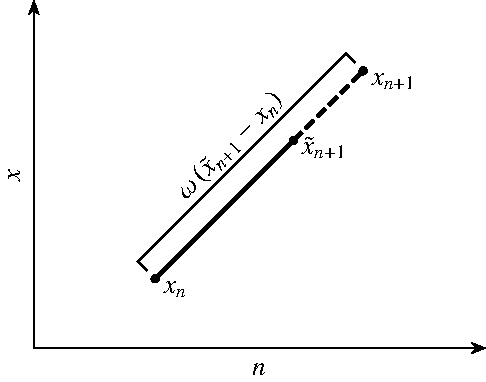
\includegraphics[width=0.5\linewidth]{Pictures/itermethods_sor}
	\caption{Successive Over-Relaxation method.}
	\label{fig:sor}
\end{figure}

With SOR we simply apply a Gauss Seidel iteration to our current approximation of the solution, $\vec{x}_n$. We store the results of this Gauss-Seidel iteration temporarily as $\tilde{\vec{x}}_{n+1}$. Then, using the SOR approach, we linearly project our updated solution using our current and previous approximations, as shown in Figure~\ref{fig:sor}. Hence,
\begin{eqBox}
\begin{equation}
	\vec{x}_{n+1} = \omega \tilde{\vec{x}}_{n+1} + (1-\omega) \vec{x}_n.
\end{equation}
\end{eqBox}
where $\omega$ is referred to as therelaxation factor. We note that when $\omega=1$ we recover the original Gauss Seidel approach. When $\omega>1$ we say it is over-relaxed, usually accelerating convergence but also potentially causing the iterations to diverge. When $\omega<1$ we say it is under-relaxed, which usually improves stability, but reduces the rate of convergence. In general, a suitable value for the relaxation factor is within the range
\begin{equation}
	0 \leq \omega \leq 2,
\end{equation}
and values of $\omega > 2$ will diverge. Typically, $\omega$ is chosen to be as large as possible, without causing the iterations to diverge.

\section{Assessing Convergence}
In typical CFD applications, the user provides a desired convergence tolerance for solving the linear system of equations. To assess this, we introduce the concept of a residual. In the case of an exact solution to a linear system, we would expect
\begin{equation}
	A \vec{x} - \vec{b} = 0.
\end{equation}
However, since our solution at any given iteration is only an approximate solution then
\begin{equation}
	A \vec{x}_n - \vec{b} = \vec{r},
\end{equation}
where $\vec{r}$ is referred to as the residual and measures how well our current approximate solution satisfies the system of equations being solved. While $\vec{r}$ gives detailed information about how well each equation in the entire system is being solved, it is typically more useful to provide the user with a norm, such as $\| \vec{r} \|_2$ or $\| \vec{r} \|_\infty$, giving a single measure of convergence. Then, iterations are continued until this residual norm converges to within the desired tolerance. It is also important to note that if the convergence tolerance is too high, it can result in a loss of accuracy or stability in the CFD simulation. Hence, particular care must be chosen in how to select the desired convergence tolerance.

\section{Multigrid}
It is important to note that both Jacobi and Gauss-Seidel iterations require $\mathcal{O}(N^2)$ operations per iteration, they will typically be much faster than Gaussian elimination, provided the number of iterations is relatively small. However, the computational cost will still increase rapidly with the number of grid points. Ideally, we would like an iterative method that will converge with $\mathcal{O}(N)$ operations, resulting in a computational cost that varies linearly with the number of grid points.

An important observation regarding the aforementioned iterative methods, such as Jacobi and Gauss-Seidel, is that they tend to converge {\it high-wavenumber} features, those that span only a few grid points, very quickly. In contrast, {\it low-wavenumber} features, those that span a large number of grid points, converge relatively slowly. The general idea behind the multigrid method is to use an additional coarse grid to converge these large scale structures. Since this additional grid is coarse, it is relatively cheap per iteration, since it contains significantly fewer grid points and unknowns. Also, the low-wavenumber features on the fine grid appear as higher-wavenumber features on the coarse grid and, hence, they converge quickly there. This procedure can then be extended to a large number of grid levels, resulting in the {\it multigrid} method.

As an example, we will describe a two-level multigrid method for solving the linear system of equations
\begin{equation}
	A_h \vec{x}_h = \vec{b}_h,
\end{equation}
where the subscript $h$ denotes that this is the initial system of equations the on fine grid, denoted by $\Omega_h$. Ultimately, we want to obtain the final solution to this linear system, $\vec{x}_h$, with as little computational cost as possible. From here, we will recall that the residual on the fine grid can be defined as
\begin{equation}
	\vec{r}_h = \vec{b}_h - A_h \vec{x}_{h,n},
\end{equation}
where $\vec{x}_{h,n}$ is our current iterated estimate of the true solution. We will also define the error on the fine grid as simply the difference between the exact solution and the current iterated solution
\begin{equation}
	\vec{e}_{h,n} = \vec{x}_{h} - \vec{x}_{h,n}.
\end{equation}
Rearranging this expression for the error yields
\begin{equation}
	\vec{x}_{h,n} =  \vec{x}_{h} - \vec{e}_{h,n}.
\end{equation}
Substituting this into our expression for the expression for the residual yields
\begin{equation}
	\vec{r}_h = \vec{b}_h - A_h (\vec{x}_{h} - \vec{e}_{h,n}),
\end{equation}
and finally
\begin{equation}
	A_h \vec{e}_{h,n} = \vec{r}_h.
\end{equation}
Hence, similar to the solution, the error between the exact and current iterated solution also obeys a linear system of equations. In the multigrid method, it is this error on the fine grid that gets projected to the coarse grid, and that is what is solved. The general multigrid process is as follows:
\begin{itemize}
	\item {\it Relax} $A_h \vec{x}_h = \vec{b}_h$ using $n$ iterations of Jacobi or Gauss-Seidel to obtain $\vec{x}_{h,n}$
	\item {\it Compute} the residual on the fine grid level using $\vec{r}_h = \vec{b}_h - A_h \vec{x}_{h,n}$
	\item {\it Restrict} the residual from $\Omega_h \rightarrow \Omega_{2h}$ using $\vec{r}_{2h} = I_{h}^{2h} \vec{r}_h$
	\item {\it Solve} $A_{2h} \vec{e}_{2h,n} = \vec{r}_{2h}$ using Jacobi, Gauss-Seidel, or Gaussian elimination
	\item {\it Prolongate} the error from $\Omega_{2h} \rightarrow \Omega_{h}$ using $\vec{e}_{h} = I_{2h}^{h} \vec{e}_{2h}$
	\item {\it Correct} the solution on the fine grid using $\vec{x}_{h,n} = \vec{x}_{h,n} + \vec{e}_{h}$
	\item {\it Repeat} from the first step until the system of equations on the fine grid converges
\end{itemize}
In the above approach, we have introduced two new operators, specifically the restriction operator $I_{h}^{2h}$ and the prolongation operator $I_{2h}^{h}$ that are responsible for transferring data from the fine to coarse grid, and vice-versa. If we look at their required shapes, we find that $I_{h}^{2h} \in N_{2h} \times N_h$, where $N_{2h}$ is the number of degrees of freedom on the coarse grid and $N_h$ is the number of degrees of freedom on the fine grid. In contrast, the prolongation operator is of dimension $I_{2h}^{h} \in N_{h} \times N_{2h}$. Consider the one-dimensional example case shown in Figure \ref{}, where $\Omega_{2h}$ is coarser than $\Omega_h$ in the sense that every other grid point is omitted. One simple option is to simply {\it linearly} interpolate the error from the coarse grid to the fine grid. This would give the following prolongation operator matrix
\begin{equation}
	I_{2h}^{h} = 
	\begin{bmatrix}
	    1 & 0 & 0 & 0 \\
			\frac{1}{2} & \frac{1}{2} & 0 & 0 \\
			0 & 1 & 0 & 0 \\
			0 & \frac{1}{2} & \frac{1}{2} & 0 \\
	    0 & 0 & 1 & 0 \\
			0 & 0 & \frac{1}{2} & \frac{1}{2} \\
			0 & 0 & 0 & 1 \\
			\frac{1}{2} & 0 & 0 & \frac{1}{2}
	\end{bmatrix},
\end{equation}
assuming periodic boundary conditions and a linear interpolation between the intermediate points. Now, to get the restriction operator, which transfers data from the fine grid to the coarse grid, we use
\begin{equation}
	I_{h}^{2h} = c (I_{2h}^{h})^T,
\end{equation}
where $c$ is a constant chosen such that all row sums of $I_{h}^{2h}$ are unity. This expands to
\begin{equation}
	I_{h}^{2h} = c
	\begin{bmatrix}
	    1 & \frac{1}{2} & 0 & 0 & 0 & 0 & 0 & \frac{1}{2} \\
			0 & \frac{1}{2} & 1 & \frac{1}{2} & 0 & 0 & 0 & 0 \\
			0 & 0 & 0 & \frac{1}{2} & 1 & \frac{1}{2} & 0 & 0 \\
			0 & 0 & 0 & 0 & 0 & \frac{1}{2} & 1 & \frac{1}{2} \\
	\end{bmatrix},
\end{equation}
and taking $c = 1/2$ yields
\begin{equation}
	I_{h}^{2h} =
	\begin{bmatrix}
	    \frac{1}{2} & \frac{1}{4} & 0 & 0 & 0 & 0 & 0 & \frac{1}{4} \\
			0 & \frac{1}{4} & \frac{1}{2} & \frac{1}{4} & 0 & 0 & 0 & 0 \\
			0 & 0 & 0 & \frac{1}{4} & \frac{1}{2} & \frac{1}{4} & 0 & 0 \\
			0 & 0 & 0 & 0 & 0 & \frac{1}{4} & \frac{1}{2} & \frac{1}{4} \\
	\end{bmatrix},
\end{equation}
satisfying the condition of having row sums of unity. Now that we have the restriction and prolongation operators, the last step is to find the linear system of equations on the coarse grid. This is found via
\begin{equation}
	A_{2h} = I_{h}^{2h} A_h I_{2h}^{h}.
\end{equation}
Hence, starting from the linear system of equations and the node locations on the coarse and fine grids, the first step for constructing the system on the coarse grid level is to provide a suitable prolongation operator to take data from this coarse to the fine grid. From this, one obtains the corresponding restriction operator, and finally the operator matrix on the coarse grid. Now, all of the required data is available to complete the multigrid procedure. We note that the above procedure describes a two-level multigrid method. However, this can be readily extended to any number of multigrid stages, and the smallest grid levels are typically coarse enough to be solved directly using Gaussian elimination. Furthermore, these grid levels can be traversed in different orders. For example, the V-cycle, W-cycle, and Full Multigrid cycle shown in Figure \ref{fig:multigrid}. Typically, each cycle spends the majority of its iterations on the coarsest grid levels, since iterations are relatively inexpensive here. Iterations are only performed on the finest grid level sparingly, and to converge the highest-wavenumber features in the flow.
\begin{figure}[htbp]
	\centering
	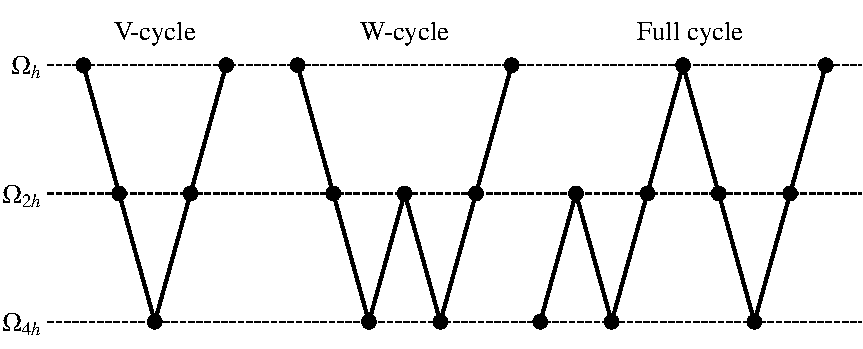
\includegraphics[width=0.8\linewidth]{Pictures/multigrid}
	\caption{Common multigrid methods using three refinement levels}
	\label{fig:multigrid}
\end{figure}

\chapter{Applications}
\section{An Euler Solver}
In this section, we will describe how to develop a two-dimensional solver for the Euler equations on a periodic domain. This will be approximated using finite difference methods in space and advanced in time using an explicit Runge-Kutta method. 

Note that the Euler equations in two dimensions can be expanded as
\begin{equation}
	\label{eqn:5js81pgl}
	\frac{\partial \vec{w}}{\partial t} + \frac{\partial{\vec{F}}}{\partial x} + \frac{\partial{\vec{G}}}{\partial y} = 0,
\end{equation}
where
\begin{equation}
	\label{eqn:dh691kgu}
	\vec{w} = [\rho,\rho u, \rho v, \rho E]^T,
\end{equation}
is a vector of the conserved variables, $u$ and $v$ are the velocity components, and $E$ is the specific energy. The fluxes can be found directly as a function of the solution
\begin{equation}
	\label{eqn:sm5j29dj}
	\vec{F} = [\rho u,\rho u^2 + p, \rho uv, u(\rho E+p)]^T,
\end{equation}
and
\begin{equation}
	\label{eqn:029as5ns}
	\vec{G} = [\rho v,\rho u v, \rho v^2+p, v(\rho E+p)]^T,
\end{equation}
where
\begin{equation} 
	p = \rho R T,
\end{equation}
is the ideal gas law where $R$ is the gas constant and $T$ is temperature. Through some manipulation of the ideal gas law it can be shown that this can be written in an alternative form
\begin{equation} 
	p = (\gamma -1) \rho \left(E - \frac{1}{2}\left(u^2 + v^2 \right) \right),
\end{equation}
that no longer requires the gas constant, and where $\gamma$ is the ratio of specific heats. Hence, given the value of the solution at any point in the domain, and the ideal gas law, we can determine both of the flux components.

It is worth taking a moment to consider this set of equations. Using the finite difference approach, we will store the conserved variables, specifically mass, momentum, and energy, at each grid point. From Equation \ref{eqn:5js81pgl}, it is then possible to then get the time derivative of the solution at all of these grid points, provided we can compute the fluxes and their derivatives in space. This simply requires the specification of suitable finite difference methods for approximating the derivatives in space.

Now consider a two-dimensional domain of length $L_x$ and $L_y$ in each direction that is discretized using a grid of $N_x$ and $N_y$ equidistant points. Using periodic boundary conditions, the grid spacing between adjacent points is
\begin{equation}
	\Delta x = \frac{L_x}{N_x},
\end{equation}
in the x-direction and
\begin{equation}
	\Delta y = \frac{L_y}{N_y},
\end{equation}
in the y-direction. The current value of the solution is stored at all grid points and denoted by $\vec{w}_{i,j}^t$ where $i$ and $j$ are the grid point indices and $t$ is the time level. We also store the coordinates of each grid point as $\vec{x}_{i,j}$, where 
\begin{equation}
	\vec{x}_{i,j} = [x_{i,j},y_{i,j}]^T.
\end{equation}
Provided an initial condition, the value of the solution is known at each grid point at the start of the simulation. Then the fluxes at each grid point can be calculated according to Equation \ref{eqn:sm5j29dj} and Equation \ref{eqn:029as5ns}. Hence, at every grid point we will now have $\vec{w}_{i,j}^t$, $\vec{F}_{i,j}^t$, and $\vec{G}_{i,j}^t$. Now using, for example, second-order central differences in space, we can write
\begin{equation}
	\frac{d \vec{w}_{i,j}^t}{d t} + \frac{\vec{F}_{i+1,j}^t-\vec{F}_{i-1,j}^t}{2\Delta x} + \frac{\vec{G}_{i,j+1}^t-\vec{G}_{i,j-1}^t}{2\Delta y} + \mathcal{O}(\Delta x^2,\Delta y^2) = 0.
\end{equation}
Hence, given a value of the solution at every grid point, the fluxes, their divergence, and finally the time rate of change of the solution at each grid point can be determined. Then, using an appropriate temporal scheme, such as the classical RK$_{4,4}$ method, this system of equations can be advanced to the next time step.

As an example, we will consider advection of an isentropic vortex having the initial condition
\begin{eqnarray}
\begin{split}
\rho & = \left[1-\frac{S^2Ma^2(\gamma-1)e^{2f}}{8\pi^2}\right]^{\frac{1}{\gamma-1}},\\
u& = \frac{S(y-y_c)e^f}{2\pi R},\\
v& = 1-\frac{S(x-x_c)e^f}{2\pi R},\\
p& = \frac{\rho^\gamma}{\gamma Ma^2},
\end{split}
\end{eqnarray}
where $f = (1-(x-x_c)^2-(y-y_c)^2)/2R^2$, $S = 13.5$ is the strength of the vortex, $R=1.5$ is the characteristic vortex radius, $\gamma = 1.4$, the Mach number is $Ma = 0.4$, and $x_c$ and $y_c$ are the initial location of the vortex center. This initial condition is isentropic and, hence, without any viscous effects, the exact solution consists of the vortex maintaining its initial shape and simply advecting with the mean flow at a vertical velocity of unity. Since the domain is periodic, the vortex will eventually return to its initial condition, and at this point, we can evaluate an error norm of the density field of the form
\begin{equation}
	\| \rho \|_2 = \sqrt{\frac{\sum_{i=1}^{N_x} \sum_{j=1}^{N_y} \left(\rho_{i,j} - \rho_{e,i,j}\right)^2}{N_x N_y}},
\end{equation}
where $\rho_{e,i,j}$ is the exact solution at a grid point, which is equal to the initial condition at time $t = L_y/1$ since the vertical velocity is unity.

\section{A Navier-Stokes Solver}
\begin{figure}[htbp]
	\centering
	\includegraphics[width=0.6\linewidth]{Pictures/cavity_flow}
	\caption{Lid-driven cavity flow problem}
	\label{fig:lidcavity}
\end{figure}
In order to solve the Navier-Stokes equations, we can readily extend the two-dimensional Euler solver outlined in the previous section. Here we will demonstrate how to solve the Navier-Stokes equations for a classical lid-driven cavity flow problem, as shown in Figure \ref{fig:lidcavity}. Again, this will be discretized using the finite difference method in space, with grid spacings
\begin{equation}
	\Delta x = \frac{L_x}{(N_x-1)},
\end{equation}
and
\begin{equation}
	\Delta y = \frac{L_y}{(N_y-1)},
\end{equation}
to ensure that grid points are included along all edges of the domain.

Starting with the Navier-Stokes equations in two dimensions, we note that they can also be expanded in the following form
\begin{equation}
	\label{eqn:5js81pgl}
	\frac{\partial \vec{w}}{\partial t} + \frac{\partial{\vec{F}}}{\partial x} + \frac{\partial{\vec{G}}}{\partial y} = 0,
\end{equation}
where again
\begin{equation}
	\vec{w} = [\rho,\rho u, \rho v, \rho E]^T,
\end{equation}
is a vector of the conserved variables. In addition, unlike the isentropic vortex test case, the lid-driven cavity flow problem requires boundary conditions to be applied at the edges of the domain. In this case, we need to enforce the no-slip boundary conditions on all four walls. In addition, we will enforce that the walls are isothermal. This is achieved by setting
\begin{equation}
	u_b = u_w, \: \:
	v_b = v_w,
\end{equation}
where $u_w = v_w = 0$ on all boundaries, except for the top plate where $u_w$ is specified to be consistent with the chosen Reynolds number. Then, the temperature at the boundary is fixed at
\begin{equation}
	T_b = T_w,
\end{equation}
which is specified to be the same temperature as the initial gas in the domain. In order to get the density at the wall, the pressure is first projected from the interior onto the boundary, and 
\begin{equation}
	p_b = p_+,
\end{equation}
where $p_+$ is the pressure at the first grid point off of the wall. Finally, the density can be obtained from the ideal gas law with the specified wall temperature and the pressure, and the state vector at the wall $\vec{w}_b$ can be constructed.

For the Navier-Stokes equations, the flux functions can now be written as the sum of their respective inviscid and viscous components, such that $\vec{F} = \vec{F}_i + \vec{F}_v$ and $\vec{G} = \vec{G}_i + \vec{G}_v$, and $\vec{F}_i$ and $\vec{G}_i$ are the inviscid flux, which are still
\begin{equation}
	\vec{F}_i = [\rho u,\rho u^2 + p, \rho uv, u(\rho E+p)]^T,
\end{equation}
and
\begin{equation}
	\vec{G}_i = [\rho v,\rho u v, \rho v^2+p, v(\rho E+p)]^T.
\end{equation}
Furthermore, the viscous fluxes $\vec{F}_v$ and $\vec{G}_v$ are expanded to
\begin{equation}
	\vec{F}_v = [0,-\tau_{xx}, -\tau_{xy}, q_x-u\tau_{xx}-v\tau_{xy}]^T,
\end{equation}
and
\begin{equation}
	\vec{G}_v = [0,-\tau_{xy}, -\tau_{yy}, q_y-u\tau_{xy}-v\tau_{yy}]^T,
\end{equation}
where 
\begin{equation}
	q_x = -k \frac{\partial T}{\partial x},
\end{equation} 
\begin{equation}
 q_y = -k \frac{\partial T}{\partial y},
\end{equation} 
are the heat fluxes, $k$ is the thermal conductivity and
\begin{equation}
	\tau_{xx} = \frac{2}{3}\mu\left(2 \frac{\partial u}{\partial x} - \frac{\partial v}{\partial y} \right),
\end{equation}
\begin{equation}
	\tau_{yy} = \frac{2}{3}\mu\left(2 \frac{\partial v}{\partial y} - \frac{\partial y}{\partial x} \right),
\end{equation}
\begin{equation}
	\tau_{xy} = \mu \left(\frac{\partial u}{\partial y} + \frac{\partial v}{\partial x}\right).
\end{equation}
We note that, unlike the Euler equations, we cannot obtain the viscous fluxes directly from the solution, since they also require the gradients of the velocity components and temperature. To obtain these gradients, we will simply use central differences in the middle of the domain. For example, for the gradient of $u$ the following finite difference methods can be used
\begin{equation}
	\frac{\partial u}{\partial x} = \frac{u_{i+1,j}^t - u_{i-1,j}^t}{2 \Delta x},
\end{equation}
\begin{equation}
	\frac{\partial u}{\partial y} = \frac{u_{i,j+1}^t - u_{i,j-1}^t}{2 \Delta y}.
\end{equation}
However, these finite difference methods will not work for computing the velocity and temperature gradients of the solution at the boundaries of the domain, since they would require points outside of the computational domain. Instead, one-sided stencils can be used at the wall. For example, the following stencil can be used on the left-hand side boundary of the domain
\begin{equation}
	\frac{\partial u}{\partial x} = \frac{-u_{i,3} + 4u_{i,2} - 3u_{i,1}}{2\Delta x},
\end{equation}
and along the length of each wall, we will take the derivative to be zero. For example, on the left and right-hand side boundaries this will yield
\begin{equation}
	\frac{\partial u}{\partial y} = 0.
\end{equation}

Using these stencils we now have the solution vector at each grid point in the domain, and derivatives of the velocity and temperature field at each point in the domain. Now, at every point the inviscid and viscous fluxes can be computed. With these obtained, the same finite difference stencils can be applied to get the divergence of these fluxes, completing the right hand side of the conservation law. Finally, the solution and be advanced in time using a suitable explicit Runge-Kutta method for the temporal term.